\chapter{Análise Bibliográfica sobre Análise de Dados integradas em Nuvem para auxílio de Fenômenos Sociais, por Guilherme Oliveira Loiola\label{chap:bibliometria:guioliunb}}

\section{Planejamento do estudo\label{MASSA:coleta}}
O planejamento o  desenho do estudo deve descrever as motivações, questões de interesse, escopo, limitações e objetivos do trabalho.

O planejamento do estudo deve motivar o tema escolhido e o interesse do autor.

No caso do meu trabalho, as perguntas que o nortearam foram:
\begin{itemize}
    \item Qual a base de conhecimentos científicos produzida com análises de dados com auxílio da computação em nuvem voltada à compreensão de fenômenos sociais? 
    \item Como a capacidade de processamento da nuvem está proporcionando análises sociais mais precisas e eficientes? 
    \item Quais são as principais aplicações de interesse da comunidade científica diante da evolução tecnológica dos últimos anos?
    \item Quais os principais métodos de análise e ferramentas de aplicação nos problemas atuais?
\end{itemize}

\subsection{O que já existe de pesquisa bibliométrica sobre esse tema?}

\cite{ma_method_2020} realizou uma pesquisa que visava  combinar a capacidade de processamento da computação em nuvem com os algoritmos de inteligência artificial para auxiliar na identificação de padrões e criação de metodologias de tratamento para dificuldades enfrentadas na psiquiatria.

Assim como \cite{archenaa_interactive_2016} que promoveu um estudo enfrentando desafios da saúde utilizando computação em nuvem.


\subsection{Uso do Bibliometrix e Biblioshiny}
Serão usadas a ferramenta e o \textit{workflow} proposto pelos autores do pacote Bibliometrix.

\subsection{Limitações} O exercício relatado foi feito em uma semana, envolvendo de um autor. As bases de dados foram buscadas na plataforma WoS,


\section{Coleta de dados\label{MASSA:coleta}}

A coleta de dados feita usando o WoS no dia 08 de janeiro de 2022, acessado por meio do Portal de Periódicos da CAPES.

Foram feitas buscas na coleções \textbf{Web of Science - Coleção Principal (Clarivate Analytics) } que possui uma vasta bibliografia sobre a área de tecnologia. Através do refinamento nessa grande base foi obtido a base de dados composta por duas 'querys' de pesquisa. A primeira coleta é mais simples com as palavras de maior relevância. Já a segunda, inclui alguns termos mais abrangentes e ponderando mais a questão de influência na sociedade. 

Ao todo foi agrupado um total de 2906 registros para a análise bibliométrica. Sendo 1000 registros originados da primeira query e a segunda query contando com 1906 registros.

Além disso, foi realizado um refinamento das querys originais para eliminar algumas categorias de registros que fugiam do interesse do estudo. Temos os filtros: de linguagem para inglês (linguagem amplamente utilizada), restrição para o período de 2014 até 2022, documentos do tipo artigo/artigo de conferência e áreas de pesquisa ligadas à computação, engenharia e telecomunicações.

\subsection{Query de Busca}

Foram utilizadas duas \querys\ de busca que estão ilustradas a seguir: %\ref{fig:}.

\lstinputlisting[numbers=left,basicstyle=\normalsize\ttfamily,caption={\query\  de busca sobre análises de dados que utilizam computação em nuvem para impactar a sociedade positivamente},label=query20210803-2]
{experiments/guioliunb/AnaliseBibliometrica/SocialBigDataAnalysis/WoS-dataset1/query1.txt}

\lstinputlisting[numbers=left,basicstyle=\normalsize\ttfamily,caption={\query\  de busca sobre análises de dados que utilizam computação em nuvem para impactar a sociedade positivamente},label=query1002]
{experiments/guioliunb/AnaliseBibliometrica/SocialBigDataAnalysis/WoS-dataset2/query2.txt}

\subsubsection{Explicação para os termos de busca usados\label{MASSA:query}}

As \querys\ utilizadas foram criadas com intuitos semelhantes. A primeira mais restrita pelas palavras-chaves ligadas com tecnologia e sepando a expressão de \texttt{big data} em \texttt{big} e \texttt{data} podendo ser duas possibilidades de ocorrência nos artigos. E a segunda \query\ reforça o intuito que a pesquisa tenha aplicação social e possibilitando também que o assunto  \texttt{database} ingresse ao conjunto.

A busca consistiu basicamente de quatro principais  assuntos aplicados à busca por tópico (O termo de busca pode aparecer no Título, no Abstract, na Author Keywords, ou nas Keywords Plus da referência).

Com a intersecção das áreas de competência sendo filtradas pela pesquisa de registros, juntamente, na união dos conjuntos de registros de ambas \querys/ obtivemos artigos que focavam bem no assunto proposto.

\subsection{Registros recuperados}

Os 2.906 registros obtidos como resultado da busca encontram-se no projeto Overleaf da ferramenta utilizada na tarefa Computação Experimental - Turma A em \textit{experiments/guioliunb/AnaliseBibliometrica/SocialBigDataAnalysis/dataset.zip} . 

Foram utilizadas as opções \textit{Exportar registros para arquivo de texto sem formatação} e \textit{export full record / Gravar Conteúdo: Seleção personalizada, com todos os 29 campos disponíveis, inclusive referências citadas} no WoS, para que as citações também fosse usadas em análises da citações (estrutura intelectual do conhecimento). Os 2906 registros foram recuperados em dois blocos com mil registros da primeira consulta (1000) e quatro blocos da segunda consulta (2906), assim totalizando os 2906 registro  separados de até 500 registros por vez (1-500, 501-1000, 1001-1500, 1501-2000, ...).

A listagem \ref{record20210803-2} apresenta as 127 linhas de um registro no formato RIS, referentes a um artigo recuperado da Web of Science. Cada um dos campos de um registro é marcado por um código de dois caracteres, nas colunas 1 e 2 de cada linha. Se a coluna está em branco repete-se o mesmo campo da linha anterior.
O significado de cada campo pode ser visto em \citep{wikipedia_ris_2017}.

Alguns campos específicos serão comentados a seguir:
\begin{description}
    \item [PT - Publication Type] indica o tipo da publicação, no caso específico um artigo de \textit{journal} (J);
    \item [AU - Author] Nome de um autor;
    \item [AF - Author Full Name] Nome completo de um autor;
    \item [TI - Title] Título da publicação;
    \item [SO - Source] Nome da revista;
    \item [DE - Descriptor] Palavras-chave;
    \item [AB - Abstract] Resumo;
    \item [CR - Cited Referente] Cada uma das referências citadas no artigo;
    \item [TC - Times Cited] Quantidade de vezes que esse artigo foi globalmente citado;
    \item [PY - Publication Year] Ano de publicação;
    \item [VL - Volume, IS - Issue] Volume e número onde o artigo foi publicado, na revista;
    \item [BP - Begin page, EP - End page] Páginas inicial e final do artigo dentro do volume e número da revista;
    \item [DI - Digital Object Identifier] Identificador único do artigo no sistema \url{http://doi.org};
    \item [DA - Date of Acquisition] Data em que o registro foi obtido da WoS;
    \item [ER - End of Record] Fim do registro.
\end{description}

\lstinputlisting[language={},numbers=left,basicstyle=\tiny\ttfamily,caption={Exemplo de um registro recuperado no formato RIS, sobre o tema simulação multiagente de fenômenos sociais.},label=record20210803-2]
{experiments/jhcf/PesqBibliogr/risrec6.txt}

\section{Análise dos dados}

\subsection{Filtragem de registros}
Antes da análise, é possível aplicar filtros sobre os registros obtidos.

Foi aplicado um filtro ao \dataset\   inicial, com 8.115 registros, que continham pŕevias de artigos, artigos de conferência, capítulos de livro etc. Foram mantidos apenas os registros de artigos publicados em revistas científicas\footnote{A suposição é que que o conhecimento de maior qualidade sobre o tema está nas publicações em revistas.}. Após a aplicação desse filtro, 5.787 registros foram mantidos no \dataset, que será doravante chamado MultiAgentSimulationSociety/Artigos, ou MASSA@jhcf.

\subsection{Análise descritiva do \dataset\   MASSA@jhcf}

A análise bibliométrica descritiva faz uma descrição inicial do \dataset\  . Para explicação detalhada de como são calculadas as diversas taxas geradas pelo Bibliometrix veja a documentação do \textit{package} a partir da página \url{https://cran.r-project.org/web/packages/bibliometrix/index.html}. A análise bibliométrica descritiva é gerada pela função \texttt{biblioAnalysis}.

As informações mais gerais sobre o \dataset\   MASSA@jhcf são as seguintes:
\begin{description}
    \item [\textit{Timespan}] Os artigos que atenderam aos critérios de busca e filtragem foram publicados a partir de 1990, até 2021. Ou seja, não foram encontrados registros entre 1945 e 1989.
    \item [\textit{Sources (Journals, Books, etc)}] São 2.319 fontes de informação que publicaram os documentos recuperados no \dataset\   MASSA@jhcf. Ou seja, em média, cada \textit{scientific journal} publicou $5.787/2.319=2,5$ artigos. \footnote{Note que a média, enquanto medida de tendência central, pode não ser a que melhor reflete a tendência a quantidade de artigos publicados por revista.}
    \item [\textit{Average years from publication}] A média do tempo de publicação dos artigos no \dataset\   MASSA@jhcf é de 7,36 anos.
    \item [\textit{Average citations per documents}] Cada artigo no \dataset\   MASSA@jhcf foi citado, em média 20,7 vezes\footnote{Note que a média, enquanto medida de tendência central, pode não ser a que melhor reflete a tendência de  citações a artigos.}.
    \item [\textit{Average citations per year per doc}] Após publicado, cada um dos 5.787 artigos do \dataset\   MASSA@jhcf  foi citado 2,262 vezes por ano, em média.
    \item [\textit{References}] O \dataset\   MASSA@jhcf contém 201.464 referências citadas (tags CR).
    \item [\textit{Keywords Plus (ID)}] 13.735 distintas palavras-chave do tipo Keywords Plus (ID)\footnote{\textit{KeyWords Plus} são ``termos de índice gerados automaticamente a partir dos títulos de artigos citados. Os termos do KeyWords Plus devem aparecer mais de uma vez na bibliografia e são ordenados de frases com várias palavras a termos únicos. O KeyWords Plus aumenta o número de resultados tradicional de palavras-chave ou títulos.'' Fonte: \url{https://images.webofknowledge.com/WOKRS410B4/help/pt_BR/WOS/hp_full_record.html}} foram encontradas no \dataset\   MASSA@jhcf. 
    \item [\textit{Author's Keywords (DE)}] 15.704 distintas palavras-chave indicadas pelos autores foram encontradas no \dataset\  .
    \item [\textit{Authors}] 19.410 distintos nomes de autores foram encontrados no \dataset\  \footnote{Um mesmo autor pode ter uma ou mais diferentes grafias no \dataset\  , e serão reconhecidos dois ou mais autores diferentes, embora de fato sejam apenas um. Isso significa que a quantidade de \textbf{nomes de autores} equivale à quantidade de \textbf{autores}. Adicionalmente, é possível que distintos autores sejam reconhecidos com o mesmo nome, isso é, que sejam homônimos. Ou seja, o \dataset\   em geral conterá erros de contagem na quantidade de autores reais.}.
    \item [\textit{Author Appearances}] Os 19.410 distintos (nomes de) autores foram encontrados 23.470 vezes, como autores de artigos.
    \item [\textit{Authors of single-authored documents}] Dentre os 19.410 distintos (nomes de) autores encontrados, 375 deles editaram artigos individualmente, isso é, sem co-autores.
    \item [\textit{Authors of multi-authored documents}] Dentre os 19.410 distintos (nomes de) autores encontrados, 19.035 deles editaram artigos com um ou mais co-autores"
    \item [\textit{Single-authored documents}] Dentre os 5.787 documentos presentes no \dataset\   MASSA, 409 foram escritos por um único autor, e os 5.378 restantes foram elaborados em co-autoria.
    \item [\textit{Documents per Author}] Dentre os 19.410 distintos (nomes de) autores, cada um publicou em média 0,298 artigos.
    \item [\textit{Authors per Document}] Cada um dos 5.787 documentos presentes no \dataset\   MASSA foi autorado com 3,35 autores em média ($19.410 / 5.787 = 3,35$).
    \item [\textit{Co-Authors per Documents}] As 23.470 aparições de (nomes de) autores (``Author Appearances''), sem distribuem, em média 4,06 vezes para os 5.787 documentos do \dataset\   MASSA@jhcf.
    \item [\textit{Collaboration Index}] Os 19.035 (nomes de) autores que editaram artigos com um ou mais co-autores, colaboraram em media 3,54 vezes para editar os 5.378 artigos elaborados em co-autoria, gerando, assim, um índice de colaboração 3,54. 
\end{description}

\subsection{Evolução da Produção Científica}

\begin{figure}
    \centering
    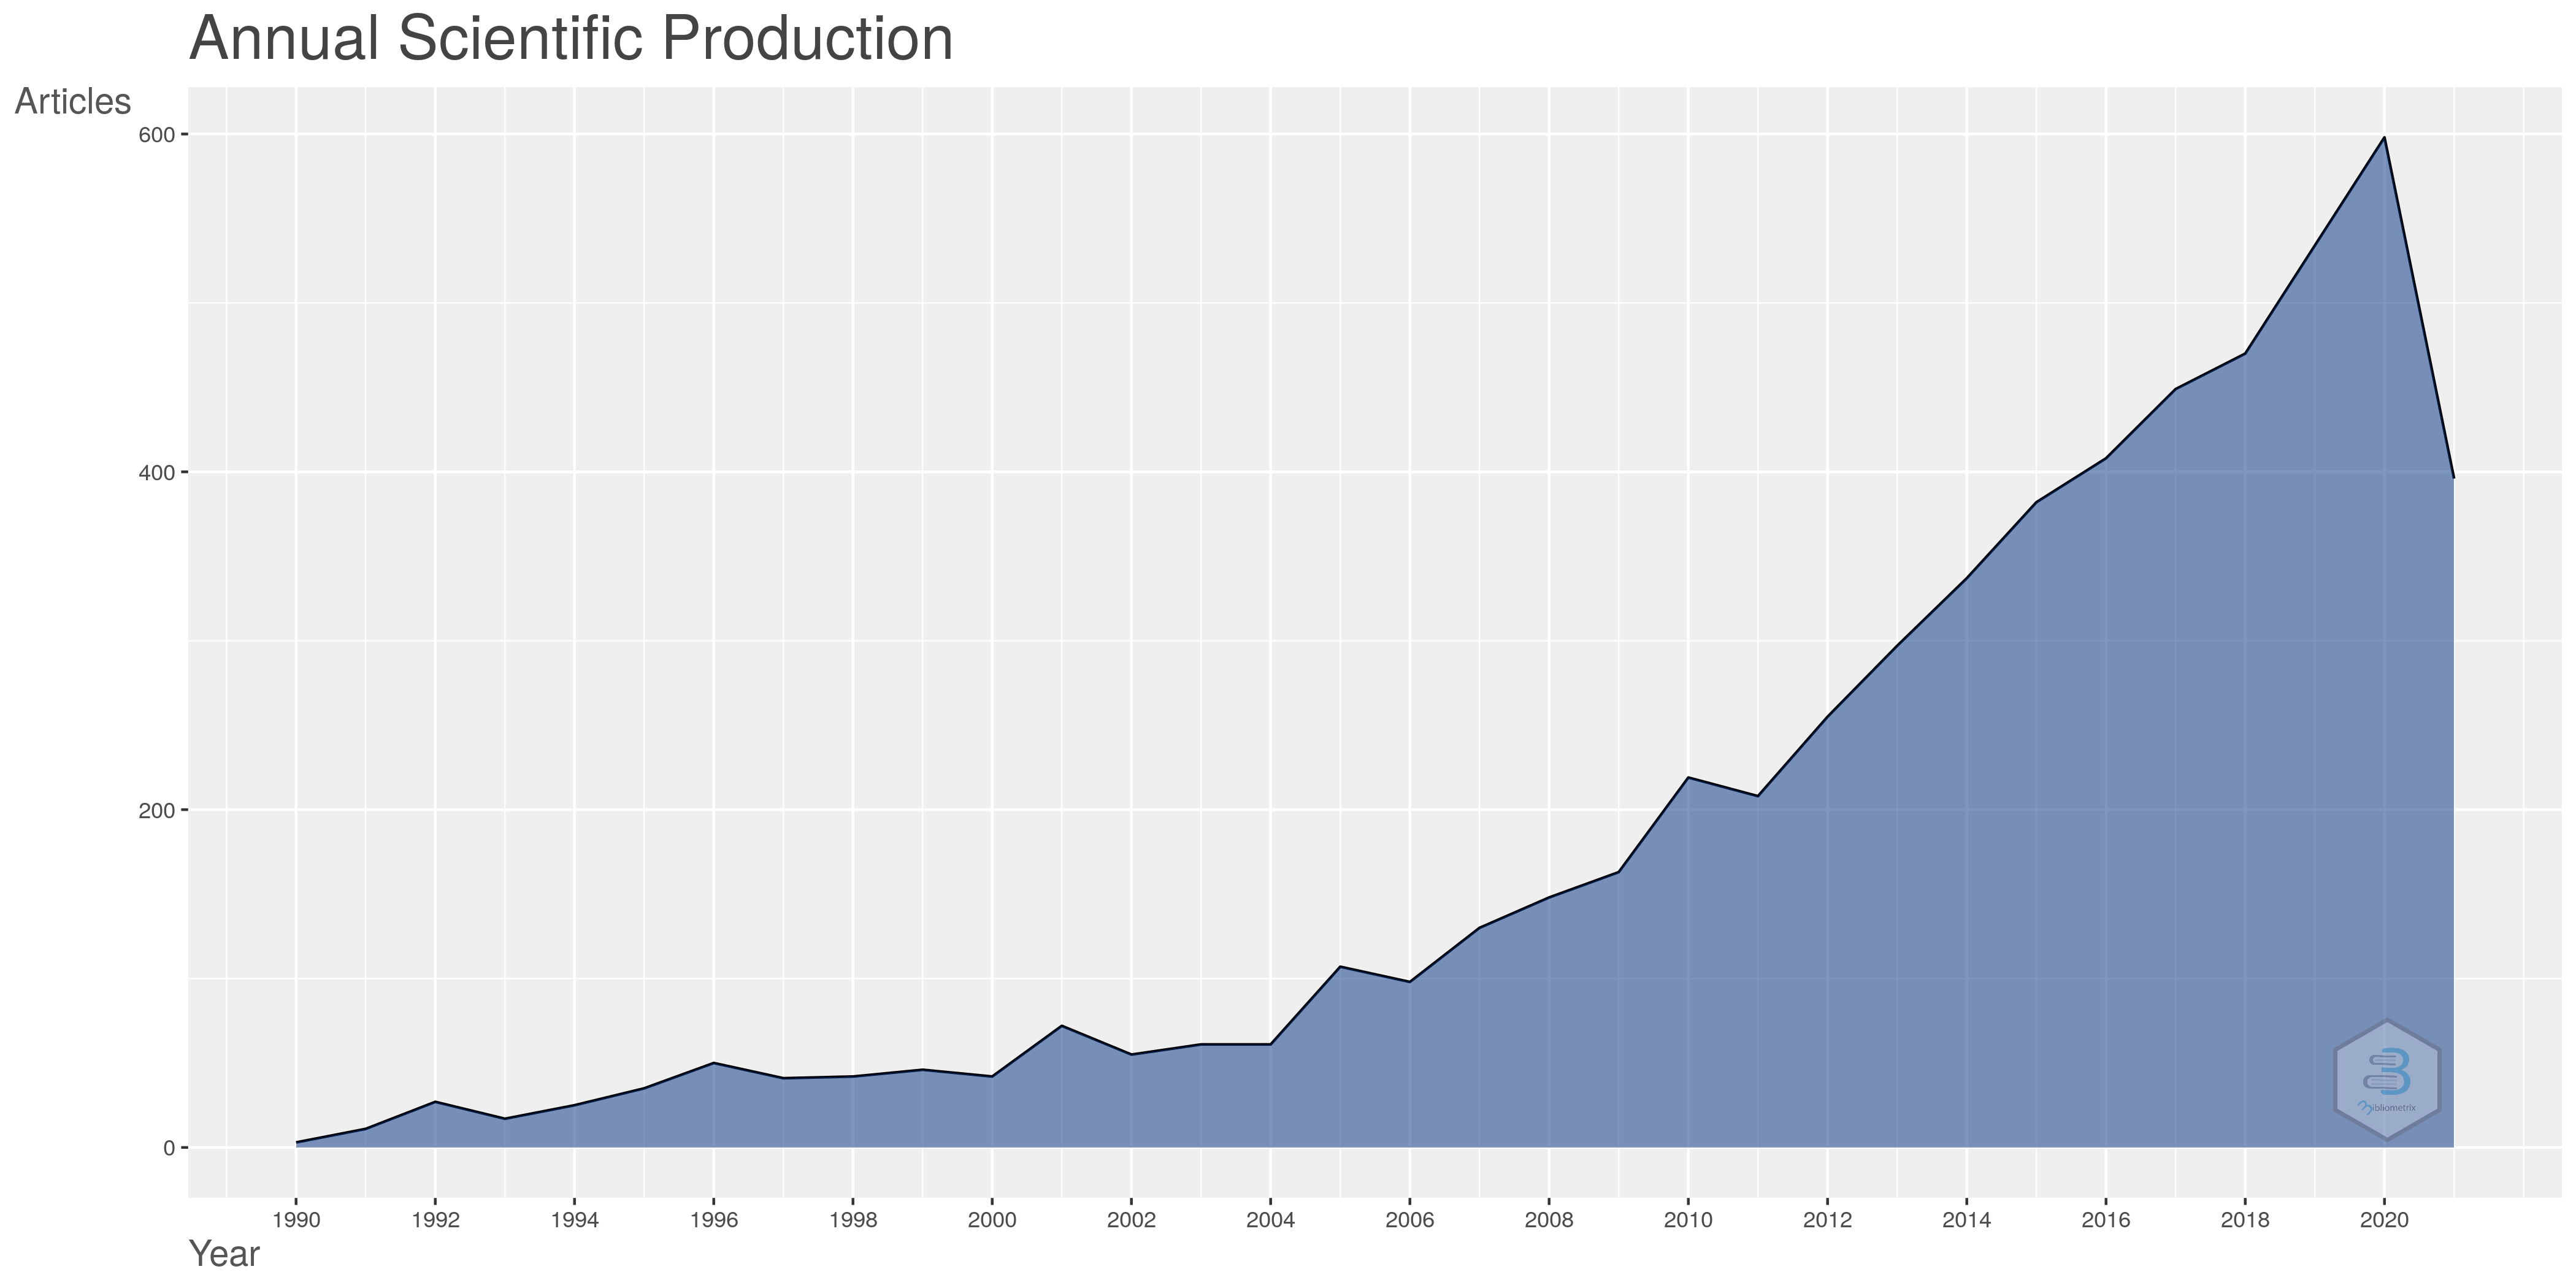
\includegraphics[width=1\textwidth]{experiments/jhcf/PesqBibliogr/SimulacaoMultiagente/WoS-20210803/classico-mais-citacoes/Dataset/AnnualScientificProduction-2021-08-05.png}
    \caption{Evolução da produção científica no \dataset\   MASSA@jhcf.}
    \label{fig:evol:anual:MASSA@jhcf}
\end{figure}

A figura \ref{fig:evol:anual:MASSA@jhcf} apresenta a evolução da produção científica mundial no tema de interesse, segundo o \dataset\   MASSA@jhcf. A curva mostra uma tendência de crescimento aproximadamente exponencial da quantidade de publicações, desde a primeira identificada em 1990.

O \textit{Annual Growth Rate} do \dataset\   é de 17,06\%, bem maior que a taxa média de crescimento da publicação científica mundial, de cerca de 3,3\% anuais, em 2016, como ilustra o estudo em \url{https://www.researchgate.net/publication/333972683_Dynamics_of_scientific_production_in_the_world_in_Europe_and_in_France_2000-2016}, página 23.

\subsection{Interpretação do Crescimento} A maior taxa de crescimento do \dataset\   MASSA@jhcf, bem como o seu grande volume, sugerem que o assunto em pauta desperta intenso interesse, inclusive de ordem econômica.

\subsection{Evolução das Citações}

\begin{figure}
    \centering
    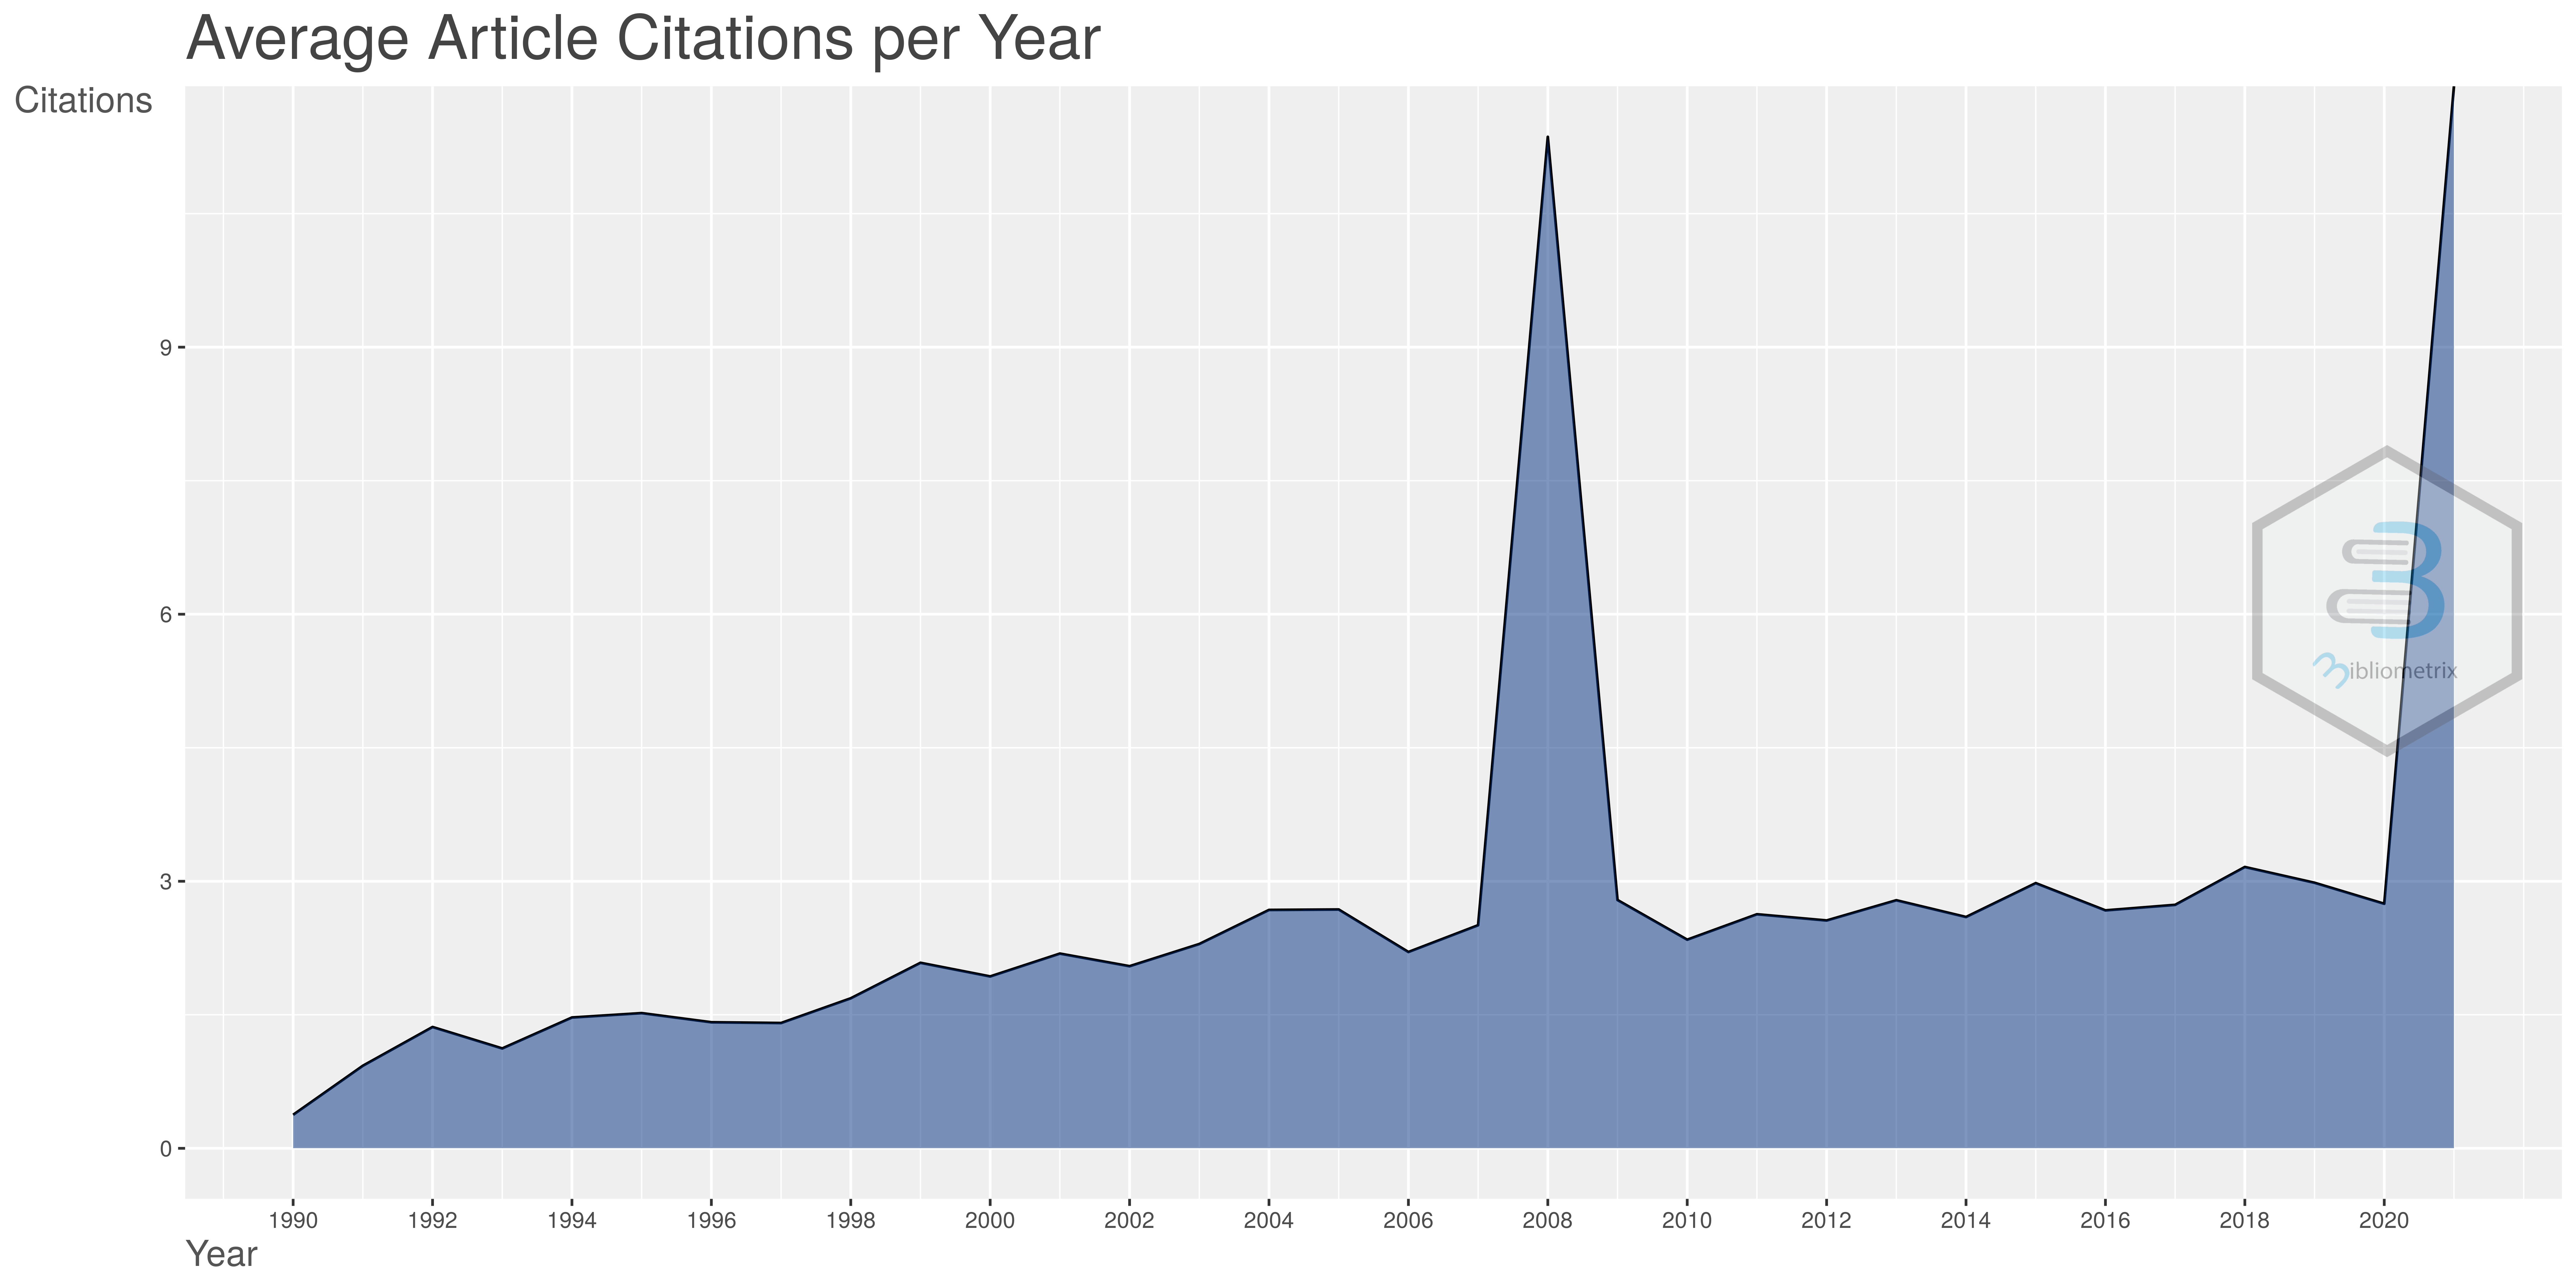
\includegraphics[width=1\textwidth]{experiments/jhcf/PesqBibliogr/SimulacaoMultiagente/WoS-20210803/classico-mais-citacoes/Dataset/AverageArticleCitationPerYear-2021-08-09.png}
    \caption{Evolução das citações ao \dataset\   MASSA@jhcf.}
    \label{fig:evol:anual:citacoes:MASSA@jhcf}
\end{figure}

A figura \ref{fig:evol:anual:citacoes:MASSA@jhcf} apresenta a evolução da média de citações aos 5.787 artigos no \dataset\   MASSA@jhcf. 
Nota-se grande estabilidade na média anual de citações, onde os artigos publicados em 1992 possuem cerca de 2 citações médias, e em 2015 (17 anos depois) o valou alterou-se apenas para três. O pico que aparece no ano de 2008 deve-se, possivelmente, à presença de um artigo do \dataset, publicado em 2008, que possui um número surpreendente grande de citações. \footnote{Note que o cálculo do número  médio de citações, nesse caso, utiliza os valores computados no tag "TC (Times Cited)", já presentes no \dataset\   obtido. Ou seja, o gráfico baseia-se no número de citações globais (externas ao \dataset\   MASSA@jhcf), e não no número de citações locais (citações a um artigo do \dataset\   feitas por alguns dos outros artigos dentro do próprio \dataset).}.

\subsection{Interpretação das Citações}
Mesmo perante um crescimento aproximadamente exponencial no volume de publicações, a ocorrência de um crescimento nas citações médias ao longo dos anos sugere que os artigos do \dataset\   possuem uma tendência de crescimento no tamanho da bibliografia citada, bem como também despertam grande interesse dos cientistas nas demais áreas do conhecimento (já que se trata de citações globais).

\subsection{\textit{Three-Field Plots (Sankey diagram)} \label{MASSA:Sankey}}

As \textit{Three-Field Plots (Sankey diagram)} (plotagens do tipo ``Três Campos'') apresentam afinidades entre três conjuntos de atributos agregados que ocorrem no \dataset. Uma plotagem do tipo Sankey busca mostrar os principais fluxos entre diferentes conjuntos de itens. \footnote{Para uma introdução ver \url{https://en.wikipedia.org/wiki/Sankey_diagram}. Para obter detalhes sobre a forma de geração e utilização desse gráfico, inclusive de forma interativa, veja o vídeo em \url{https://www.youtube.com/watch?v=jBb1iha6-sg}.} 

\begin{figure}
    \centering
    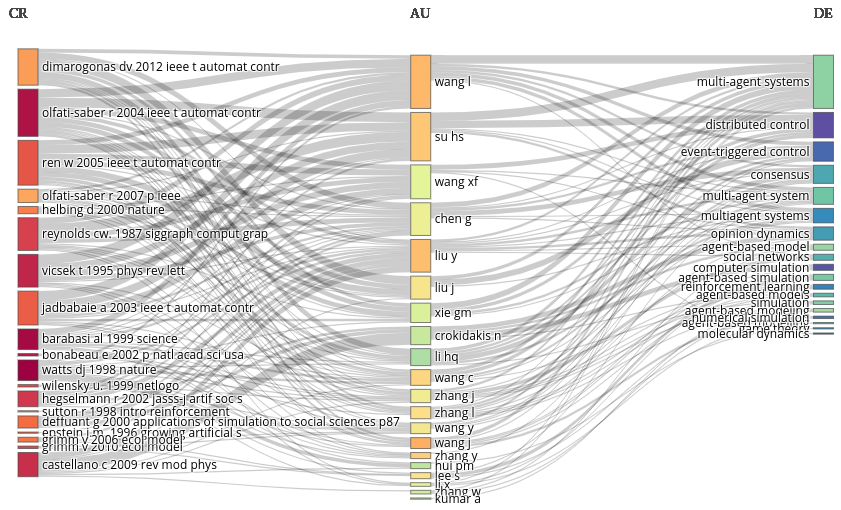
\includegraphics[angle=0,width=1\textwidth]{experiments/jhcf/PesqBibliogr/SimulacaoMultiagente/WoS-20210803/classico-mais-citacoes/Dataset/ThreeFieldPlot-AU-CR-DE-20-20-20.png}
    \caption{Plotagem ``Três Campos'' (Sankey plot) do \dataset\   MASSA@jhcf: 20 Autores, Citações e Palavras-Chave mais proeminentes.}
    \label{fig:MASSA@jhcf:ThreeFieldPlot}
\end{figure}

A figura \ref{fig:MASSA@jhcf:ThreeFieldPlot} apresenta a plotagem do tipo ``Três Campos'' do \dataset\   MASSA@jhcf, vinculando, ao centro, os 20 Autores mais proeminentes (AU), à esquerda, as 20 Citações mais frequentes (CR - Cited Records), e à direita, as 20 Palavras-Chave mais frequentes empregadas pelos autores.

\subsection{Interpretação da figura \ref{fig:MASSA@jhcf:ThreeFieldPlot}}

Os vinte autores mais relevantes, citados pelos artigos do \dataset\ MASSA, e as palavras-chave mais relevantes são aparentemente de origem asiática, mais especificamente chinesa, com base nos sobrenomes. De outra forma, a mesma origem chinesa parece não se aplicar aos trabalhos mais citados, aparentemente europeus ou norte-americanos. Isso sugere estar ocorrendo uma migração recente da produção científica, do ocidente para o oriente. 

Adicionalmente, dentre as palavras-chave (DE) não relacionadas diretamente aos termos de busca, emergem os termos \textbf{distributed control}, \textbf{event-triggered control}, \textbf{consensus} e \textbf{opinion dynamics}. Isso sugere foco das pesquisas por autores de origem chinesa no uso de simulação multiagente voltada à compreensão dos fenômenos de controle social distribuído, formação de consenso e dinâmica da opinião (pública?).

Ainda sobre a interpretação da plotagem da figura \ref{fig:MASSA@jhcf:ThreeFieldPlot}, observa-se que os artigos mais citados encontram-se publicados pelo menos 10 anos atrás, sugerindo que não houve, nos últimos 10 anos, nenhum trabalho que tenha produzido uma mudança de paradigma no tema.
A fim de melhor evidenciar as citações mais relevantes segundo o peso dos autores e palavras-chave, o gráfico da figura \ref{fig:MASSA@jhcf:ThreeFieldPlot:10-20-20} plota apenas as 10 referências citadas, para 20 autores e palavras-chave mais proeminentes.

\begin{figure}
    \centering
    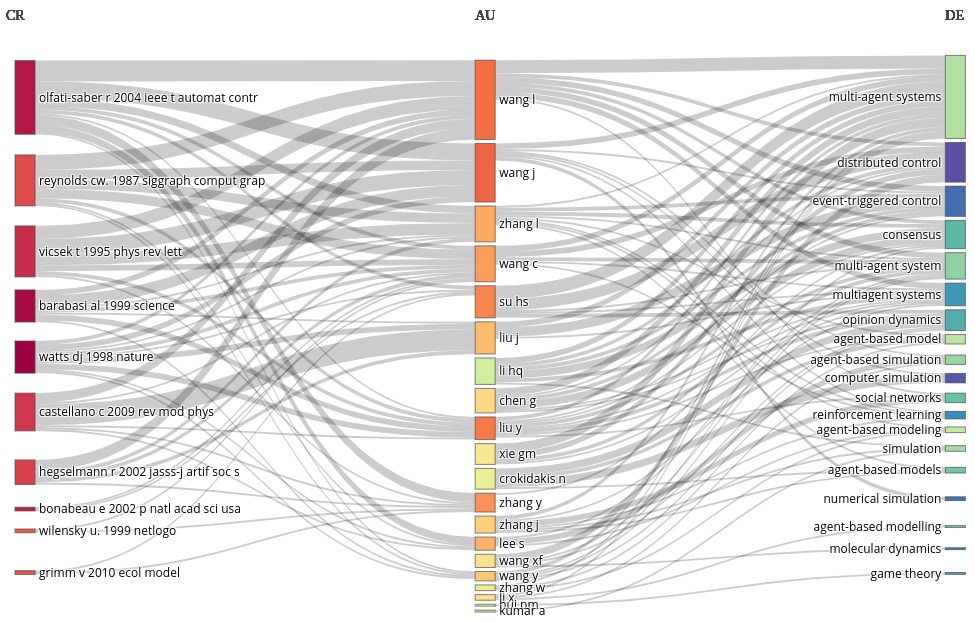
\includegraphics[angle=0,width=1\textwidth]{experiments/jhcf/PesqBibliogr/SimulacaoMultiagente/WoS-20210803/classico-mais-citacoes/Dataset/ThreeFieldPlot-AU-CR-DE-20-10-20.png}
    \caption{Plotagem ``Três Campos'' (Sankey plot) do \dataset\   MASSA@jhcf: 10 Autores, 20 Citações e Palavras-Chave mais proeminentes.}
    \label{fig:MASSA@jhcf:ThreeFieldPlot:10-20-20}
\end{figure}

\subsubsection{Autores mais relevantes\label{MASSA:Sankey:AutoresRelevantes}}

Breves comentários sobre cada um dos trabalhos mais citados serão apresentados a seguir.

\begin{itemize}
    \item  \cite{olfati-saber_consensus_2004} descrevem as propriedades algorítmicas fundamentais do ``problema do consenso'' entre agentes em redes com topologias fixas e móveis;
    \item  \cite{reynolds_flocks_1987} apresenta modelos multi-agentes para simulação gráfica do movimento de rebanhos ou agregados de animais;
    \item \cite{vicsek_novel_1995} analisam a emergência de um novo fenômeno de transição de fase em simulações de partículas com comportamento autônomo com interação biologicamente motivada, usando modelos analíticos e numéricos com uma regra de comportamento bastante simples;
    \item \cite{barabasi_emergence_1999} investigam como ocorre a emergência da distribuição livre de escala (\textit{scale-free}, uma  propriedade emergente em sistemas interativos complexos \footnote{Ver introdução em \url{https://en.wikipedia.org/wiki/Scale-free_network}.}), em redes que evoluem com base em ligação preferencial;
    \item \cite{watts_collective_1998} exploram a emergência do fenômeno ``mundo pequeno'' (\textit{small world}\footnote{Ver introdução em \url{https://en.wikipedia.org/wiki/Small-world_network}.}) formado a partir da reorganização aleatória de redes biológicas, genéticas e outras formas de redes auto-organizadas;
    \item \cite{castellano_statistical_2009} exploram de que forma as técnicas de análise e simulação já usadas na física-estatística podem ser usadas para explicar vários fenômenos sociais, tais como comportamento de multidões, dispersão social, comportamento de multidões etc. Eles apresentam as afinidades entre os dados gerados pelos modelos simulados e dados empíricos obtidos junto a sistemas sociais reais;
    \item \cite{hegselmann_opinion_2002} exploram a emergência de fenômenos de consenso, polarização e fragmentação da opinião na simulação de sociedades artificiais, descrevendo um \textit{framework} unificado para a modelagem baseada em agentes, apresentando definições matemáticas, ferramentas e teoremas;
    \item \cite{bonabeau_agent-based_2002} descreve os fundamentos da modelagem baseada em agentes para simular sistemas humanos, apresentando aplicações práticas voltadas a quatro tipos de aplicações no mundo real: \textit{''flow simulation, organizational simulation, market simulation, and diffusion simulation''};
    \item \cite{wilensky_netlogo_1999} apresentam a linguagem e ambiente de simulação NetLogo; e
    \item \cite{grimm_odd_2010} apresenta uma revisão do protocolo ODD, proposto para padronizar a descrição de modelos de simulação multiagente.
\end{itemize}

Nenhum desses 10 documentos citados está contido no \dataset\   recuperado.

%\subsection{Análises Bibliométricas: Fontes de Informação}

%\begin{figure}
%    \centering
%    \includegraphics[angle=0,width=1\textwidth]{}
%    \caption{Plotagem ``Três Campos'' (Sankey plot) do dataset MASSA@jhcf: 20 Autores, Citações e Palavras-Chave mais proeminentes.}
%    \label{fig:MASSA@jhcf:ThreeFieldPlot}
%\end{figure}

\section{Refinamento da Coleta de Dados}

No dia 03 de fevereiro de 2022, no decorrer das análises mais refinadas do \dataset\ MASSA@jhcf, identificou-se um grupo de artigos que não se encaixavam no tema de interesse, e que eram voltados para pesquisas no campo da biologia experimental e nanotecnologia. Isso sugeriu que a \query\  de busca precisaria ser reformulada, para excluir artigos que não se enquadrassem na temática desejada.
O conjunto das palavras-chave que refletia essa dissonância ficou evidente na análise da estrutura intelectual do conhecimento, do tipo \textbf{Rede de Co-ocorrências de Palavras-chave}, ilustrada no cluster em roxo, à esquerda da figura \ref{fig:MASSA@jhcf:redecoocorr-150-termos}.

\begin{figure}[htp]
    \centering
    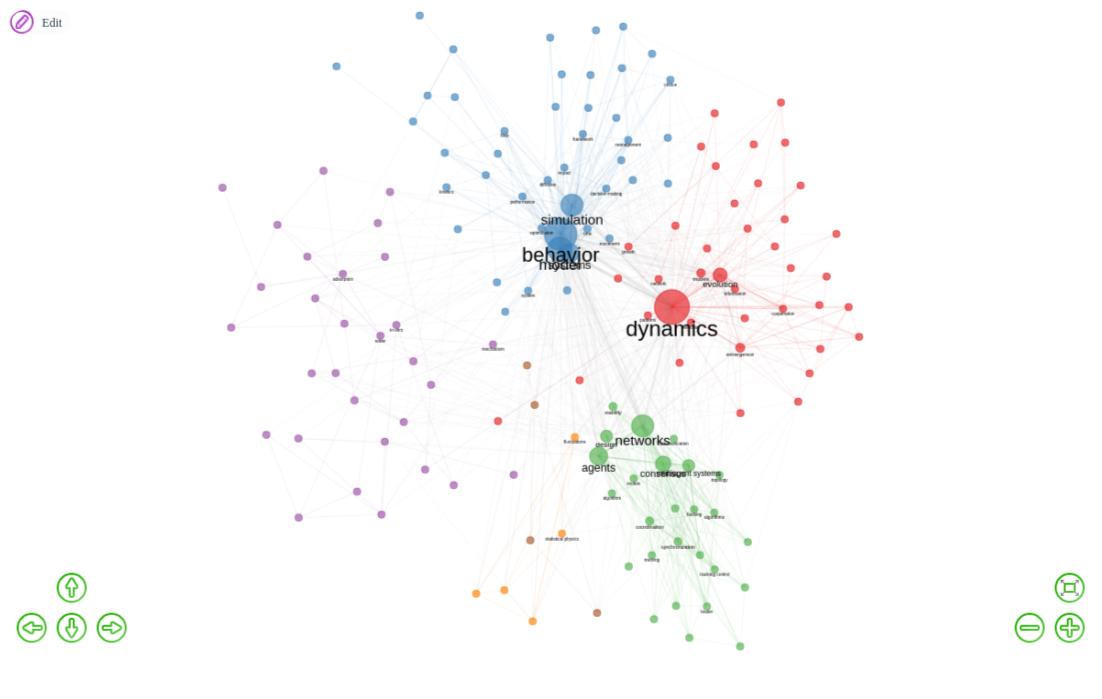
\includegraphics[clip=true,trim={9cm 0cm 7cm 0cm },width=0.6\textwidth]{experiments/jhcf/PesqBibliogr/SimulacaoMultiagente/WoS-20210803/classico-mais-citacoes/Structure-Informetric/Conceptual/Co-occurrence Network-Keywords-Plus-150-termos.png}
    \caption{Rede de co-ocorrência de palavras, com 150 termos, aplicada ao \dataset\   MASSA@jhcf.}
    \label{fig:MASSA@jhcf:redecoocorr-150-termos}
\end{figure}

As seguintes 30 palavras foram identificadas nesse \textit{cluster}:
in-vitro,
adsorption,
mechanism,
water,
force-field,
molecular-dynamics,
binding,
simulations,
nanoparticles,
bubbles,
derivatives,
temperature,
in-vivo,
mathematical-model,
oscillations,
scattering,
cancer,
contrast agents,
expression,
protein,
activation,
delivery,
surface,
removal,
acid,
agent,
reduction,
aqueous-solution,
degradation,
expectations.

Ficou evidente, pela interpretação do significado da maioria desses termos, que tais artigos não tratavam de simulação de fenômenos sociais. Isso sugere que a query está com problemas de precisão, isso é, muitos registros recuperados não atendem à necessidade de informação do pesquisador. 

Algumas dessas palavras foram então escolhidas para servir como indicativas de artigos fora do escopo, e introduzidas a partir da \query\  original, gerando uma nova \query, aprimorada e ilustrada nas linhas 1 a 13 da listagem \ref{query20220203}.

\lstinputlisting[numbers=left,basicstyle=\normalsize\ttfamily,caption={\query\  de busca sobre simulação multiagente de fenômenos socials, com ênfase em métodos experimentais, com escopo negativo de artigos que tratam de experimentos biológicos em vitro.},label=query20220203]
{experiments/jhcf/PesqBibliogr/SimulacaoMultiagente/WoS-20220203/query-Refinada.txt}

Além das justificativas para os termos usados entre as linhas 1 a 9, já descritas em \ref{MASSA:query},  justifica-se na listagem \ref{query20220203}, a inclusão da cláusula \textit{not (
 adsoption or molecular-dynamics or force-field
 or in-vitro or nanopartic* or in-vivo
 or aqueous-solution or protein or surface)}, entre as linhas 10 e 13 da \query, pois elas irão remover artigos não se enquadram no escopo da busca desejada, por usarem uma ou mais desses termos no título, resumo ou palavras-chave do artigo.
 
Usando a nova \query\ de busca, foram recuperados, em todas as edições do Web of Science\footnote{SCI-EXPANDED, SSCI, AHCI, CPCI-S, CPCI-SSH, ESCI}, 6.935 documentos, que se encontram em
\url{https://github.com/jhcf/Comput-Experim-20212/experiments/jhcf/PesqBibliogr/SimulacaoMultiagente/ WoS-20220203/wos6935recs.txt}. Comparado ao tamanho do \dataset\ anterior, isso sugere que aproximadamente 1.000 registros não se enquadravam na necessidade de busca.
Uma nova análise dos dados recuperados é apresentada a seguir.

\section{Nova Análise dos Dados}

\subsection{Nova filtragem de registros}

Sobre os 6.935 documentos recuperados, foram  aplicados os seguintes filtros:
\begin{itemize}
    \item Remoção dos registros de documentos que não são artigos \textit{full paper}, isso é, artigos completos publicados em revistas;
%    \item Remoção dos registros de artigos científicos que não fazem parte do \textit{core} da bibliografa, segundo a Lei de Bradford.
\end{itemize}

Após os filtros aplicados (apenas um)  obteve-se um total de 4.647 registros, que doravante serão chamados de forma coletiva, de \dataset\   MASSA2@jhcf.

\subsection{Análise descritiva do \dataset\   MASSA2@jhcf}

\subsubsection{Dados Sumários Gerais}

\begin{table}[htp]
    \centering
\csvautotabular[separator=semicolon
%,filter not strcmp={\csvcolii}{}
]{experiments/jhcf/PesqBibliogr/SimulacaoMultiagente/WoS-20220203/Descritiva/MASSA2-Main-Information.csv}
    \caption{Principais dados descritivos do \dataset\   MASSA2@jhcf.}
    \label{tab:MASSA2:Main}
\end{table}

Nota-se, com os resultados da tabela \ref{tab:MASSA2:Main}, que o \dataset\   abrange um período de 32 anos de publicações (1991 a 2022), evidenciando  a publicação dos 4.647 artigos em 1.910 revistas distintas. Esses artigos tem idade média de publicação de 7.8.

Adicionalmente, o \dataset\ apresenta 157.507 referências citadas, com uma média de (157.507/4.647 = ?) 33,89 referências citadas por artigo.

14.229 autores distintos produziram os artigos, com uma média de 3,73 autores por documento.

\subsubsection{Evolução anual da produção científica}

No tema de simulação multiagente de fenômenos sociais, a evolução anual da produção científica mundial é sumarizada no gráfico da figura \ref{fig:MASSA2:Annual-Scientific-Production}.

\begin{figure}
    \centering
    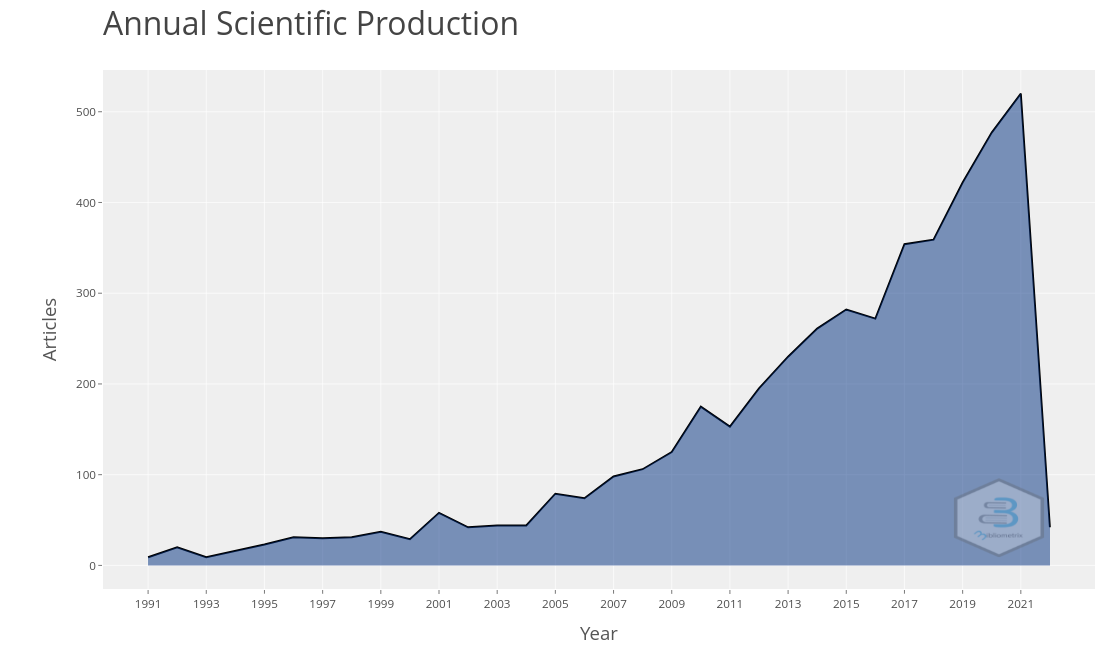
\includegraphics[width=1\textwidth]{experiments/jhcf/PesqBibliogr/SimulacaoMultiagente/WoS-20220203/Descritiva/MASSA2-Annual-Scientific-Production.png}
    \caption{Evolução da Produção Científica Anual, segundo o \dataset\ MASSA2@jhcf.}
    \label{fig:MASSA2:Annual-Scientific-Production}
\end{figure}

Entre 1991 e 2005 o crescimento de publicações era quase linear. As publicações mostram-se em ascendência forte a partir dos últimos seis anos (2015). Esse crescimento tem sido visto em várias outras áreas de conhecimento.

\subsubsection{Média de citações anuais por artigo}

O gráfico da figura \ref{fig:MASSA2:Media:Citacoes} apresenta a evolução das citações anuais médias, para os artigos do \dataset\ MASSA2@jhcf. Observa-se que há um crescimento discreto da média, onde os artigos mais recentes tendem a ser mais citados, como esperado. A redução da média no ano de 2021 deve-se, provavelmente, à insuficiência de indexação e de citação para os artigos mais recentes, tendo em vista que p ano de 2021 foi encerrado há menos de dois meses. 

\begin{figure}
    \centering
    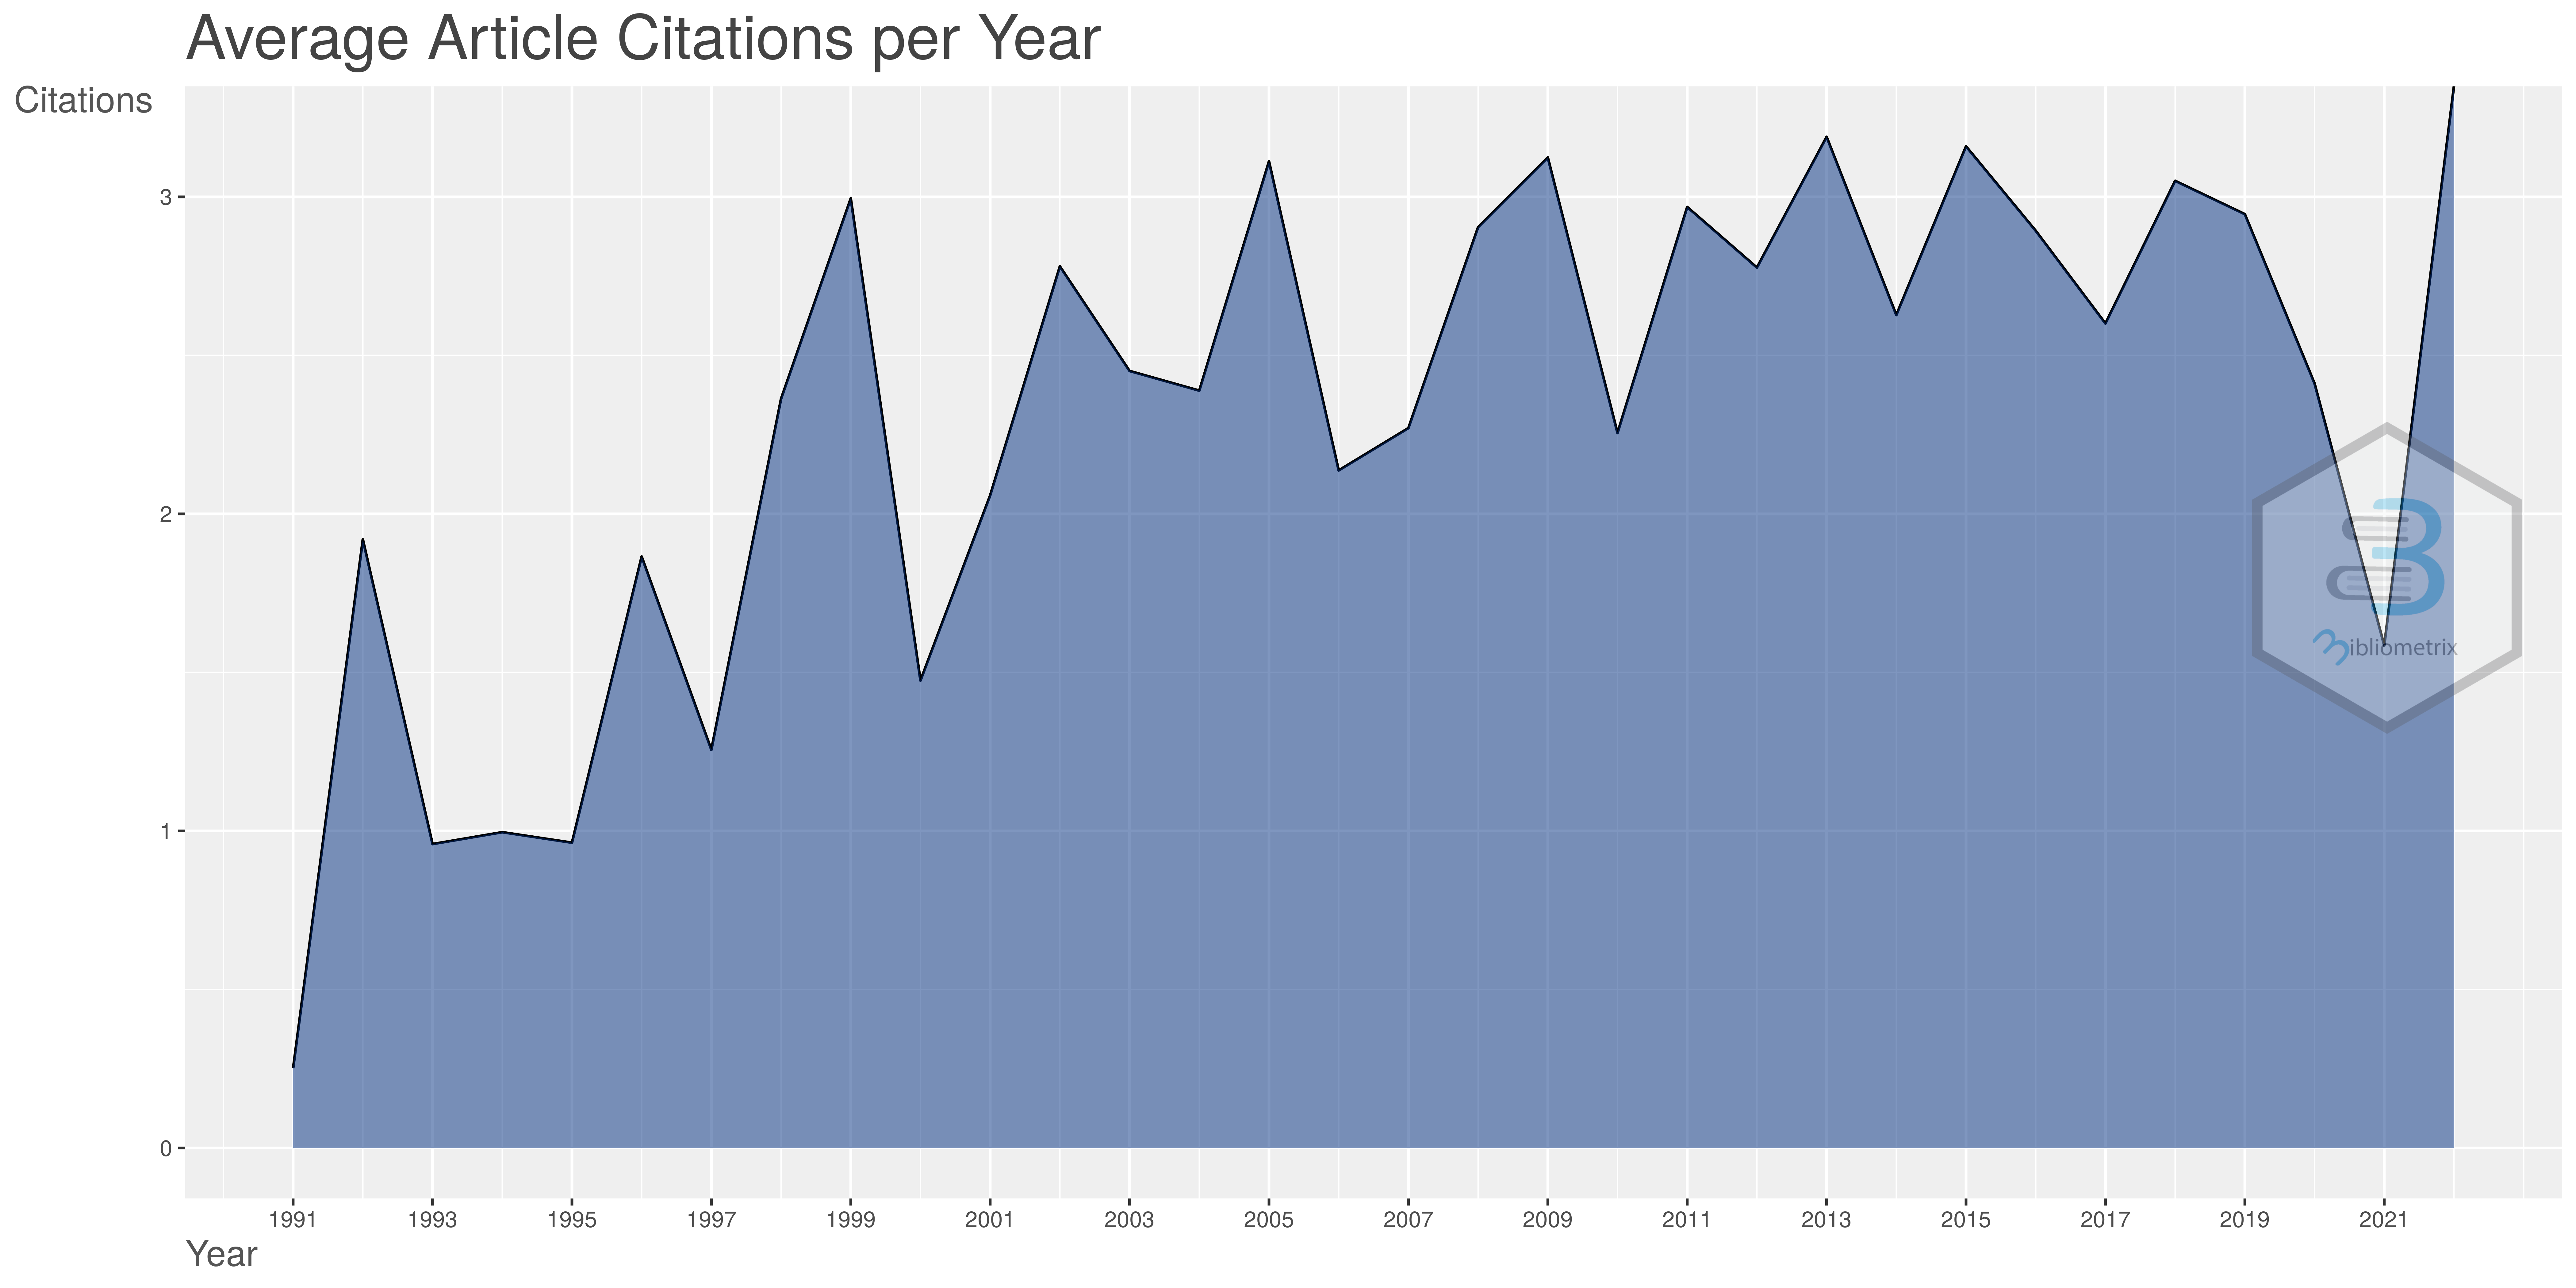
\includegraphics[width=1\textwidth]{experiments/jhcf/PesqBibliogr/SimulacaoMultiagente/WoS-20220203/Descritiva/MASSA2-Average-Citations-per-Year.png}
    \caption{Média de citações para cada artigo do \dataset\ MASSA2@jhcf, conforme o ano de publicação}
    \label{fig:MASSA2:Media:Citacoes}
\end{figure}

Para que melhor se compreenda como foi produzido o gráfico, a tabela \ref{tab:MASSA2:Media:Citacoes} apresenta parcialmente os dados de citação anual para os artigos do \dataset\ MASSA2@jhcf. A título de exemplo, nota-se que no \dataset\ foram encontrados 9 artigos publicados no ano de 1991, tendo sido cada artigo citado, em média, aproximadamente 31,4 vezes. Dado que esses artigos já tem 31 anos citáveis, obtém-se uma média de 1,01 citações anuais, aproximadamente.

\begin{table}[htp]
    \centering
\csvautotabular[separator=semicolon
%,filter not strcmp={\csvcolii}{}
]{experiments/jhcf/PesqBibliogr/SimulacaoMultiagente/WoS-20220203/Descritiva/MASSA2-Average-Citations-per-Year.csv}
    \caption{Dados parciais de citação anual para os artigos do \dataset\   MASSA2@jhcf.}
    \label{tab:MASSA2:Media:Citacoes}
\end{table}

\subsubsection{Diagramas de Sankey (\textit{three fields plots})} 

A fim de apresentar mais alguns dados sumários gerais sobre  o \dataset, as figuras \ref{fig:MASSA2:Sankey:CR-AU-DE} e \ref{fig:MASSA2:Sankey:SO:DE:AU_UN} apresentam plotagens do tipo 
\textit{three fields plots}, também conhecidas pelo nome de Diagramas de Sankey \citep{riehmann_interactive_2005}, que possibilitam várias combinações de afinidades mais evidentes entre as diversas colunas dos registros do \dataset.

A primeira plotagem, figura \ref{fig:MASSA2:Sankey:CR-AU-DE}, apresenta as afinidades mais evidentes entre 15 Autores (centro), 15 Palavras-chave (direita) e 15 Referências citadas (esquerda). Ao centro, observa-se que os autores mais evidentes, segundo a técnica apresentada, tem origem asiática, a julgar pelos nomes. 

As 15 palavras-chave mais evidentes sugerem que o \dataset\ possui artigos que refletem a busca sobre o tema desejado, mas que há muitas palavras distintas que representam o mesmo conceito, como as a seguir listadas:
\begin{enumerate}
    \item multi-agent systems;
    \item multiagent system;
    \item multiagent system; 
    \item agent-based model;  
    \item agent-based models;
    \item agent-based modeling;
    \item agent-based simulation;
\end{enumerate}

As cinco palavras a seguir sugerem, o que pode ser comprovado com o aprofundamento desse estudo bibliográfico, que o estado da arte no tema busca atualmente respostas, ou possui fundamentos nas seguintes questões:
\begin{description}
    \item [event-triggered control] Como eventos disparadores exercem  controle sobre o comportamento (coletivo) de grupos sociais?
    \item [consensus] Como usar simulação multi-agente para entender o surgimento de consenso em grupos sociais?
    \item [opinion dynamics] Como usar simulação multi-agente para entender a dinâmica de opiniões que se formam em grupos sociais?
    \item [social networks] Como os métodos da análise de redes sociais podem ser usados no tema da simulação multiagente?
    \item [reinforcement learning] Como usar os métodos e técnicas de aprendizagem por reforço em simulação multiagente?
    \item [game theory] Como usar os métodos e técnicas da teoria dos jogos em simulação multiagente?
\end{description}

Algumas das referências citadas, apresentadas à esquerda do gráfico, devem evidenciar a pertinência das questões acima sugeridas, a ser comprovado até o final do estudo. 

\begin{figure}
    \centering
    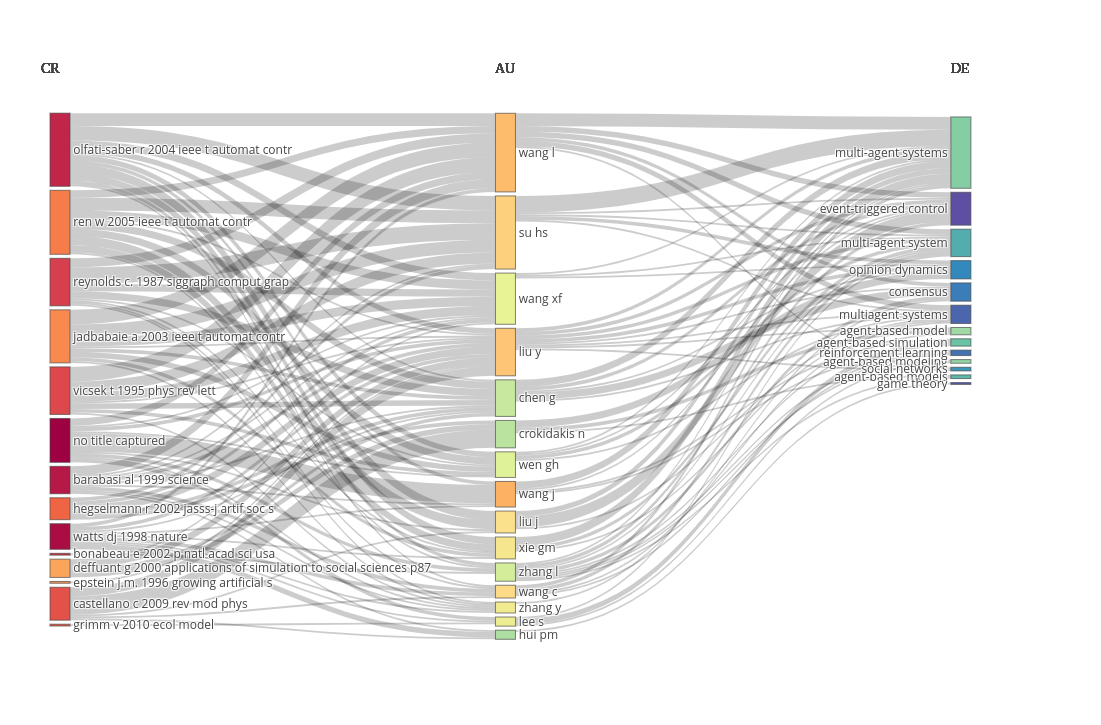
\includegraphics[angle=90,width=1\textwidth,height=0.9\textheight]{experiments/jhcf/PesqBibliogr/SimulacaoMultiagente/WoS-20220203/Descritiva/MASSA2-Three-Fields-Plot-CR-AU-DE.png}
    \caption{Diagrama Sankey, relacionando as afinidades mais evidentes entre Autores (centro), Palavras-chave (direita) e Referências citadas (esquerda).}
    \label{fig:MASSA2:Sankey:CR-AU-DE}
\end{figure}

A segunda plotagem, figura \ref{fig:MASSA2:Sankey:SO:DE:AU_UN}, apresenta as afinidades mais evidentes entre 15 revistas (esquerda), 15 palavras-chave (centro) e 15 instituições de filiação dos autores (direita). Com base na técnica usada, fica evidente a proeminência dos seguintes \textit{journals} sobre os demais, sendo apresentado um breve trecho do foco de cada revista, extraído da página online da revista:
\begin{itemize}
    \item JASSS: The Journal of Artificial Societies and Social Simulation. \textit{\small  is an interdisciplinary journal for the exploration and understanding of social processes by means of computer simulation. Since its first issue in 1998, it has been a world-wide leading reference for readers interested in social simulation and the application of computer simulation in the social sciences.}. Fonte \url{https://www.jasss.org/admin/about.html};
    \item PHYSICA A-STATISTICAL MECHANICS AND ITS APPLICATIONS. \textit{\small ... publishes research in the field of statistical mechanics and its applications. Statistical mechanics sets out to explain the behaviour of macroscopic systems, or the large scale, by studying the statistical properties of the microscopic or nanoscopic constituents. Applications of the concepts and techniques of statistical mechanics include: applications to physical and physiochemical systems such as solids, liquids and gases, interfaces, glasses, colloids, complex fluids, polymers, complex networks, applications to economic and social systems (e.g. socio-economic networks, financial time series, agent based models, systemic risk, market dynamics, computational social science, science of science, evolutionary game theory, cultural and political complexity), and traffic and transportation (e.g. vehicular traffic, pedestrian and evacuation dynamics, network traffic, swarms and other forms of collective transport in biology, models of intracellular transport, self-driven particles), as well as biological systems (biological signalling and noise, biological fluctuations, cellular systems and biophysics); and other interdisciplinary applications such as artificial intelligence (e.g. deep learning, genetic algorithms or links between theory of information and thermodynamics/statistical physics.).}. Fonte: \url{https://www.journals.elsevier.com/physica-a-statistical-mechanics-and-its-applications};
    \item IEEE ACCESS. \textit{\small ... is a multidisciplinary, all-electronic archival journal, continuously presenting the results of original research or development across all IEEE’s fields of interest. Supported by article processing charges (APC), its hallmarks are a rapid peer review and publication process of 4 to 6 weeks, with open access to all readers.}. Fonte: \url{https://ieeeaccess.ieee.org/about-ieee-access/learn-more-about-ieee-access/}
\end{itemize} 

\begin{figure}
    \centering
    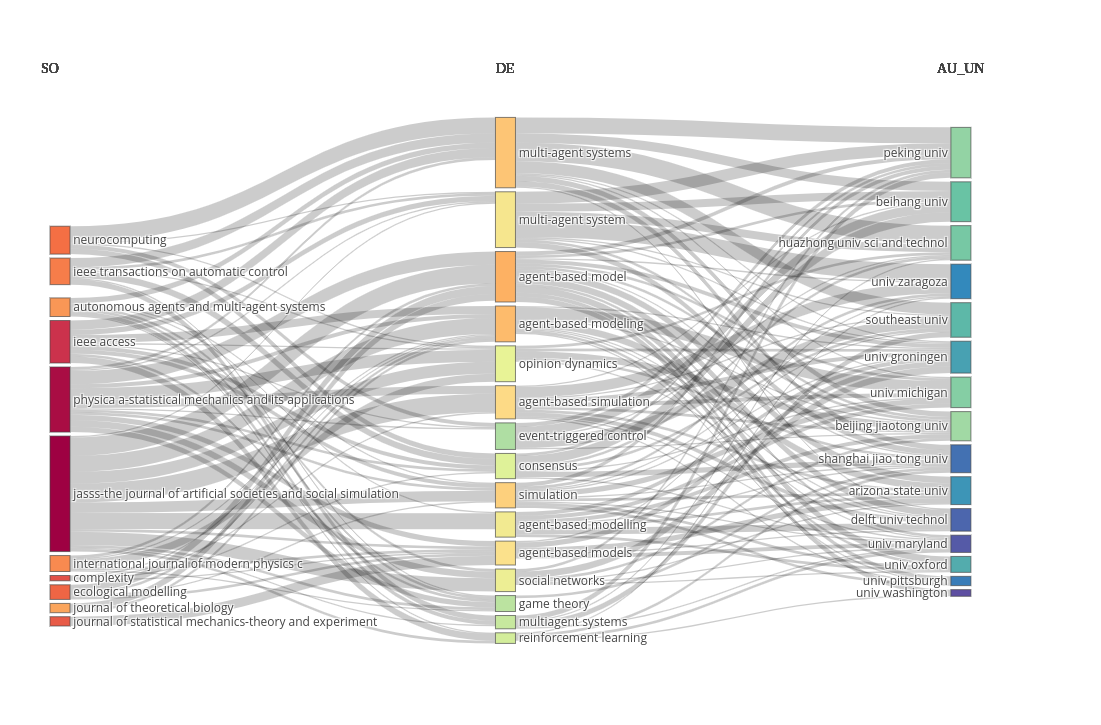
\includegraphics[angle=90,width=1\textwidth,height=0.9\textheight]{experiments/jhcf/PesqBibliogr/SimulacaoMultiagente/WoS-20220203/Descritiva/MASSA2-Three-Fields-Plot-SO:DE:AU_UN.png}
    \caption{Diagrama Sankey, relacionando as afinidades mais evidentes entre revistas (esquerda), palavras-chave (centro) e instituição de filiação dos autores (direita).}
    \label{fig:MASSA2:Sankey:SO:DE:AU_UN}
\end{figure}

Observa-se, com base no escopo declarado de cada uma das revistas, que a revista JASSS é bem enquadrada no escopo da busca, enquanto que a revista IEEE Access não tem relação direta com o tema. Já a revista Physica A aborda o tema de forma mais ampla do que o buscado, com ênfase em métodos da mecânica estatística, que não são os únicos possíveis de serem empregados.
Os nomes das demais 8 revistas, apresentadas no diagrama, são os seguintes:
\begin{enumerate}
    \item NEUROCOMPUTING \textit{\small  ... welcomes theoretical contributions aimed at winning further understanding of neural networks and learning systems, including, but not restricted to, architectures, learning methods, analysis of network dynamics, theories of learning, self-organization, biological neural network modelling, sensorimotor transformations and interdisciplinary topics with artificial intelligence, artificial life, cognitive science, computational learning theory, fuzzy logic, genetic algorithms, information theory, machine learning, neurobiology and pattern recognition.}. Fonte: \url{https://www.journals.elsevier.com/neurocomputing};
    \item IEEE TRANSACTIONS ON AUTOMATIC CONTROL \textit{\small publishes high-quality papers on the theory, design, and applications of control engineering.  Two types of contributions are regularly considered: 
1) Papers:  Presentation of significant research, development, or application of control concepts. 
2) Technical Notes and Correspondence:  Brief technical notes, comments on published areas or established control topics, corrections to papers and notes published in the Transactions.
In addition, special papers (tutorials, surveys, and perspectives on the theory and applications of control systems topics) are solicited. }. Fonte: \url{https://ieeexplore.ieee.org/xpl/aboutJournal.jsp?punumber=9};
    \item AUTONOMOUS AGENTS AND MULTI-AGENT SYSTEMS \textit{\small is the official journal of the International Foundation for Autonomous Agents and Multi-Agent Systems. It provides a leading forum for disseminating significant original research results in the foundations, theory, development, analysis, and applications of autonomous agents and multi-agent systems. Coverage in Autonomous Agents and Multi-Agent Systems includes, but is not limited to:
Agent decision-making architectures and their evaluation, including: cognitive models; knowledge representation; logics for agency; ontological reasoning; planning (single and multi-agent); reasoning (single and multi-agent)
Cooperation and teamwork, including: distributed problem solving; human-robot/agent interaction; multi-user/multi-virtual-agent interaction; coalition formation; coordination
Agent communication languages, including: their semantics, pragmatics, and implementation; agent communication protocols and conversations; agent commitments; speech act theory
Ontologies for agent systems, agents and the semantic web, agents and semantic web services, Grid-based systems, and service-oriented computing
Agent societies and societal issues, including: artificial social systems; environments, organizations and institutions; ethical and legal issues; privacy, safety and security; trust, reliability and reputation
Agent-based system development, including: agent development techniques, tools and environments; agent programming languages; agent specification or validation languages
Agent-based simulation, including: emergent behavior; participatory simulation; simulation techniques, tools and environments; social simulation
Agreement technologies, including: argumentation; collective decision making; judgment aggregation and belief merging; negotiation; norms
Economi c paradigms, including: auction and mechanism design; bargaining and negotiation; economically-motivated agents; game theory (cooperative and non-cooperative); social choice and voting
Learning agents, including: computational architectures for learning agents; evolution, adaptation; multi-agent learning.
Robotic agents, including: integrated perception, cognition, and action; cognitive robotics; robot planning (including action and motion planning); multi-robot systems.
Virtual agents, including: agents in games and virtual environments; companion and coaching agents; modeling personality, emotions; multimodal interaction; verbal and non-verbal expressiveness
Significant, novel applications of agent technology
Comprehensive reviews and authoritative tutorials of research and practice in agent systems
Comprehensive and authoritative reviews of books dealing with agents and multi-agent systems.
Official journal of the International Foundation for Autonomous Agents and Multi-Agent Systems.
Covers the foundations, theory, development, analysis, and applications of autonomous agents and multi-agent systems.
Presents comprehensive reviews and authoritative tutorials of research and practice in agent systems.}. Fonte: \url{https://www.springer.com/journal/10458};
    \item INTERNATIONAL JOURNAL OF MODERN PHYSICS C \textit{\small is a journal dedicated to Computational Physics and aims at publishing both review and research articles on the use of computers to advance knowledge in physical sciences and the use of physical analogies in computation. Topics covered include: algorithms; computational biophysics; computational fluid dynamics; statistical physics; complex systems; computer and information science; condensed matter physics, materials science; socio- and econophysics; data analysis and computation in experimental physics; environmental physics; traffic modelling; physical computation including neural nets, cellular automata and genetic algorithms.}. Fonte: \url{https://www.worldscientific.com/page/ijmpc/aims-scope};
    \item COMPLEXITY \textit{\small The purpose of Complexity is to report important advances in the scientific study of complex systems. Complex systems are characterized by interactions between their components that produce new information — present in neither the initial nor boundary conditions — which limit their predictability. Given the amount of information processing required to study complexity, the use of computers has been central to complex systems research. Concepts relevant to Complexity include:
    Adaptability, robustness, and resilience;
    Complex networks;
    Criticality;
    Evolution and emergent behaviour;
    Nonlinear dynamics;
    Pattern formation;
    Self-organization.
Methods used within the scientific study of complex systems frequently include:
    Agent-based modelling;
    Analytical methods;
    Cellular automata;
    Computational methods;
    Data science;
    Game theory;
    Machine learning;
    Statistical mechanics.
Applications of complex systems may be related to the following disciplines, among others:
Computational social science;    Digital epidemiology;
    Ecology;
    Economics;
    Engineering;
    Socio-technical systems;
    Statistical linguistics;
    Systems biology;
    Urban systems.}. Fonte: \url{https://www.hindawi.com/journals/complexity/about/};
    \item ECOLOGICAL MODELLING \textit{\small publishes new mathematical models and systems analysis for describing ecological processes, and novel applications of models for environmental management.
We welcome research on process-based models embedded in theory with explicit causative agents and innovative applications of existing models. And because applications can help refine models and propose new directions for research, the journal publishes both to help foster reproducibility and utility.Human activity and well-being are dependent on and integrated with the functioning of ecosystems and the services they provide. We aim to understand these basic ecosystem functions using mathematical and conceptual modelling, systems analysis, thermodynamics, computer simulations, and ecological theory, and look to a wide spectrum of applications ranging from basic ecology to human ecology to socio-ecological systems. The journal welcomes original research articles, review articles, viewpoint articles and short communications.}. Fonte: \url{https://www.journals.elsevier.com/ecological-modelling};
    \item JOURNAL OF THEORETICAL BIOLOGY \textit{\small is the leading forum for theoretical perspectives that give insight into biological processes. It covers a very wide range of topics and is of interest to biologists in many areas of research, including:
Brain and Neuroscience;
Cancer Growth and Treatment;
Cell Biology;
Developmental Biology;
Ecology;
Evolution;
Immunology;
Infectious and non-infectious Diseases;
Mathematical, Computational, Biophysical and Statistical Modeling;
Microbiology, Molecular Biology, and Biochemistry;
Networks and Complex Systems;
Physiology;
Pharmacodynamics;
Animal Behavior and Game Theory}. Fonte: \url{https://www.journals.elsevier.com/journal-of-theoretical-biology};
    \item JOURNAL OF STATISTICAL MECHANICS-THEORY AND EXPERIMENT \textit{\small is targeted to a broad community interested in different aspects of statistical physics, which are roughly defined by the fields represented in the conferences called 'Statistical Physics'. Submissions from experimentalists working on all the topics which have some 'connection to statistical physics are also strongly encouraged.
The journal covers different topics which correspond to the following keyword sections:
Quantum statistical physics, condensed matter, integrable systems;
Classical statistical mechanics, equilibrium and non-equilibrium;
Disordered systems, classical and quantum;
Interdisciplinary statistical mechanics;
Biological modelling and information}. Fonte: \url{https://iopscience.iop.org/journal/1742-5468/page/about_the_journal}.
\end{enumerate}
Considerando a possibilidade de pertinência da questão ecológica ao tema dos sistemas multi-agentes, todos os \textit{journals} identificados apresentam pertinência às perguntas de pesquisa formuladas. 

Acerca das instituições de filiação dos autores, nota-se que 1/3 delas é localizada na china, 1/3 nos EUA, e o restante na Europa e Austrália. É provável que muitos pesquisadores de origem chinesa trabalhem em universidades fora da china, no tema do \dataset.


\subsection{Medidas bibliométricas}

As medidas bibliométricas propriamente ditas, relativas ao \dataset\ MASSA2@jhcf, serão exploradas nesta subseção, e são organizadas em três conjuntos:
\begin{description}
    \item [Relativas às Fontes de Informação] Uma vez que foram consideradas apenas as publicações em revistas, todas as fontes de informação mensuradas serão revistas científicas, ou \textit{journals}. As principais medidas são de impacto das fontes, mensuradas com base no número de citações que os artigos publicados nas revistas obtiveram de outras publicações, possivelmente feitas em outras fontes de informação, como outras revistas, seções de livros, artigos de conferência etc. As citações são registradas pelas organizações que fazem indexação de artigos, como a Web of Science e SCOPUS;
    \item [Relativas aos Autores] Sempre que um artigo publicado por um ou mais autores e também indexado por uma organização (Web of Science,  SCOPUS etc), é citado em um outro artigo também indexado por essa mesma organização, então é feita a anotação de uma citação ao mesmo, e o impacto potencial desse autor sobre a ciência é atestado pelo valor mais alto da citação do conjunto de seus artigos indexados. Várias métricas (índice H, G, M etc) podem ser derivadas dessa medida (quantidade de citações), e são exploradas tanto em relação aos autores como em relação às revistas onde esses artigos foram publicados;
    \item [Relativas aos Documentos] Cada citação adicional a  um documento (artigo de revista, de conferência, livro, ou  capítulo de livro) é um indicador do impacto do documento em si, que evidencia a sua importância. Além das citações, a ocorrência de palavras dentro dos documentos, inclusive ordenada pelo tempo, também produz indicadores numéricos (métricas) relevantes para analisar a importância do documento em relação a outros. 
\end{description}

Essas medidas serão apresentadas a seguir.

\subsubsection{Bibliometrias aplicadas aos documentos (Artigos científicos) no \dataset}

\paragraph{Citações globais aos artigos no \dataset}

Cada registro recuperado no \dataset\ apresenta um conjunto de informações, dentre as quais pode constar a quantidade de vezes que uma citação ao mesmo foi registrada no índice do WoS, desde que no momento da extração seja feita essa solicitação (\textit{TC - Times Cited}).
A tabela \ref{tab:MASSA2:GlobalCitations} apresenta a lista dos 25 artigos do \dataset, que foram mais citados, ordenados de forma decrescente pelo número global de citações do artigo, nos índices da WoS. Para ada artigo é apresentada a referencia abreviada, o DOI e a quantidade de vezes que ele foi citado globalmente (no índice do WoS). Para recuperar a página do artigo deve-se abrir uma url prefixada com \url{http://doi.org/}, e informar o valor do DOI indicado, por exemplo \url{http://doi.org/10.1109/TAC.2008.2010897} levará à página do artigo mais citado, cujo título é ``Flocking of Multi-Agents With a Virtual Leader''.

\begin{table}[htp]
    \centering
\footnotesize
\csvreader[tabular = |r|l|l|r|,
separator=semicolon
%,filter not strcmp={\csvcolii}{},
, table head = \hline\hline \# & Artigo (Referência Abreviada) & DOI (Digital Object Identifier) & Tot.Cit.\\ \hline\hline,
table foot = \hline\hline
]{experiments/jhcf/PesqBibliogr/SimulacaoMultiagente/WoS-20220203/Metricas/Documentos/MASSA2-Most-Global-Cited-Documents.csv}{Paper=\paper, DOI=\doi,Total Citations=\totcit}{ \thecsvrow & {\tiny\paper} & {\tiny \doi} & \totcit}

    \caption{25 artigos mais citados globalmente no \dataset\ MASSA2@jhcf.}
    \label{tab:MASSA2:GlobalCitations}
\end{table}

Após a visitação do resumo do texto de vários dos documentos citados, percebe-se que não refletem bem o foco do \dataset, o que se justifica pelo fato de que esses documentos são os de maior citação global, e não necessariamente os que tem maior citação local ao \dataset. Dessa forma, procede-se à próxima análise.

\paragraph{Citações locais aos artigos no \dataset}

Cada registro recuperado no \dataset\ apresenta um conjunto de informações, dentre as quais consta a lista das citações feitas a outros documentos, nas seção bibliografia. O Bibliometrix computa de forma aproximada a quantidade de vezes que cada artigo do \dataset\ foi citado por outros artigos do mesmo \dataset, construindo uma tabela das maiores citações locais, que provavelmente apontará para artigos com afinidade bem maior à busca efetuada.

\begin{table}[htp]
    \centering
\footnotesize
\csvreader[tabular = |r|l|l|r|r|,
separator=semicolon,
filter={\value{csvrow}<25}
%,filter not strcmp={\csvcolii}{},
, table head = \hline\hline \# & Artigo (Referência Abreviada) & DOI  & L.Cit& G.Cit\\ \hline\hline,
table foot = \hline\hline
]{experiments/jhcf/PesqBibliogr/SimulacaoMultiagente/WoS-20220203/Metricas/Documentos/MASSA2-Most-Local-Cited-Documents.csv}{Document=\paper, DOI=\doi}{ \thecsvrow & {\tiny\paper} & {\tiny \doi} & \csvcoliii & \csvcoliv}

    \caption{25 artigos mais citados localmente no \dataset\ MASSA2@jhcf.}
    \label{tab:MASSA2:LOcalCitations}
\end{table}

A lista dos artigos retornados pelo critério de citação local retornou textos bastante pertinentes ao tema da simulação multiagente de fenômenos sociais, conforme os 25 títulos a seguir listados, seguindo a ordem apresentada na tabela:
\begin{enumerate}
    \item ``Flocking of Multi-Agents With a Virtual Leader'', trabalha com simulação numérica do vôo coletivo de agentes móveis\footnote{\textit{All agents being informed and the virtual leader traveling at a constant velocity are the two critical assumptions seen in the recent literature on flocking in multi-agent systems. Under these assumptions, Olfati-Saber in a recent IEEE Transactions on Automatic Control paper proposed a flocking algorithm which by incorporating a navigational feedback enables a group of agents to track a virtual leader.... Numerical simulation demonstrates that a very small group of the informed agents can cause most of the agents to move with the desired velocity and the larger the informed group is the bigger portion of agents will move with the desired velocity. }};
    \item ``Agent-based land-use models: a review of applications'' traça importantes direcionamentos sobre o uso de simulações multiagente para resolver problemas com o uso da terra \footnote{\textit{In this paper, we review applications of agent-based land use models under the headings of (a) policy analysis and planning, (b) participatory modelling, (c) explaining spatial patterns of land use or settlement, (d) testing social science concepts and (e) explaining land use functions. The greatest use of such models so far has been by the research community as tools for organising knowledge from empirical studies, and for exploring theoretical aspects of particular systems. However, there is a need to demonstrate that such models are able to solve problems in the real world better than traditional modelling approaches. It is concluded that in terms of decision support, agent-based land-use models are probably more useful as research tools to develop an underlying knowledge base which can then be developed together with end-users into simple rules-of-thumb, rather than as operational decision support tools.}};
    \item ``Describing human decisions in agent-based models – ODD + D, an extension of the ODD protocol'' apresenta um formato descritivo para a explanação do desenvolvimento e uso de simulações multiagentes \footnote{\textit{We expand the ODD protocol to describe human decisions in ABMs.
We exemplify the new ODD + D (ODD + Decision) with a social–ecological ABM on water use.
ODD + D facilitates communication and comparison of models.}};
\item ``Event-Triggering Sampling Based Leader-Following Consensus in Second-Order Multi-Agent Systems'' aprofunda a exploração de questões similares à do primeiro artigo desta lista, sobre o problema do consenso e da importância do líder no direcionamento de um bando de agentes \footnote{\textit{In this note, the problem of second-order leader-following consensus by a novel distributed event-triggered sampling scheme in which agents exchange information via a limited communication medium is studied. Event-based distributed sampling rules are designed, where each agent decides when to measure its own state value and requests its neighbor agents broadcast their state values across the network when a locally-computed measurement error exceeds a state-dependent threshold. }};
\item MOSS S, 2008, JASSS-J ARTIF SOC S;
\item ``Agent-based modeling in marketing: Guidelines for rigor'' propõe uma orientação metodologicamente rigorosa para o desenvolvimento de modelagem de sistemas baseados em agentes para a área de \textit{marketing}, buscando melhorar a aceitação de estudos em revistas científicas dessa outra áres\footnote{\textit{Some useful examples of agent-based modeling have been published in marketing journals, but widespread acceptance of the agent-based modeling method and publication of this method in the highest-level marketing journals have been slowed by the lack of widely accepted standards of how to do agent-based modeling rigorously. We address this need by proposing guidelines for rigorous agent-based modeling. We demonstrate these guidelines, and the value of agent-based modeling for marketing research, through the use of an example. We use an agent-based modeling approach to replicate the Bass model of the diffusion of innovations, illustrating the use of the proposed guidelines to ensure the rigor of the analysis. We also show how extensions of the Bass model that would be difficult to carry out using traditional marketing research techniques are possible to implement using a rigorous agent-based approach.}};
\item ``Time series properties of an artificial stock market'' desenvolve um modelo de simulação de um mercado financeiro, e compara os resultados do modelo com dados empíricos reais desse mercado \footnote{\textit{This paper presents results from an experimental computer simulated stock market. In this market artificial intelligence algorithms take on the role of traders. They make predictions about the future, and buy and sell stock as indicated by their expectations of future risk and return. Prices are set endogenously to clear the market. Time series from this market are analyzed from the standpoint of well-known empirical features in real markets. The simulated market is able to replicate several of these phenomenon, including fundamental and technical predictability, volatility persistence, and leptokurtosis. Moreover, agent behavior is shown to be consistent with these features, in that they condition on the variables that are found to be significant in the time series tests. Agents are also able to collectively learn a homogeneous rational expectations equilibrium for certain parameters giving both time series and individual forecast values consistent with the equilibrium parameter values.}};
\item ``Empirical characterisation of agent behaviours in socio-ecological systems'' investiga uma abordagem para desenvolvimento e validação empírica de modelos baseados em agentes para a modelagem de tomada de decisão em processos sócio-ecológicos \footnote{\textit{Agent-based modelling has become an important tool to investigate socio-ecological processes. Its use is partially driven by increasing demand from decision makers to provide support for understanding the potential implications of decisions in complex situations. While one of the advantages of agent-based modelling is the ability to simulate the implications of human decision-making processes explicitly, methods for providing empirical support for the representation of the behaviour of human agents have not been structured systematically. This paper develops a framework for the parameterisation of human behaviour in agent-based models and develops twelve distinct sequences for the characterisation and parameterisation of human behaviours. Examples are provided to illustrate the most important sequences. This framework is a first step towards a guide for parameterisation of human behaviour in ABM. A structured discussion within the agent-based community is needed to achieve a more definitive guideline.}};
\item BOERO R, 2005, JASSS-J ARTIF SOC S;
\item ``Agent-based modeling of the diffusion of environmental innovations — An empirical approach'' desenvolve e faz uma validação empírica de um modelo baseado em agentes para investigar a difusão de inovações relacionadas à economia no uso de água, calibrado com dados de uma região do sul da Alemanha \footnote{\textit{This paper presents an agent-based model of the diffusion of water-saving innovations. The empirical foundation of this model is a study, which was carried out for that specific purpose. As an example case, the diffusion of three water-related innovations in Southern Germany was chosen. The model represents a real geographic area and simulates the diffusion of showerheads, toilet flushes, and rain-harvesting systems. Agents are households of certain lifestyles, as represented by the Sinus-Milieus® from commercial marketing. Agents use two different kinds of decision rules to decide upon adoption or rejection of the modeled innovations: A cognitively demanding deliberate decision rule and a very simple decision heuristic. Thus, the model integrates concepts of bounded rationality. The overall framework for decision-making is the Theory of Planned Behavior, which has been elaborated using innovation characteristics from diffusion research. The model was calibrated with empirical data stemming from a questionnaire survey and validated against independent data. Scenarios for the nearer future show that water-saving innovations will diffuse even without further promotion, and different promotion strategies that relate specifically to both innovations and lifestyles can be pointed out.}};
\item HAPPE K, 2006, ECOL SOC;
\item ``Linking agent-based models and stochastic models of financial markets'' desenvolve e valida, de forma simulada, analítica, e fundamentada em dados empíricos (Standard \& Poor 500 Index), como e por que emergem dois comportamentos típicos no coletivo dos agentes do mercado de ativos financeiros, sugerindo abordagens que poderiam alterar a ocorrência desses fenômenos   \footnote{\textit{It is well-known that financial asset returns exhibit fat-tailed distributions and long-term memory. These empirical features are the main objectives of modeling efforts using (i) stochastic processes to quantitatively reproduce these features and (ii) agent-based simulations to understand the underlying microscopic interactions. After reviewing selected empirical and theoretical evidence documenting the behavior of traders, we construct an agent-based model to quantitatively demonstrate that “fat” tails in return distributions arise when traders share similar technical trading strategies and decisions. Extending our behavioral model to a stochastic model, we derive and explain a set of quantitative scaling relations of long-term memory from the empirical behavior of individual market participants. Our analysis provides a behavioral interpretation of the long-term memory of absolute and squared price returns: They are directly linked to the way investors evaluate their investments by applying technical strategies at different investment horizons, and this quantitative relationship is in agreement with empirical findings. Our approach provides a possible behavioral explanation for stochastic models for financial systems in general and provides a method to parameterize such models from market data rather than from statistical fitting.}};
\item ``Heterogeneous bounds of confidence: Meet, discuss and find consensus!'' investiga por métodos computacionais de simulação multiagente e análise numérica, de que forma são corroborados alguns modelos teóricos de produção de consenso em situações de confiança limitada, já existentes na literatura  \footnote{\textit{Models of continuous opinion dynamics under bounded confidence show a sharp transition between a consensus and a polarization phase at a critical global bound of confidence. In this paper, heterogeneous bounds of confidence are studied. The surprising result is that a society of agents with two different bounds of confidence (open- and closed-minded agents) can find consensus even when both bounds of confidence are significantly below the critical bound of confidence of a homogeneous society. The phenomenon is shown by examples of agent-based simulation and by numerical computation of the time evolution of the agents density. The result holds for the bounded confidence model of Deffuant, Weisbuch, and others (Weisbuch et al., Complexity 2002, 7, 55–63), as well as for the model of Hegselmann and Krause (Hegselmann and Krause, Journal of Artificial Societies and Social Simulation 2002, 5, 2).}};
\item ``The "Wedding-Ring": An agent-based marriage model based on social interaction'' desenvolve e valida um modelo de simulação baseado em agentes para corroborar modelos teóricos de micro-sociológicos acerca da idade em que ocorre o casamento entre pessoas. \footnote{\textit{In this paper we develop an agent-based marriage model based on social interaction. We build an population of interacting agents whose chances of marrying depend on the availability of partners, and whose willingness to marry depends on the share of relevant others in their social network who are already married. We then let the typical aggregate age pattern of marriage emerge from the bottom-up. The results of our simulation show that micro-level hypotheses founded on existing theory and evidence on social interaction can reproduce age-at-marriage patterns with both realistic shape and realistic micro-level dynamics.}};
\item ``Agent-based simulation of affordance-based human behaviors in emergency evacuation'' investiga o uso de modelos baseados em agentes para simular o compartamento de pessoas em situação de evacuações de emergência de incêndio \footnote{\textit{ical rule-based model, (2) a statistical model, or (3) an analytical predictive model. Predicting human behaviors in complex and uncertain environments like emergency evacuation is considered almost impossible (at least NP hard) in systems theory. In this paper, we explore simulating human behaviors using affordance-based finite state automata (FSA) modeling, based on the ecological concept of affordance theory. To this end, we introduce the conceptual and generic framework of affordance-based human behavior simulation developed through our previous work. Following the generic framework, formal simulation models of affordance-based human behaviors are developed, especially for emergency evacuation, to mimic perception-based dynamic human actions interacting with emergent environmental changes, such as fire. A “warehouse fire evacuation” case is used to demonstrate the applicability of the proposed framework. The human action planning algorithms in the simulation model are developed and implemented using the Adjusted Floor Field Indicators, which represent not only the evacuee’s prior knowledge of the floor layout but the perceivable information about dynamic environmental changes. The results of our simulation study verify that the proposed framework accurately simulates human fire evacuation behavior.}};
\item ``Flocking of Multi-Agent Non-Holonomic Systems With Proximity Graphs'' desenvolve modelos de simulação multiagente para investigação do comportamento de voo coletivo em sistemas multi-agente \footnote{\textit{A multi-agent system is composed of many agents interconnected by a communication network. This paper aims to further investigate the flocking and preserving connectedness in multi-agent nonholonomic systems with proximity graphs, in which the positions and the relative distances are not available to the distributed controllers. Several sufficient conditions are derived to resolve the above problem based on the kinematic model and the dynamic model, respectively. }};
\item ``UNIVERSALITY OF THE THRESHOLD FOR COMPLETE CONSENSUS FOR THE OPINION DYNAMICS OF DEFFUANT et al.'' investiga e propõe uma regra para desenvolvimento de modelos de simulação multiagente para a questão da formação de consenso e dinâmica de opinões em sistemas multi-agente;
\item ``Agent-based model simulations of future changes in migration flows for Burkina Faso'' investiga e valida empiricamente, por meio de modelos de simulação baseados em agente, a estrutura dos fluxos migratórios em Burkina Faso \footnote{\textit{agent-based modelling offers a robust method to simulate the autonomous decision making process relating to environmental migration. The Theory of Planned Behaviour provides a basis that can be used to effectively break down the reasoning process relating to the development of a behavioural intention. By developing an agent-based model of environmental migration for Burkina Faso from the basis of a combination of such theoretical developments and data analysis we further investigate the role of the environment in the decision to migrate using scenarios of future demographic, economic, social, political, and climate change in a dryland context. We find that in terms of climate change, it can be seen that that change to a drier environment produces the largest total and international migration fluxes when combined with changes to inclusive and connected social and political governance. While the lowest international migration flows are produced under a wetter climate with exclusive and diverse governance scenarios. In summary this paper illustrates how agent-based models incorporating the Theory of Planned Behaviour can be used to project evidence based future changes in migration in response to future demographic, economic social and climate change.}};
\item ``STATISTICAL PROPERTIES AND MULTIFRACTAL BEHAVIORS OF MARKET RETURNS BY ISING DYNAMIC SYSTEMS''investiga como a simulação baseada em agente pode ser usada para modelar a formação de preços em mercados de capitais \footnote{\textit{An interacting-agent model of speculative activity explaining price formation in financial markets is considered in the present paper, which based on the stochastic Ising model and the mean field theory. The model describes the interaction strength among the agents as well as an external field, and the corresponding random logarithmic price return process is investigated. According to the empirical research of the model, the time series formed by this Ising model exhibits the bursting typical of volatility clustering, the fat-tail phenomenon, the power-law distribution tails and the long-time memory. The statistical properties of the returns of Hushen 300 Index, Shanghai Stock Exchange (SSE) Composite Index and Shenzhen Stock Exchange (SZSE) Component Index are also studied for comparison between the real time series and the simulated ones. Further, the multifractal detrended fluctuation analysis is applied to investigate the time series returns simulated by Ising model have the distribution multifractality as well as the correlation multifractality.}};
\item ``A framework for modeling payments for ecosystem services with agent-based models, Bayesian belief networks and opinion dynamics models'' desenvolve um framework para modelagem de sistemas baseados em agentes para investigar fenômenos ligados ao uso de incentivos financeiros para melhoria da sustentabilidade ambiental \footnote{\textit{We present an integrated modeling framework for simulating land-use decision making under the influence of payments for ecosystem services. The model combines agent-based modeling (ABM) with Bayesian belief networks (BBNs) and opinion dynamics models (ODM). The model endows agents with the ability to make land-use decisions at the household and plot levels. The decision-making process is captured with the BBNs that were constructed and calibrated with both qualitative and quantitative information, i.e., knowledge gained from group discussions with stakeholders and empirical survey data. To represent interpersonal interactions within social networks, the decision process is further modulated by the opinion dynamics model. The goals of the model are to improve the ability of ABM to emulate land-use decision making and thus provide a better understanding of the potential impacts of payments for ecosystem services on land use and household livelihoods. }}.
\end{enumerate}

Após essa breve análise dos 25 artigos mais citados do \dataset\ ganhou-se uma confiança de que os dados são de boa qualidade quanto à representatividade do uso de simulações multiagentes para modelagem de fenômenos sociais. Os principais fenômenos sociais investigados nesses artigos são relacionados com as ideias de:
\begin{enumerate}
    \item Formação de consenso em coletivos;
    \item Influência da liderança na formação de consensos;
    \item Gestão coletiva no uso da terra, em interfaces ecológico-sociais;
    \item Modelagem do comportamento de \textit{traders} no mercado financeiro, especialmente formação de preços;
    \item Comportamento das pessoas em situações de desastre, especialmente incêndio;
    \item Difusão de inovações em comunidades, especialmente agrícolas;
    \item Migração de populações; 
    \item Idade em que as pessoas casam; e
    \item Modelagem de marketing (uma espécie de fenômeno de difusão de inovações em rede).
\end{enumerate}

\paragraph{Referências a outros documentos (artigos, capítulos de livros etc) citados pelos artigos no \dataset}

Cada registro do \dataset\ MASSA2@jhcf contém o conjunto das referências citadas, no campo CR. A tabelas \ref{tab:MASSA2:LocalCitationsReferences} apresentada de forma sumária quais foram as 25 citações mais frequentes, sugerindo os principais documentos que contém o conhecimento mais basilar usado pelos pesquisadores nesse campo do conhecimento da simulação multiagente de fenômenos sociais. Note que os registros de muitos desses documentos poderão não estar presentes no \dataset\ MASSA2@jhcf.

\begin{table}[htp]
    \centering
\footnotesize
\csvreader[tabular = |r|l|l|r|,
separator=semicolon
%,filter not strcmp={\csvcolii}{},
, table head = \hline\hline \# & Artigo Citado & DOI & Tot.Cit.\\ \hline\hline,
table foot = \hline\hline
]{experiments/jhcf/PesqBibliogr/SimulacaoMultiagente/WoS-20220203/Metricas/Documentos/MASSA2-Most-Local-Cited-References.csv}{Cited References=\paper, DOI=\doi,Citations=\totcit}{ \thecsvrow & {\tiny\paper} & {\tiny \doi} & \totcit}

    \caption{25 referências (artigos, capítulos de livros etc) mais citadas localmente no \dataset\ MASSA2@jhcf.}
    \label{tab:MASSA2:LocalCitationsReferences}
\end{table}

Alguns desses registros serão brevemente comentados a seguir, acrescentando-se que os dez mais citados já foram descritos na plotagem Sankey em \ref{MASSA:Sankey:AutoresRelevantes}.

\begin{enumerate}
\item \textit{\textbf{Collective dynamics of ‘small-world networks'}} \citep{watts_collective_1998}, já descrito na plotagem Sankey em \ref{MASSA:Sankey:AutoresRelevantes} tem 25136 citações globais; 
\item \textit{\textbf{Consensus problems in networks of agents with switching topology and time-delays}} \citep{olfati-saber_consensus_2004}, já descrito na plotagem Sankey em \ref{MASSA:Sankey:AutoresRelevantes}, possui 8465 citações globais;

\item \textit{\textbf{Emergence of Scaling in Random Networks}}\citep{barabasi_emergence_1999}, já descrito na plotagem Sankey em \ref{MASSA:Sankey:AutoresRelevantes};

\item \textit{\textbf{Statistical physics of social dynamics}}\citep{castellano_statistical_2009}, já descrito na plotagem Sankey em \ref{MASSA:Sankey:AutoresRelevantes}; 
\item \textit{\textbf{Novel Type of Phase Transition in a System of Self-Driven Particles}} \citep{vicsek_novel_1995}, já descrito na plotagem Sankey em \ref{MASSA:Sankey:AutoresRelevantes}; 

\item \textit{\textbf{Flocks, herds and schools: A distributed behavioral model}} \citep{reynolds_flocks_1987}, já descrito na plotagem Sankey em \ref{MASSA:Sankey:AutoresRelevantes};

\item \textit{\textbf{Agent-based modeling: Methods and techniques for simulating human systems}} \citep{bonabeau_agent-based_2002}, já descrito na plotagem Sankey em \ref{MASSA:Sankey:AutoresRelevantes};

\item \textit{\textbf{Opinion dynamics and bounded confidence: models, analysis and simulation}} \citep{hegselmann_opinion_2002}, já descrito na plotagem Sankey em \ref{MASSA:Sankey:AutoresRelevantes}; 

\item \textit{\textbf{The ODD protocol: A review and first update}} \citep{grimm_odd_2010}, já descrito na plotagem Sankey em \ref{MASSA:Sankey:AutoresRelevantes};

\item \textit{\textbf{Consensus seeking in multiagent systems under dynamically changing interaction topologies}} \citep{ren_consensus_2005} explora novas propriedades da formação de consenso em redes de múltiplos agentes com topologia variável;


\item \textit{\textbf{Coordination of groups of mobile autonomous agents using nearest neighbor rules}} \citep{jadbabaie_coordination_2003}
apresenta modelos teóricos que embasam o já citado trabalho de simulação feito por \citet{vicsek_novel_1995}.

\item \textit{\textbf{Mixing beliefs among interacting agents}} \citep{deffuant_mixing_2000} descreve um modelo de dinâmica de opinião em grupos de agentes;

\item \textit{\textbf{NetLogo (and NetLogo User Manual)}}  \citep{wilensky_netlogo_1999} é uma página web que hospeda a descrição da linguagem de simulação multiagente chamada NetLogo;


\item \textit{\textbf{A standard protocol for describing individual-based and agent-based models}} \citep{grimm_standard_2006} introduz o protocolo ODD, para descrição de simulações multia-agentes;

\item \textit{\textbf{Growing Artificial Societies: Social Science from the Bottom Up}} \citep{epstein_growing_1996} é um livro que descreve o uso de um simulador de sistemas multi-agentes chamado Sugarscape, explorando propriedades de sistemas sociais complexos, como acumulação de riqueza e formação de cultura;

\item \textit{\textbf{Flocking for multi-agent dynamic systems: algorithms and theory}} \citep{olfati-saber_flocking_2006} apresenta um arcabouço para o projeto e análise de algoritmos de simulação voo/nado de pássaros/peixes;

\item \textit{\textbf{Simulating dynamical features of escape panic}} \citep{helbing_simulating_2000} apresentam estudos de simulação multiagente do comportamento de multidões em situação de pânico;

\item \textit{\textbf{Distributed Event-Triggered Control for Multi-Agent Systems}} \citep{dimarogonas_distributed_2012} investigam propriedades de simulações de coordenação de ações em sistemas multiagentes, baseadas no processamento distribuído de eventos;

\item \textit{\textbf{Consensus and Cooperation in Networked Multi-Agent Systems}} \citep{olfati-saber_consensus_2007}  apresenta um arcabouço teórico para análise de algoritmos de formação de consenso em sistemas multiagente;

\item \textit{\textbf{Opinion evolution in closed community}} \citep{sznajd-weron_opinion_2000} emprega simulações de um modelo magnético de física do estado sólido (Ising spin model) para analisar propriedades da formação de opiniões em comunidades sintéticas ``democráticas'' ou  ``ditatoriais'' (sistemas multiagentes);

\item \textit{\textbf{Reinforcement Learning: An Introduction}} \citep{sutton_reinforcement_2014} é um livro que apresenta as principais ideias e algoritmos da aprendizagem por reforço;

\item \textit{\textbf{Birds of a Feather: Homophily in Social Networks}} \citep{mcpherson_birds_2001} apresenta, sobre uma perspectiva sociológica, o conceito-chave da homofilia, usado em análise de redes sociais;


\item \textit{\textbf{Social force model for pedestrian dynamics}} \citep{helbing_social_1995} emprega modelos analíticos físicos e simulações computacionais, para descrever fenômenos típicos da movimentação de pedestres em espaços urbanos;

\item \textit{\textbf{Statistical mechanics of complex networks}} \citep{albert_statistical_2002}  apresenta uma ampla compilação de propriedades físicas, matemáticas, estatísticas e algorítmicas de grafos que representam redes complexas de relações entre entidades que ocorrem na natureza, em sistemas físicos, biológicos, humanos e tecnológicos;

\item \textit{\textbf{The Dissemination of Culture: A Model with Local Convergence and Global Polarization
}} \citep{axelrod_dissemination_1997} utiliza modelos de simulação baseados em agentes para esclarecer de que modo surgem heterogeneidades e homogeneidades culturais em sociedades artificiais geograficamente dispersas, que interagem por meio de múltiplos traços culturais.
\end{enumerate}

\paragraph{Espectroscopia das referências}

A técnica de espectroscopia das referências bibliográficas (``reference publication year spectroscopy'' (RPYS)) de um \dataset\cite{marx_detecting_2014} possibilita identificar as raízes históricas  de um campo de conhecimento. 

A figura \ref{fig:MASSA2-ReferenceSpectroscopy} apresenta, distribuída ao longo do tempo, a quantidade de referências citadas no \dataset\, para cada ano, bem como os desvios dessa quantidade em relação à média (em vermelho). A mais antiga das referências usadas é do ano de 1705, e não se detectam evidentes picos isolados de referências em anos específicos, que indicariam surgimento de publicações mais importantes que as sucederam. Há, entretanto, uma oscilação dos desvios na quantidade de citações, em períodos de aproximadamente seis anos, especialmente entre 1970 e 2013 (linha vermelha).

\begin{figure}
    \centering
    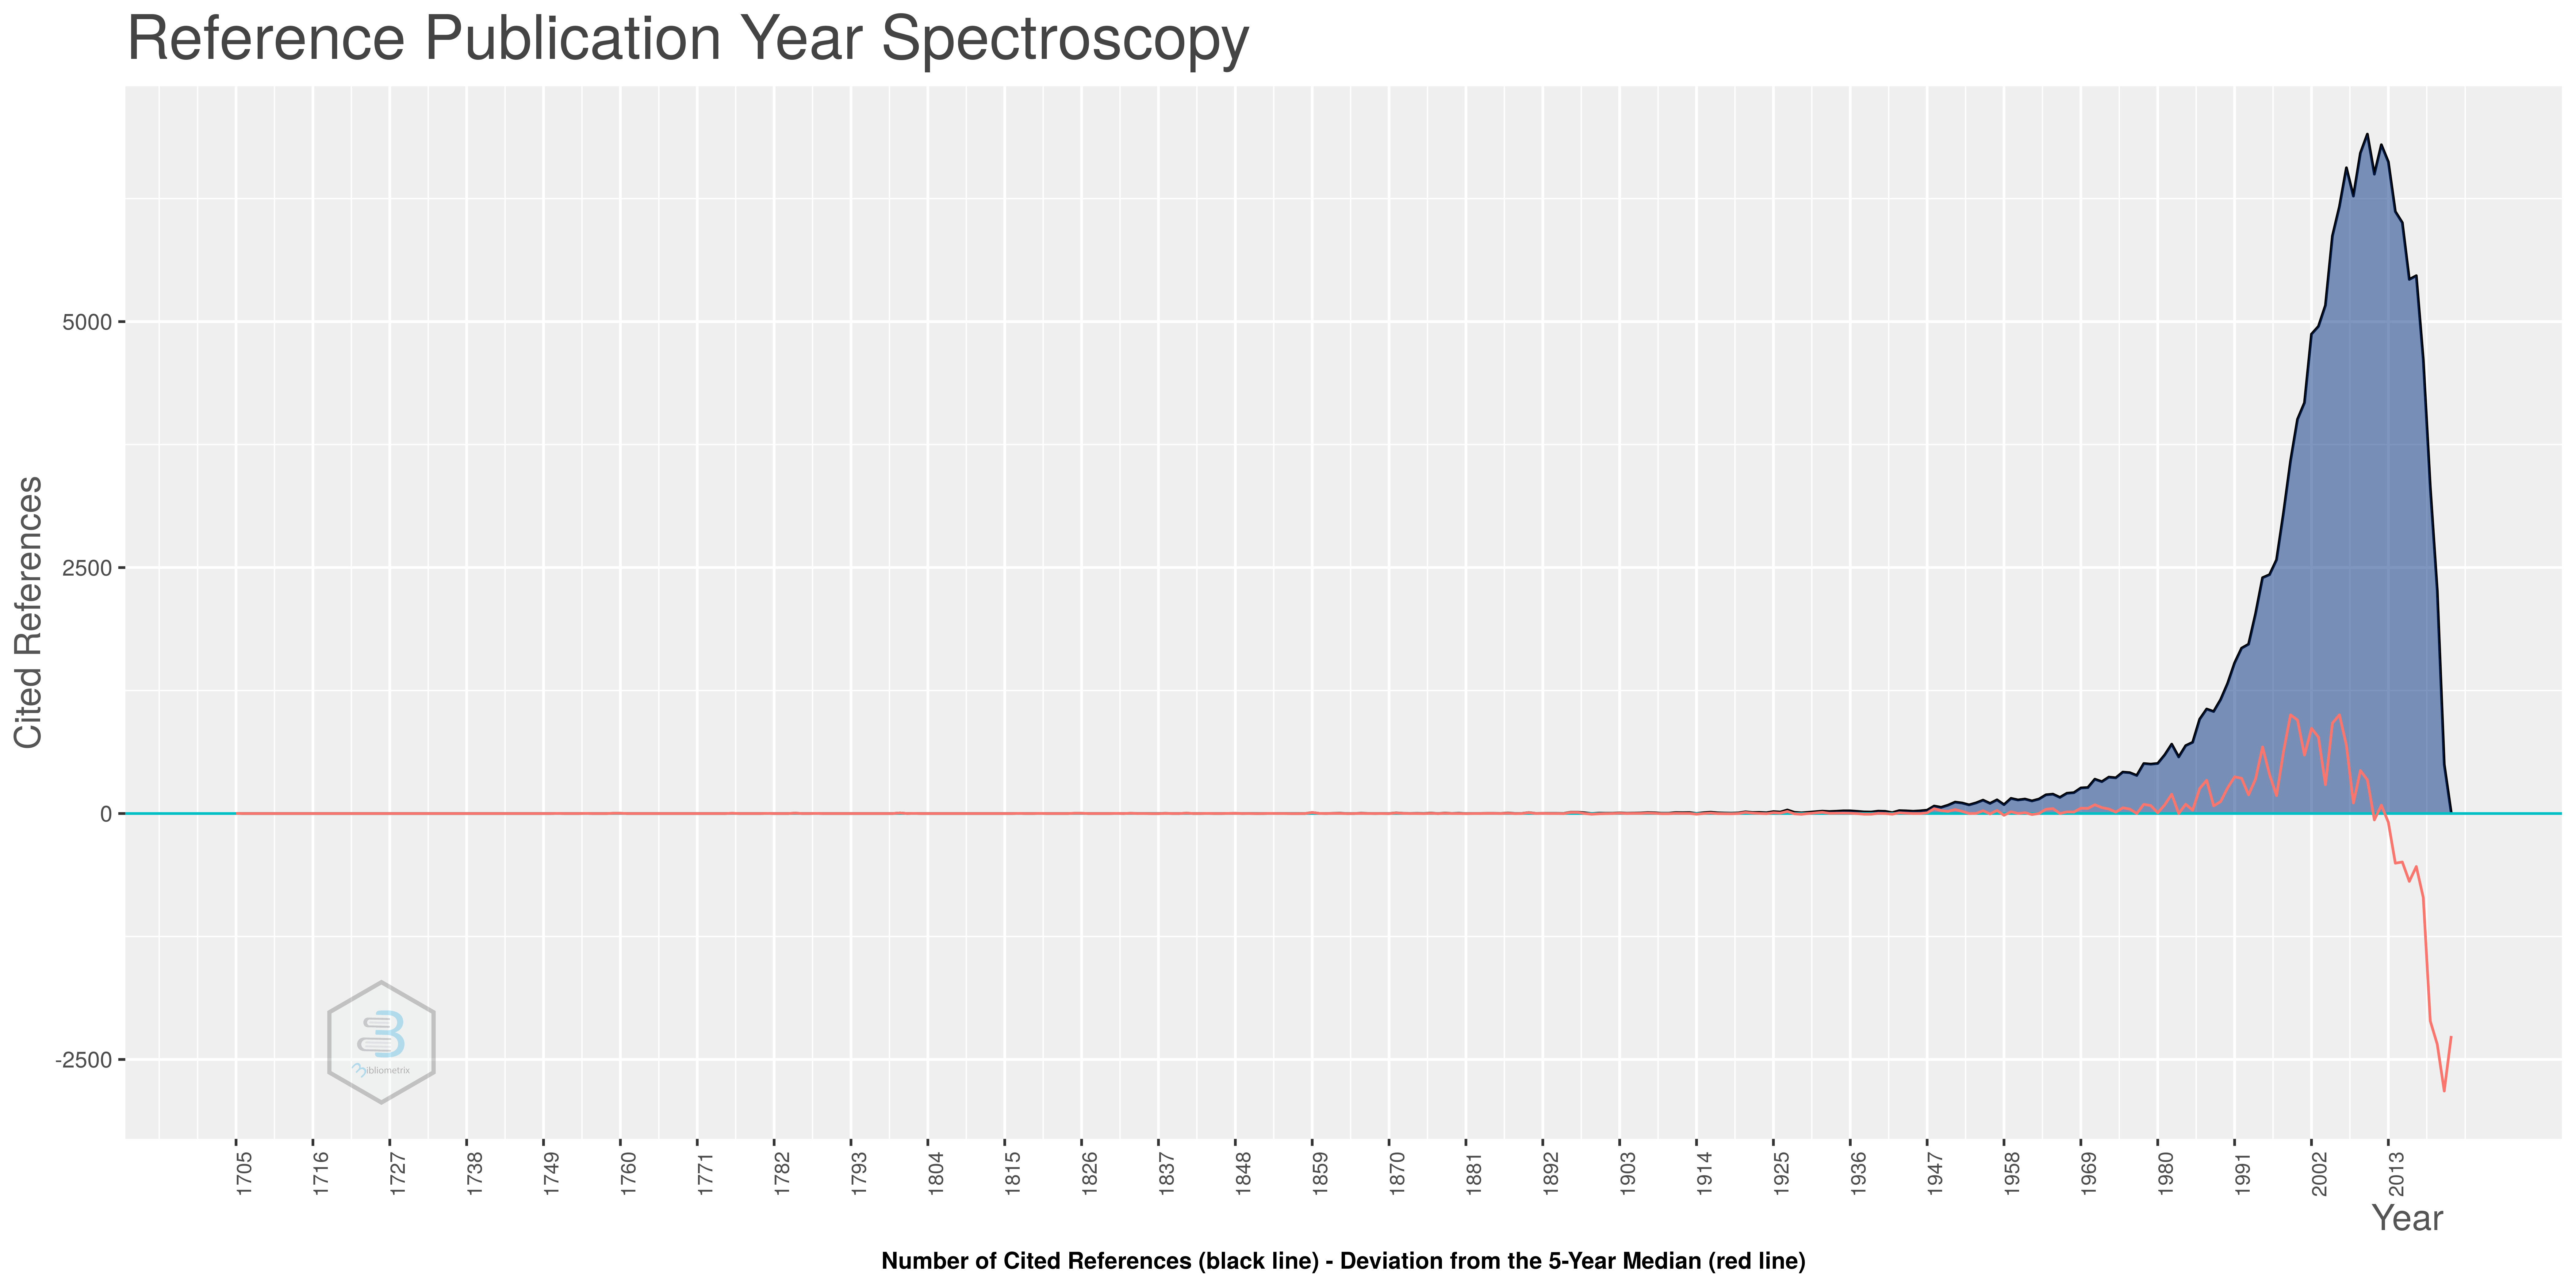
\includegraphics[width=1\textwidth]{experiments/jhcf/PesqBibliogr/SimulacaoMultiagente/WoS-20220203/Metricas/Documentos/MASSA2-ReferenceSpectroscopy.png}
    \caption{Espectroscopia (RPYS) completa das referências do \dataset\ MASSA2@jhcf.}
    \label{fig:MASSA2-ReferenceSpectroscopy}
\end{figure}

Se observamos a espectroscopia do mesmo \dataset\ apenas entre os anos de 1901 a 1970, como na figura \ref{fig:MASSA2-ReferenceSpectroscopy:1901:1970}, pode-se perceber um ponto de inflexão na curva, a partir do ano de 1946, que foi o período após o término da Segunda Guerra Mundial, quando o conhecimento científico que havia sido produzido sob sigilo no período da guerra começou a se disseminar pelo mundo.

\begin{figure}
    \centering
    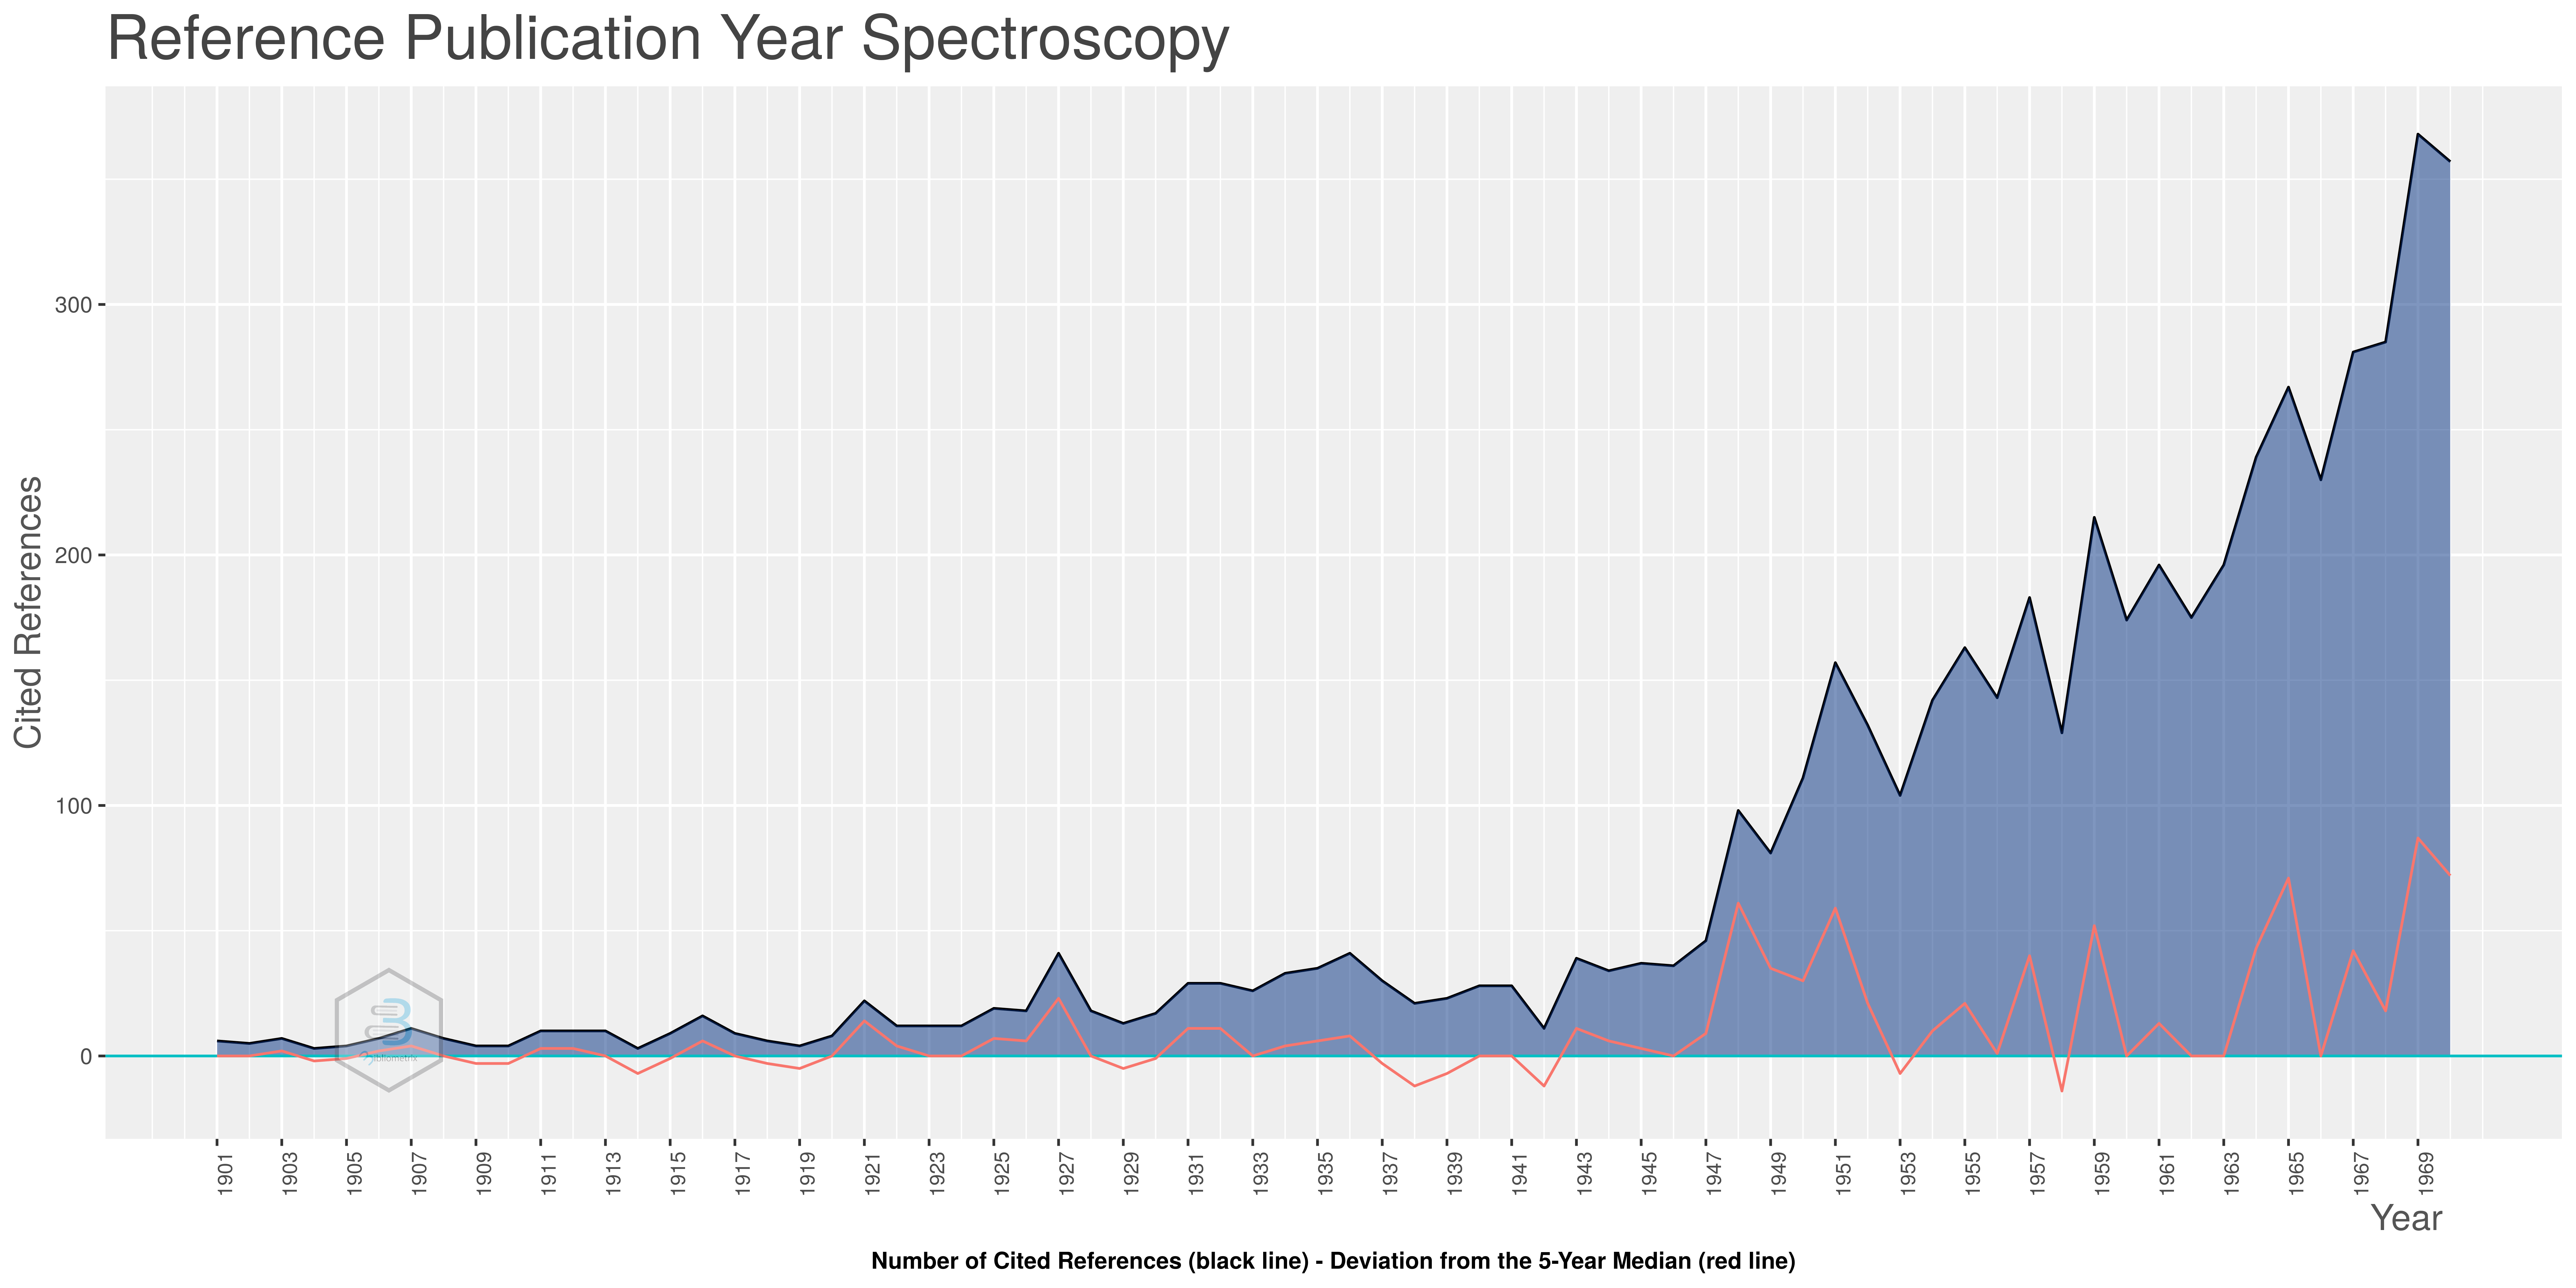
\includegraphics[width=1\textwidth]{experiments/jhcf/PesqBibliogr/SimulacaoMultiagente/WoS-20220203/Metricas/Documentos/MASSA2-ReferenceSpectroscopy-1901-1970.png}
    \caption{Espectroscopia (RPYS) das referências do \dataset\ MASSA2@jhcf, entre 1901 e 1970.}
    \label{fig:MASSA2-ReferenceSpectroscopy:1901:1970}
\end{figure}
    
Se observamos a espectroscopia do mesmo \dataset\ apenas entre os anos de 1971 a 2019, como na figura \ref{fig:MASSA2-ReferenceSpectroscopy:1971:2019}, pode-se perceber um ponto de declínio no volume de citações a partir do ano de 2010, sugerindo que esse campo de conhecimento atingiu sua maturidade cerca de 10 anos atrás.

\begin{figure}
    \centering
    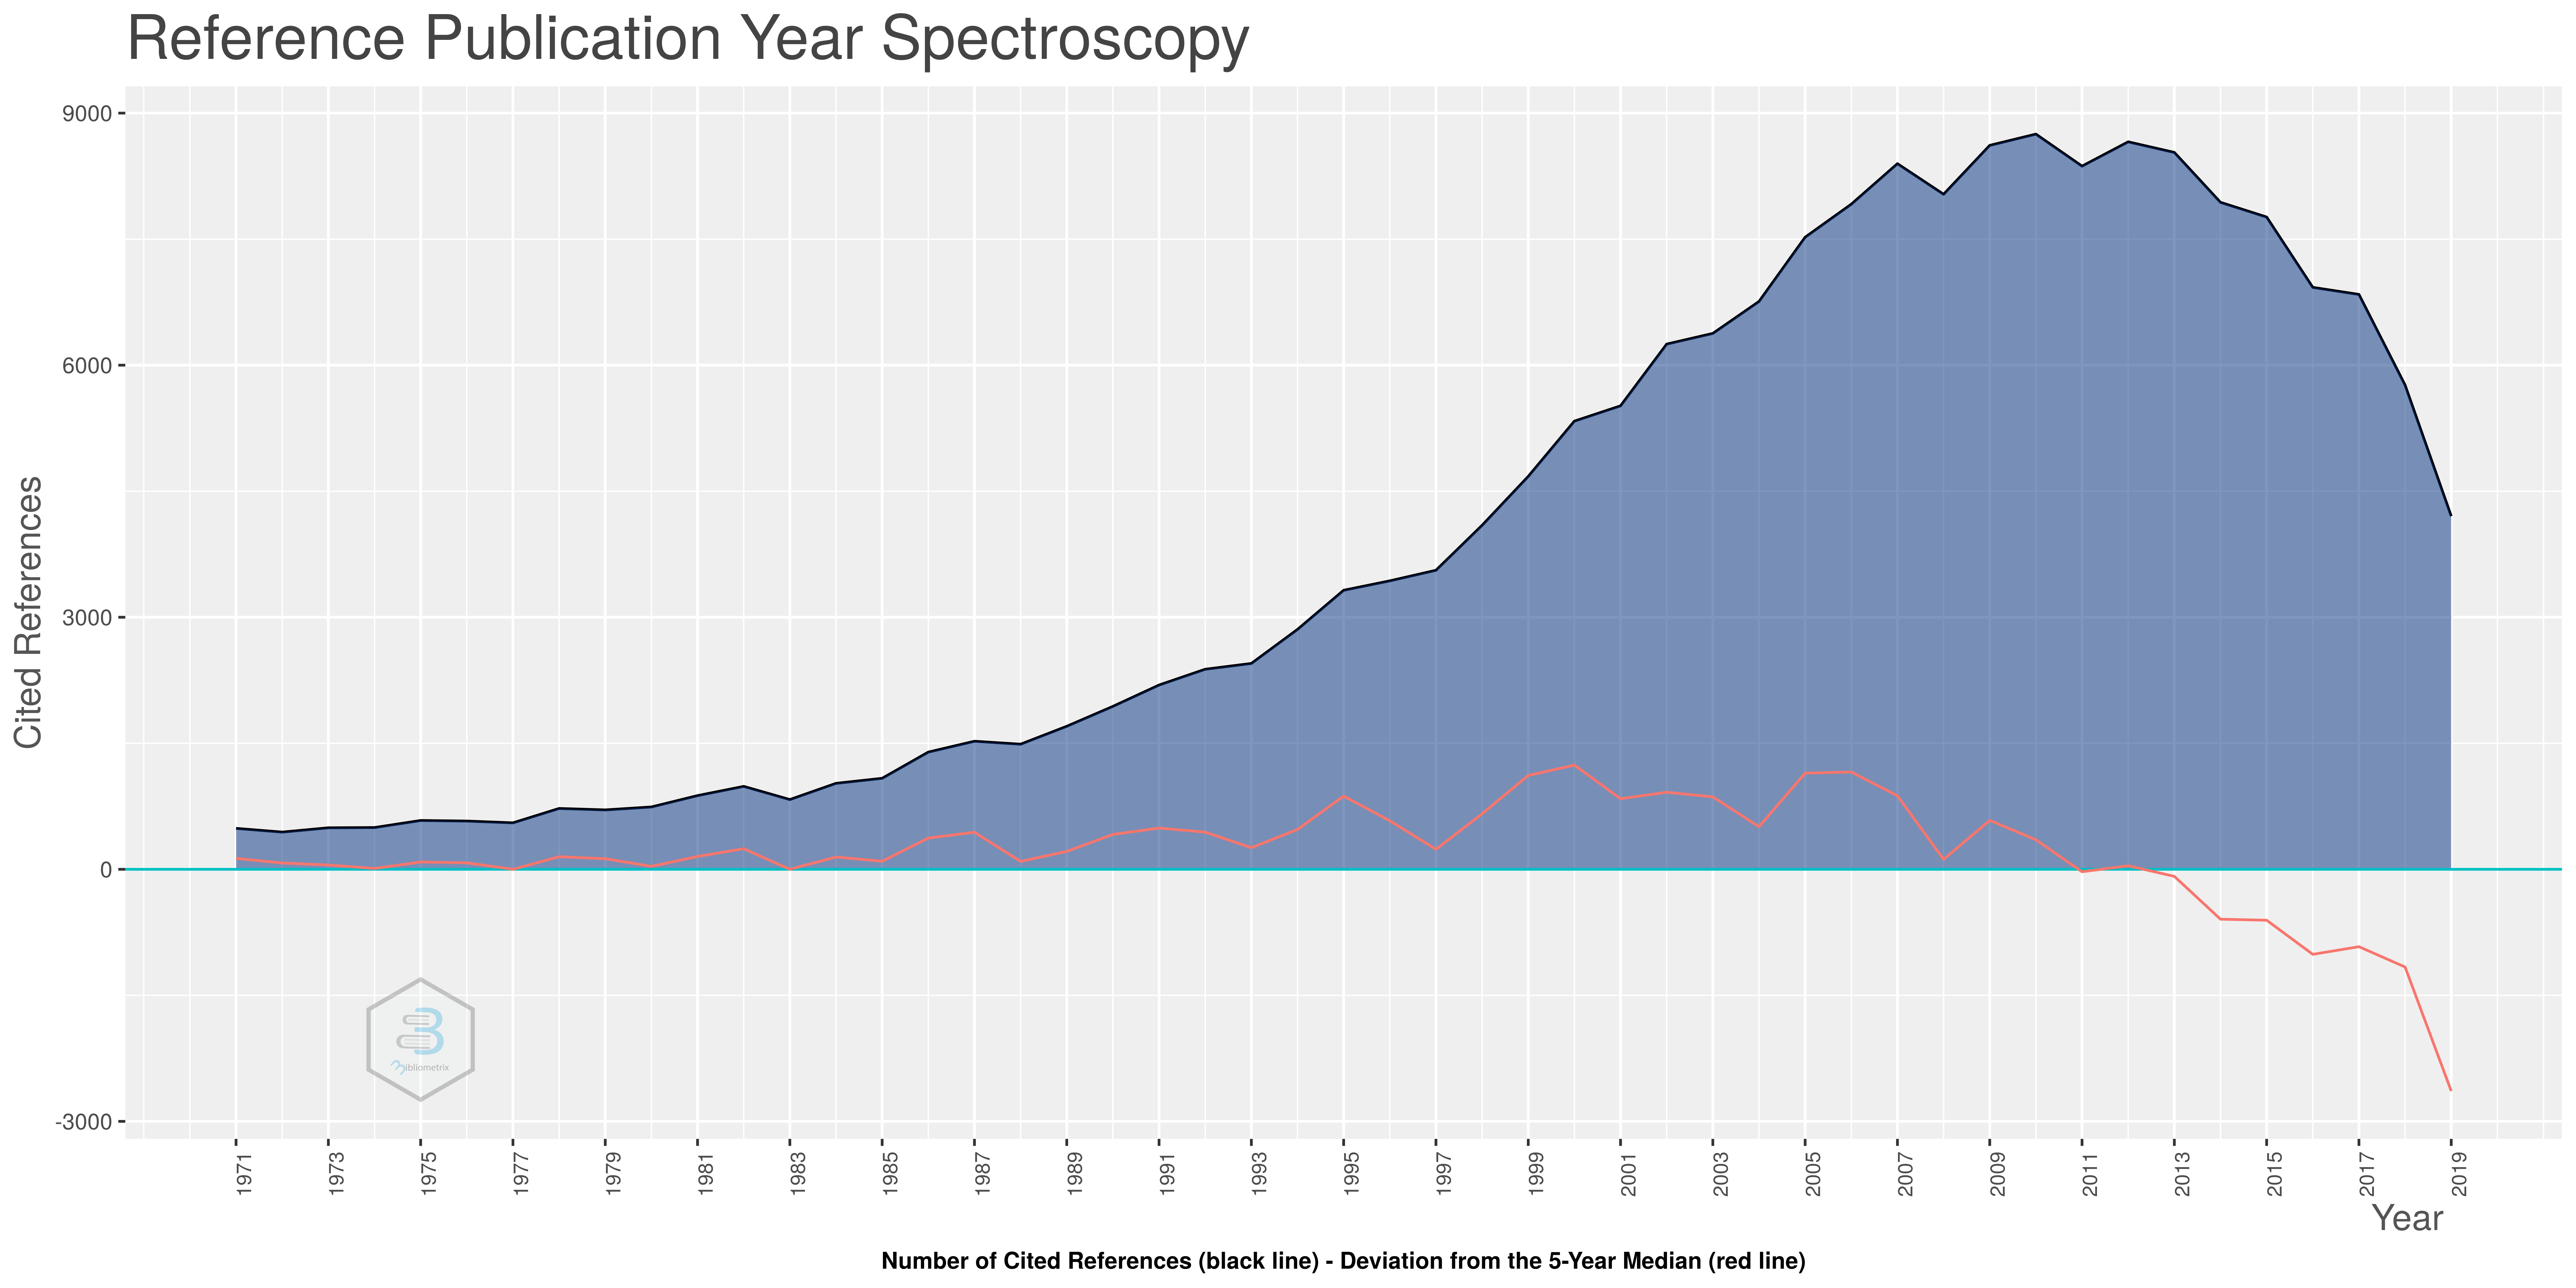
\includegraphics[width=1\textwidth]{experiments/jhcf/PesqBibliogr/SimulacaoMultiagente/WoS-20220203/Metricas/Documentos/MASSA2-ReferenceSpectroscopy-1971-2019.png}
    \caption{Espectroscopia (RPYS) das referências do \dataset\ MASSA2@jhcf, entre 1971 e 2019.}
    \label{fig:MASSA2-ReferenceSpectroscopy:1971:2019}
\end{figure}

\paragraph{Uso de palavras dentro dos artigos no \dataset}

As últimas das métricas aplicadas a documentos, disponíveis para aplicação no Bibliometrix é baseada na ocorrência de termos no texto dos documentos. A mais comum delas é baseada na simples contagem de frequência das palavras, como ilustra a tabela \ref{tab:MASSA2:Word:Occurrences}, com os 40 termos mais frequentes em uso.

\begin{table}[htp]
    \centering
\footnotesize
\csvreader[tabular = {|l|r|l|},
separator=semicolon,
filter={\value{csvrow}<40}
%,filter not strcmp={\csvcolii}{},
, table head = \hline\hline \# & Palavra (termo) & Frequência \\ \hline\hline,
table foot = \hline\hline
]{experiments/jhcf/PesqBibliogr/SimulacaoMultiagente/WoS-20220203/Metricas/Documentos/MASSA2-Most_Frequent_Words.csv}{Words=\palavra, Occurrences=\freq}{ \thecsvrow & \palavra & \freq}

    \caption{40 palavras (termos) mais frequentes no \dataset\ MASSA2@jhcf.}
    \label{tab:MASSA2:Word:Occurrences}
\end{table}

Outras formas de apresentação alternativas são apresentadas nas duas figuras a seguir, que ilustram de forma diferente a mesma informação, como em:
\begin{description}
    \item [Word Cloud] Uma nuvem de palavras, na figura \ref{fig:MASSA2-WordCloud-100words}, com evidencias para as 100 palavras mais frequentes;
    \item [Tree Map] Um mapa em árvore, na figura \ref{fig:MASSA2-TreeMap}, com evidências para as 50 palavras mais frequentes;
\end{description}

\begin{figure}
    \centering
    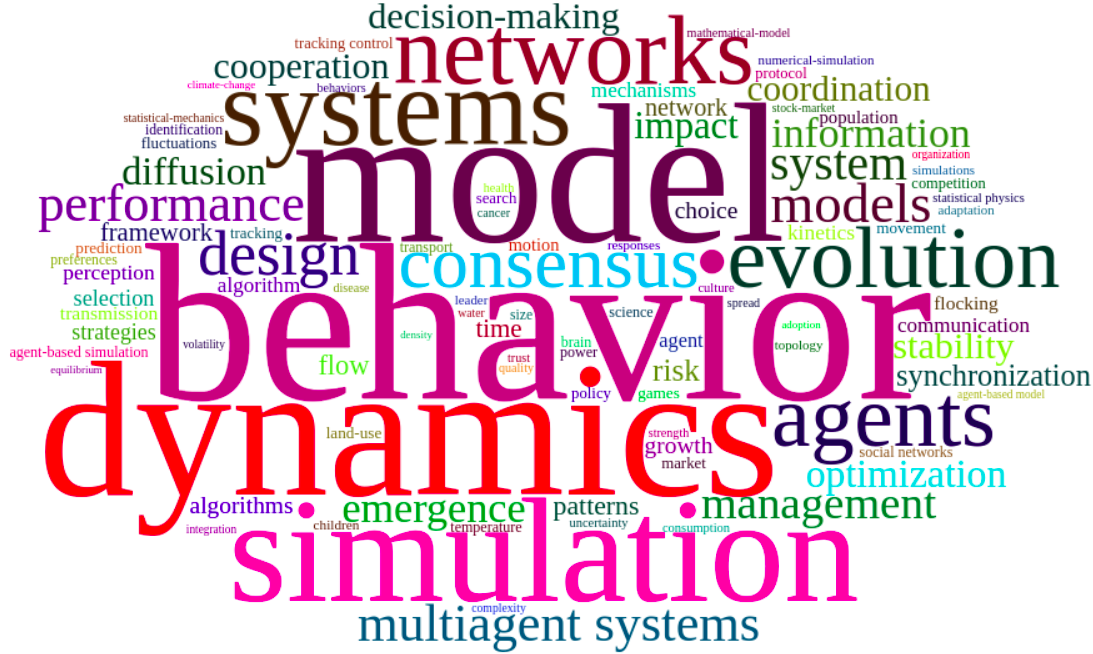
\includegraphics[width=1\textwidth]{experiments/jhcf/PesqBibliogr/SimulacaoMultiagente/WoS-20220203/Metricas/Documentos/MASSA2-WordCloud-100words.png}
    \caption{Nuvem dos 100 termos mais frequentes do \dataset\ MASSA2@jhcf.}
    \label{fig:MASSA2-WordCloud-100words}
\end{figure}

\begin{figure}
    \centering
    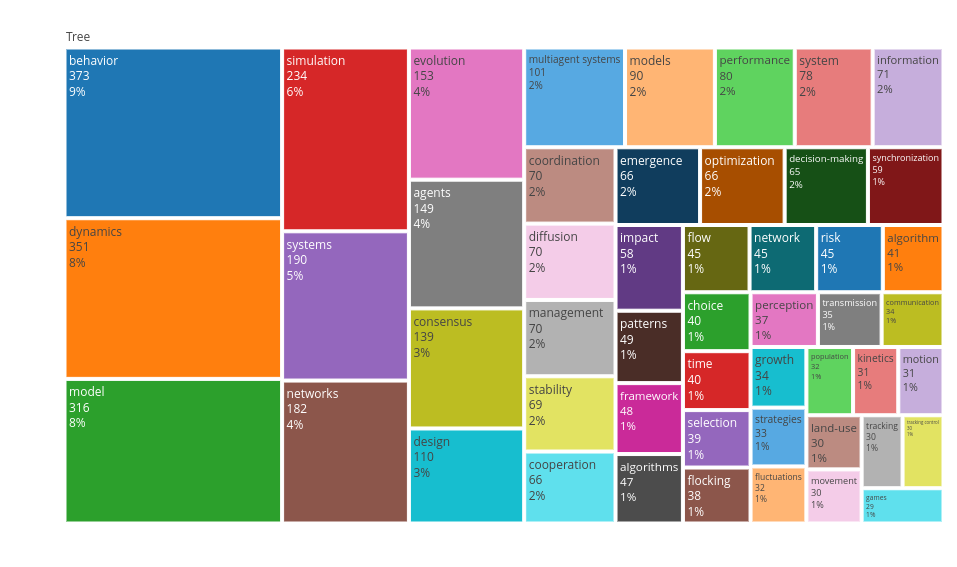
\includegraphics[width=1\textwidth]{experiments/jhcf/PesqBibliogr/SimulacaoMultiagente/WoS-20220203/Metricas/Documentos/MASSA2-TreeMap.png}
    \caption{\textit{Tree Map} dos 50 termos mais frequentes do \dataset\ MASSA2@jhcf.}
    \label{fig:MASSA2-TreeMap}
\end{figure}

Por fim, o Bibliometrix permite apresentar o uso dos termos ordenado temporalmente, como nas duas figuras a seguir:
\begin{description}
    \item [Word Growth / Word Dynamics] que mostra o crescimento de uso das palavras mais frequentes, como na figura \ref{fig:MASSA2-WordDynamics};
    \item [Trending topics] que mostra as tendências para uso de determinadas palavras em determinadas faixas de tempo, como em \ref{fig:MASSA2-TrendTopics}. Para obtenção do gráfico foram determinados os seguintes valores para os parâmetros: frequência mínima de ocorrência para que um termo seja considerado = 15, quantidade máxima de tópicos por ano = 7.
\end{description}

\begin{figure}
    \centering
    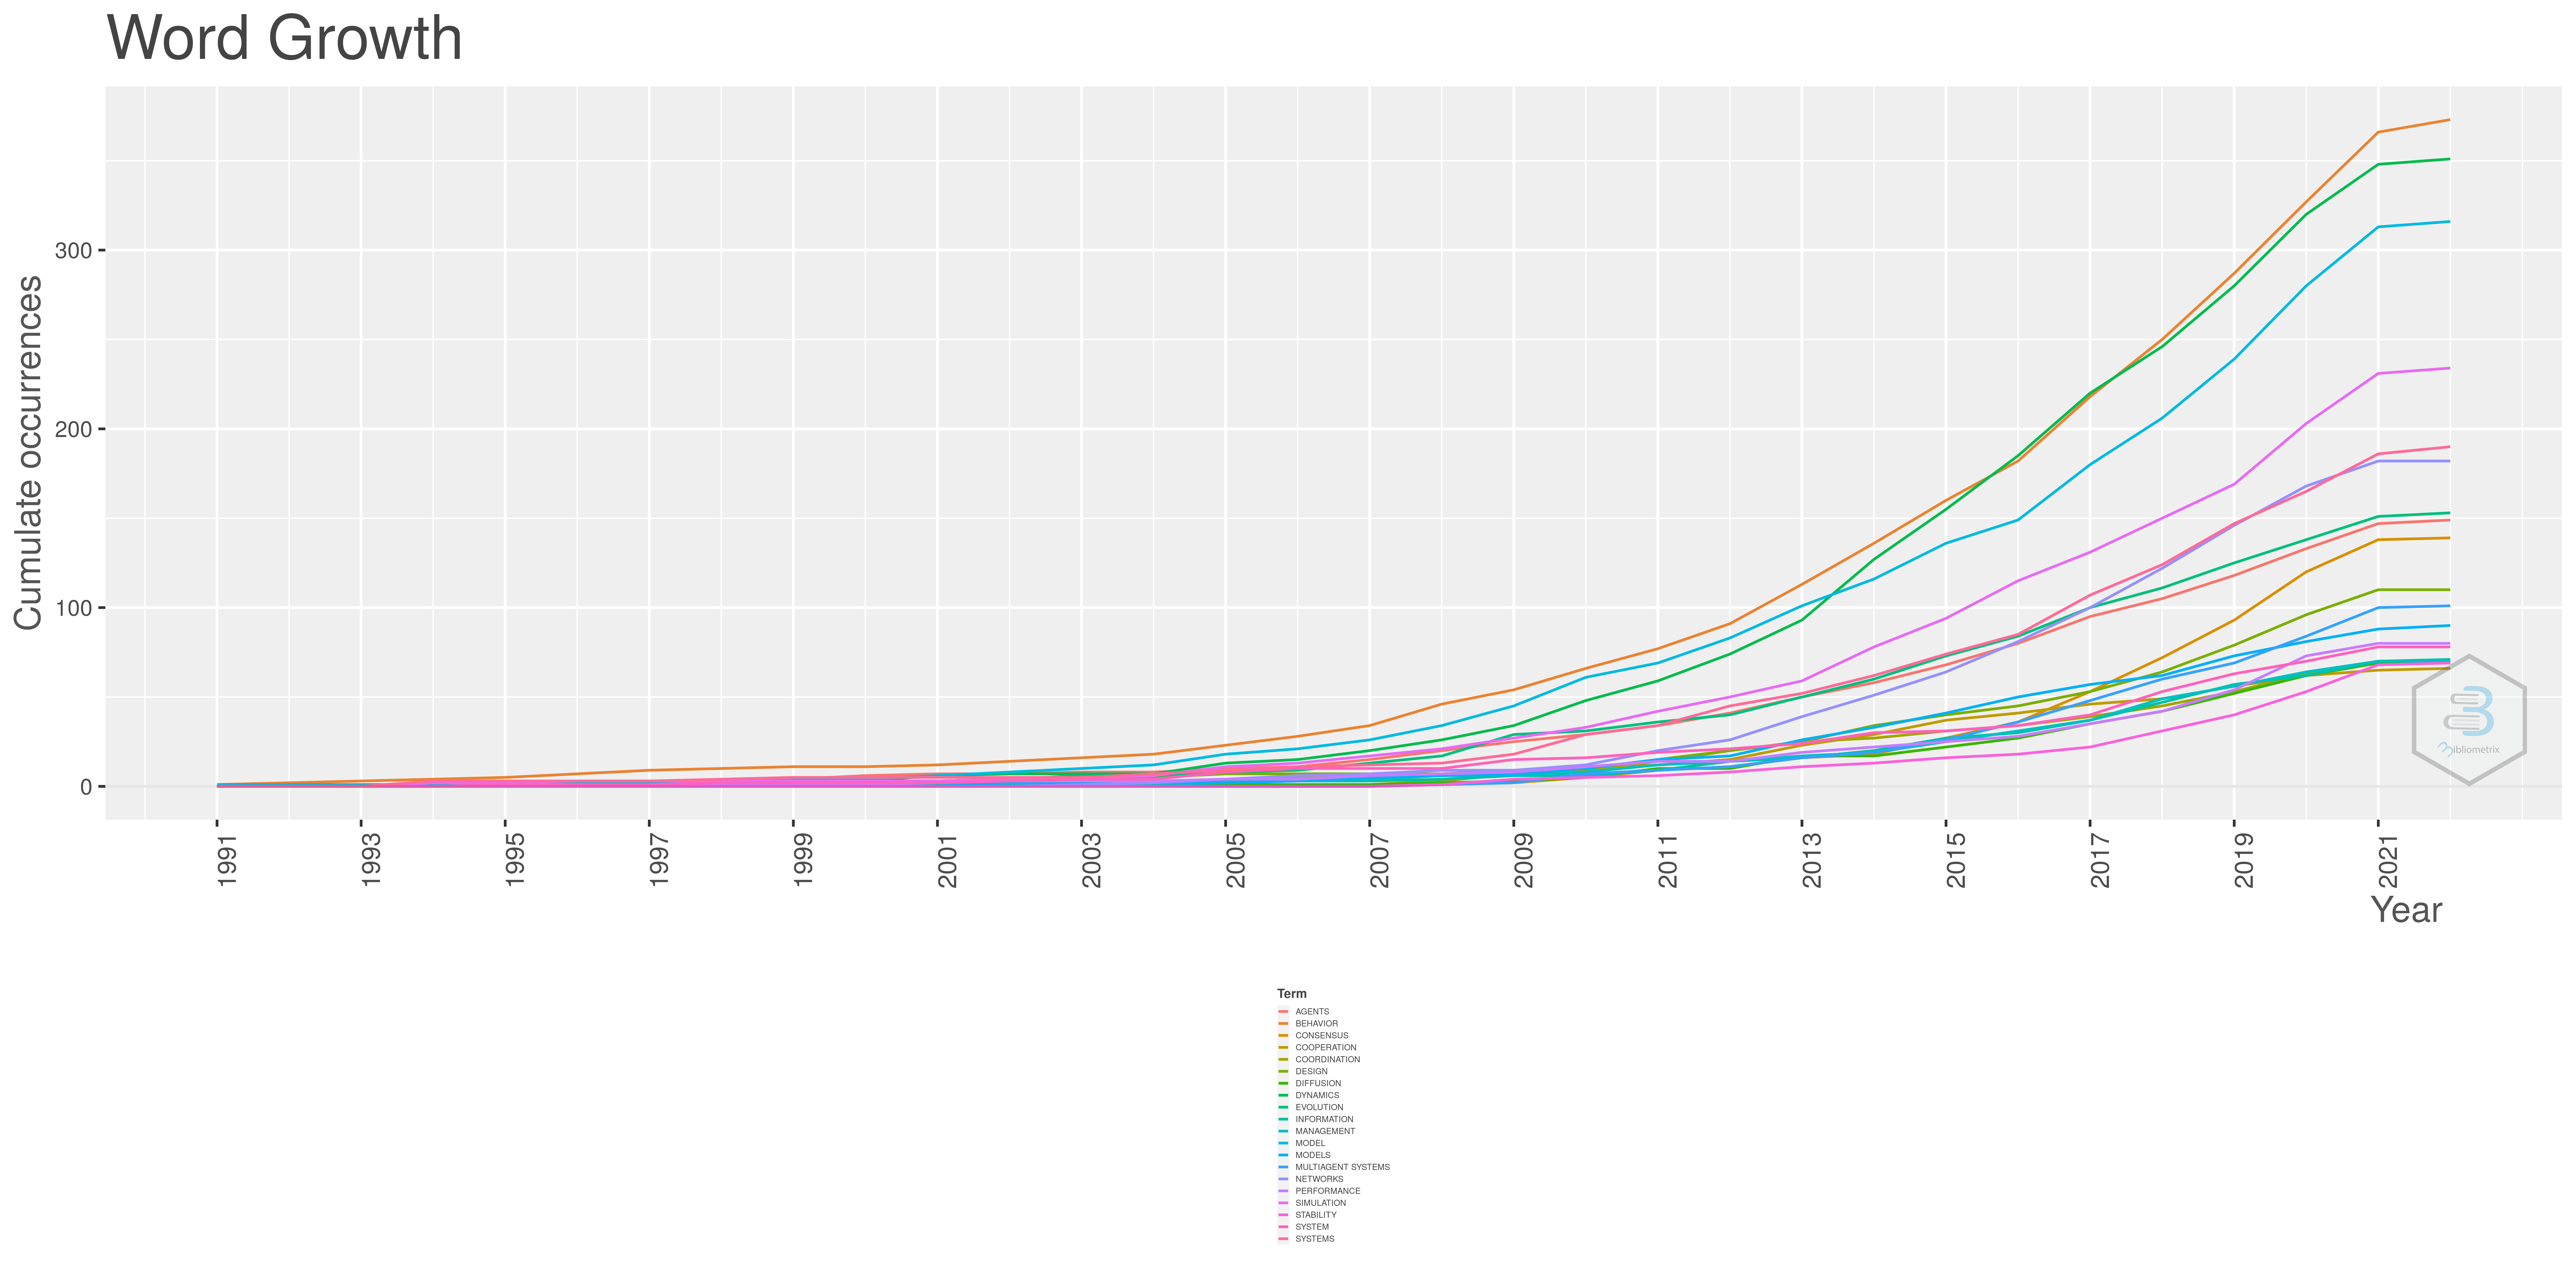
\includegraphics[width=1\textwidth]{experiments/jhcf/PesqBibliogr/SimulacaoMultiagente/WoS-20220203/Metricas/Documentos/MASSA2-WordDynamics.png}
    \caption{Dinâmica de uso ao longo do tempo, dos 20 termos mais frequentes do \dataset\ MASSA2@jhcf.}
    \label{fig:MASSA2-WordDynamics}
\end{figure}

\begin{figure}
    \centering
    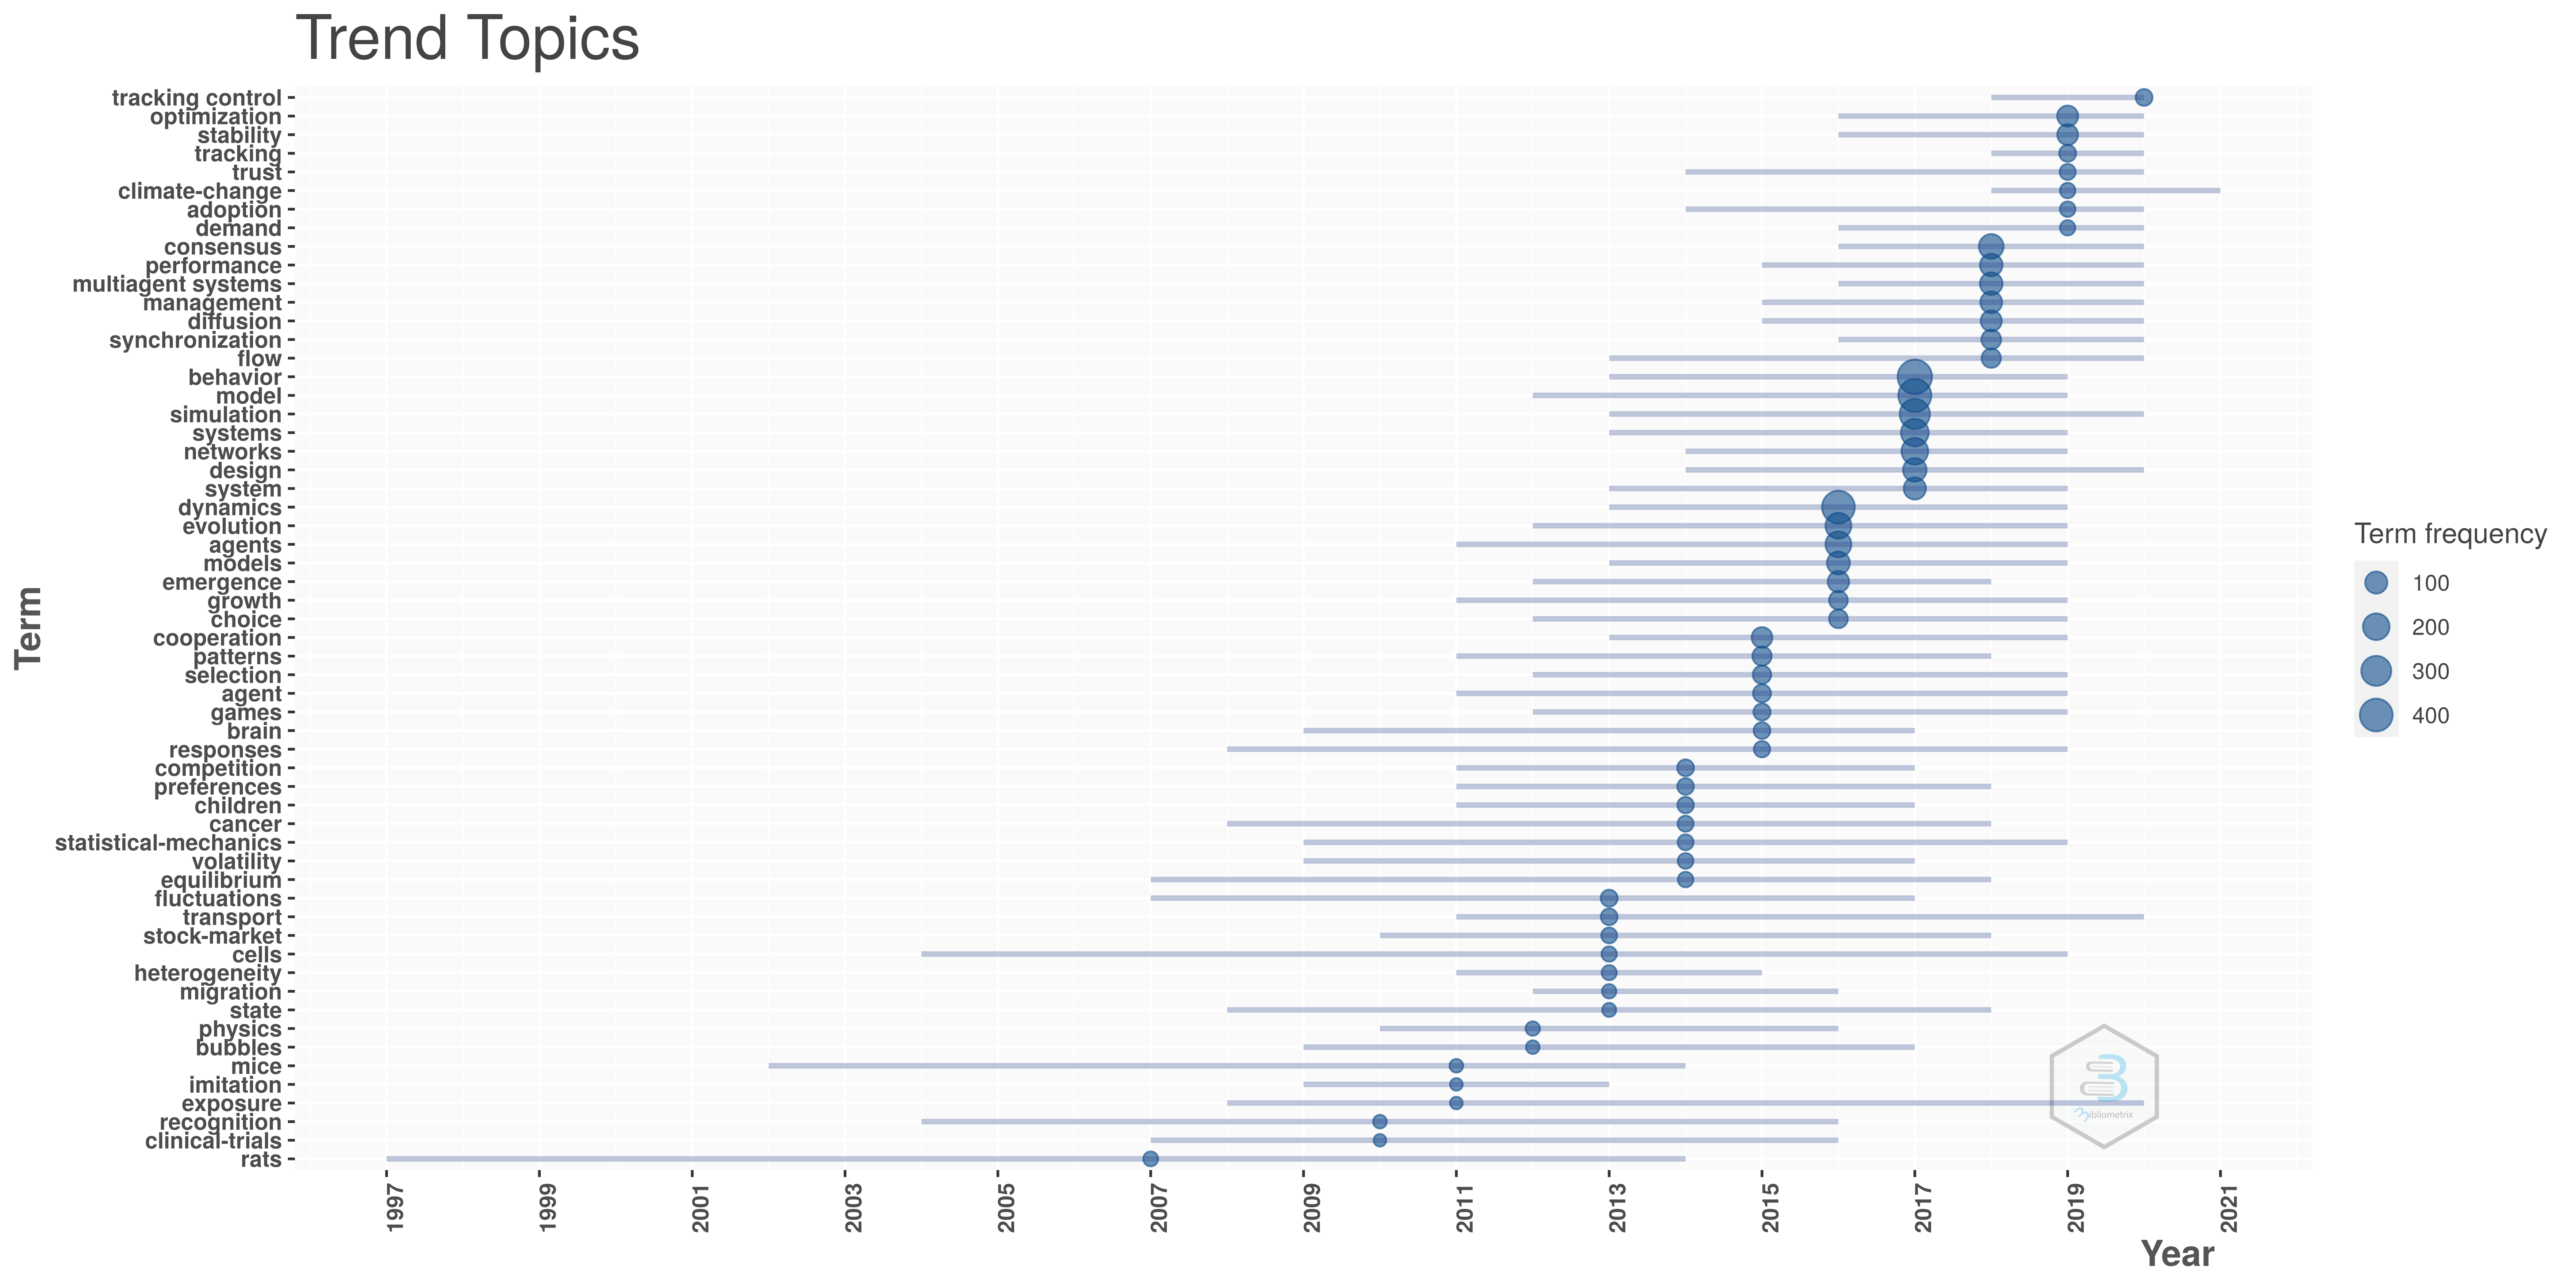
\includegraphics[angle=90,width=1\textwidth,height=0.93\textheight]{experiments/jhcf/PesqBibliogr/SimulacaoMultiagente/WoS-20220203/Metricas/Documentos/MASSA2-TrendTopics-WF=15:WPY=7.png}
    \caption{\textit{Trending Topics} do \dataset\ MASSA2@jhcf, WF = 15, WPY=7.}
    \label{fig:MASSA2-TrendTopics}
\end{figure}

\subsection{Métricas para Autores}

Um autor escreve um documento científico, que eventualmente é publicado. Ao escrever esse documento cita outros, e eventualmente o trabalho do autor também é citado. Se é citado, é porque é relevante, e daí infere-se que teve impacto. Com base na medica bruta da citação, várias métricas podem ser criadas. Algumas delas são aplicadas a seguir. 

\subsubsection{Autores mais produtivos no \dataset}

A tabela \ref{tab:MASSA2:Author:Production} apresenta a lista ordenada e decrescente dos autores com maior número de artigos no \dataset. A coluna mais à direita divide esse primeiro valor pelo número de autores nos artigos.

\begin{table}[htp]
    \centering
\footnotesize
\csvreader[tabular = {|r|l|r|r|},
filter={\value{csvrow}<40}
%,filter not strcmp={\csvcolii}{},
, table head = \hline\hline \# & Autor & Qtd. de artigos & Qtd. Proporcional \\ \hline\hline,
table foot = \hline\hline
]{experiments/jhcf/PesqBibliogr/SimulacaoMultiagente/WoS-20220203/Metricas/Authors/MASSA2-Most-Productive-Authors.csv}
{Authors=\autor,Articles=\qtdart,Fractionalized=\artfrac}{ \thecsvrow & \autor & \qtdart & \artfrac}
    \caption{20 autores com mais artigos no \dataset\ MASSA2@jhcf.}
    \label{tab:MASSA2:Author:Production}
\end{table}

\subsubsection{Autores mais relevantes localmente citados}

A tabela \ref{tab:MASSA2:Author:Production:Local} apresenta a lista ordenada e decrescente dos autores com maior número de artigos citados por outros artigos no \dataset. Esses são, possivelmente, os autores mais impactantes para o estado da arte no \dataset\ MASSA2@jhcf.

\begin{table}[htp]
    \centering
\footnotesize
\csvreader[tabular = {|r|l|r|},
filter={\value{csvrow}<40},
%,filter not strcmp={\csvcolii}{},
table head = \hline\hline \# & Autor & Qtd artigos\\ \hline\hline,
table foot = \hline\hline]
{experiments/jhcf/PesqBibliogr/SimulacaoMultiagente/WoS-20220203/Metricas/Authors/MASSA2-Most-Local-Cited-Authors.csv}
{Author=\autor,LocalCitations=\qtdcit}
{ \thecsvrow & \autor & \qtdcit}
\caption{20 autores com mais artigos citados por outros artigos no \dataset\ MASSA2@jhcf.}
    \label{tab:MASSA2:Author:Production:Local}
\end{table}

Uma busca na aba Filter, do Bibliometrix, permite explorar os artigos mais citados desses autores, alguns tem seus títulos listados a seguir:
\begin{description}
    \item [SCHWARZ N] 
    \begin{itemize}
        \item DESCRIBING HUMAN DECISIONS IN AGENT-BASED MODELS - ODD PLUS D, AN EXTENSION OF THE ODD PROTOCOL;
        \item AGENT-BASED MODELING OF THE DIFFUSION OF ENVIRONMENTAL INNOVATIONS - AN EMPIRICAL APPROACH;
    \end{itemize}
    \item [SU HS, WANG XF] 
    \begin{itemize}
        \item FLOCKING OF MULTI-AGENTS WITH A VIRTUAL LEADER;
        \item AGENT-BASED MODELING OF THE DIFFUSION OF ENVIRONMENTAL INNOVATIONS - AN EMPIRICAL APPROACH;
    \end{itemize}
    \item [LIAO XF] 
    \begin{itemize}
        \item EVENT-TRIGGERING SAMPLING BASED LEADER-FOLLOWING CONSENSUS IN SECOND-ORDER MULTI-AGENT SYSTEMS;
    \end{itemize}    
\end{description}

\subsubsection{Variação da produtividade dos autores ao longo do tempo}

Os cientistas são seres humanos, que também tem um ciclo de vida de iniciante, muito produtivo, menos produtivo, e não produtivo.
Diagramas como o da figura \ref{fig:MASSA2-TopAuthorsProductionOverTime} apresentam esse ciclo de vida, em relação ao \dataset\ MASSA2@jhcf.

\begin{figure}
    \centering
    
\includegraphics[angle=90,width=1\textwidth,height=0.93\textheight]{experiments/jhcf/PesqBibliogr/SimulacaoMultiagente/WoS-20220203/Metricas/Authors/MASSA2-TopAuthorsProductionOverTime.png}
    \caption{Variação da produção dos autores de maior impacto, do \dataset\ MASSA2@jhcf.}
    \label{fig:MASSA2-TopAuthorsProductionOverTime}
\end{figure}

\subsubsection{Lei de Lotka}

A Lei de Lotka (ver \url{https://en.wikipedia.org/wiki/Lotka\%27s_law}) estabelece uma distribuição de frequência aproximadamente inversamente quadrática ou cúbica, para o número de artigos publicados pelos autores de qualquer área do conhecimento. Isso é, se 1000 pessoas publicam ao longo de sua contribuição para o campo de conhecimento apenas um documento, então
entre $1000/x^{2}$ a $1000/x^{3}$ publicam $x$ documentos. Ou seja, entre
$1000/2^{2}$ a $1000/2^{3}$ pessoas publicam dois documentos, $1000/3^{2}$ a $1000/3^{3}$ pessoas publicam três documentos etc.

Se os dados empíricos do \dataset\ são alinhados à essas curvas, então supor dizer que o \dataset\ é bem formado. Será que isso ocorre com a tabela \ref{}, criada para o \dataset\ MASSA2@jhcf?

\begin{table}[htp]
    \centering
\footnotesize
\csvreader[
separator=semicolon,
tabular = {|r|l|r|r|r|},
filter={\value{csvrow}<40},
%,filter not strcmp={\csvcolii}{},
table head = \hline\hline \# & Qtd Autores & Qtd artigos & Lotka 2 & Lotka 3\\ \hline\hline,
table foot = \hline\hline]
{experiments/jhcf/PesqBibliogr/SimulacaoMultiagente/WoS-20220203/Metricas/Authors/MASSA2-Lotka_Law.csv}
{}
{ \thecsvrow & \csvcolii & \csvcoli & \csvcoliii & \csvcoliv}
\caption{Comparação do \dataset\ MASSA2@jhcf com a formulação geral da Lei de Lotka.}
    \label{tab:MASSA2:Author:Lotka}
\end{table}

\subsubsection{Medidas de Impacto dos Autores}

A partir da medida básica de citações (TC) podem ser criados vários índices, sendo os mais conhecidos os índices H (Ver \url{https://en.wikipedia.org/wiki/H-index}), G (Ver \url{https://en.wikipedia.org/wiki/G-index})e M (ver \url{https://en.wikipedia.org/wiki/Author-level_metrics#m-index}).

As tabelas \ref{tab:MASSA2:Author:Impacto:H}, \ref{tab:MASSA2:Author:Impacto:G}, \ref{tab:MASSA2:Author:Impacto:M} e \ref{tab:MASSA2:Author:Impacto:Qtd:Publicacoes} mostram os autores mais proeminentes do \dataset\ ordenados com base em um desses índices ou com o simples volume total de publicação, em comparação aos demais índices.

Além dos índices e da quantidade total de citações (coluna TC), apresenta-se o volume de publicações (NP) e o ano de primeira publicação do autor (PY Start).

Observe que os índices H e G tendem a valorizar os autores mais estabilizados, enquanto que o índice M mostra os autores mais recentes, que tem menos anos de publicação.

Observe, adicionalmente, que a base para cálculo desses índices é o número total de citações, que tem alcance global, enquanto que o número de artigos publicados é o valor local.

\begin{table}[htp]
    \centering
\footnotesize
\csvreader[
separator=semicolon,
tabular = {|r|l|r|r|r|r|r|r|},
filter={\value{csvrow}<40},
%,filter not strcmp={\csvcolii}{},
table head = \hline\hline \# & Autor & Índice H & Índice G & Índice M & TC & NP & PY Start\\ \hline\hline,
table foot = \hline\hline]
{experiments/jhcf/PesqBibliogr/SimulacaoMultiagente/WoS-20220203/Metricas/Authors/MASSA2-H-Index-Author-Impact.csv}
{}
{ \thecsvrow & \csvcoli & \csvcolii & \csvcoliii & \csvcoliv & \csvcolv & \csvcolvi & \csvcolvii}
\caption{10 autores de maior impacto no \dataset\ MASSA2@jhcf, conforme o índice H.}
    \label{tab:MASSA2:Author:Impacto:H}
\end{table}

\begin{table}[htp]
    \centering
\footnotesize
\csvreader[
separator=semicolon,
tabular = {|r|l|r|r|r|r|r|r|},
filter={\value{csvrow}<40},
%,filter not strcmp={\csvcolii}{},
table head = \hline\hline \# & Autor & Índice H & Índice G & Índice M & TC & NP & PY Start\\ \hline\hline,
table foot = \hline\hline]
{experiments/jhcf/PesqBibliogr/SimulacaoMultiagente/WoS-20220203/Metricas/Authors/MASSA2-G-Index-Author-Impact.csv}
{}
{ \thecsvrow & \csvcoli & \csvcolii & \csvcoliii & \csvcoliv & \csvcolv & \csvcolvi & \csvcolvii}
\caption{10 autores de maior impacto no \dataset\ MASSA2@jhcf, conforme o índice G.}
    \label{tab:MASSA2:Author:Impacto:G}
\end{table}

\begin{table}[htp]
    \centering
\footnotesize
\csvreader[
separator=semicolon,
tabular = {|r|l|r|r|r|r|r|r|},
filter={\value{csvrow}<40},
%,filter not strcmp={\csvcolii}{},
table head = \hline\hline \# & Autor & Índice H & Índice G & Índice M & TC & NP & PY Start\\ \hline\hline,
table foot = \hline\hline]
{experiments/jhcf/PesqBibliogr/SimulacaoMultiagente/WoS-20220203/Metricas/Authors/MASSA2-M-Index-Author-Impact.csv}
{}
{ \thecsvrow & \csvcoli & \csvcolii & \csvcoliii & \csvcoliv & \csvcolv & \csvcolvi & \csvcolvii}
\caption{25 autores de maior impacto no \dataset\ MASSA2@jhcf, conforme o índice M.}
    \label{tab:MASSA2:Author:Impacto:M}
\end{table}

\begin{table}[htp]
    \centering
\footnotesize
\csvreader[
separator=semicolon,
tabular = {|r|l|r|r|r|r|r|r|},
filter={\value{csvrow}<40},
%,filter not strcmp={\csvcolii}{},
table head = \hline\hline \# & Autor & Índice H & Índice G & Índice M & TC & NP & PY Start\\ \hline\hline,
table foot = \hline\hline]
{experiments/jhcf/PesqBibliogr/SimulacaoMultiagente/WoS-20220203/Metricas/Authors/MASSA2-Total-Citations-Author-Impact.csv}
{}
{ \thecsvrow & \csvcoli & \csvcolii & \csvcoliii & \csvcoliv & \csvcolv & \csvcolvi & \csvcolvii}
\caption{25 autores de maior impacto no \dataset\ MASSA2@jhcf, conforme a quantidade de vezes que seus artigos foram globalmente citados.}
    \label{tab:MASSA2:Author:Impacto:Qtd:Publicacoes}
\end{table}

\subsubsection{Filiações dos autores às instituições de P\&D}

Os autores de documentos científicos são filiados como estudantes ou empregados em universidades e centros de pesquisa, e quando os publicam colocam o nome de suas filiações, criando a possibilidade de produção de \textit{rankings} para essas instituições. A tabela \ref{tab:MASSA2-Most-Relevant-Affiliations} apresenta as 40 instituições com maior produtividade, conforme o volume de artigos publicados presentes no \dataset. Ou seja, é nas instituições listadas na tabela onde possivelmente está mais avançado o conhecimento nesse tema. 

\begin{table}[htp]
    \centering
\footnotesize
\csvreader[
separator=comma,
tabular = {|r|l|r|},
filter={\value{csvrow}<40},
%,filter not strcmp={\csvcolii}{},
table head = \hline\hline \# & Instituição de filiação & Qtd de artigos publicados\\ \hline\hline,
table foot = \hline\hline]
{experiments/jhcf/PesqBibliogr/SimulacaoMultiagente/WoS-20220203/Metricas/Authors/MASSA2-Most-Relevant-Affiliations.csv}
{}
{ \thecsvrow & \csvcoli & \csvcolii }
\caption{40 Instituições mais produtivas no tema do \dataset\ MASSA2@jhcf, conforme a quantidade de artigos publicados por pessoas a elas filiadas.}
    \label{tab:MASSA2-Most-Relevant-Affiliations}
\end{table}

\subsubsection{Filiações dos autores aos Países}

As instituições às quais são filiados os autores são sediadas em países, o que permite estimar a produtividade e (ou) impacto dos países em um tema de conhecimento específico, como ilustra a tabela \ref{MASSA2-Most-Cited-Countries}, que mostra a quantidade de citações obtidas pelos artigos das instituições sediadas nesses países.

\begin{table}[htp]
    \centering
\footnotesize
\csvreader[
separator=semicolon,
tabular = {|r|l|r|r|},
filter={\value{csvrow}<40},
%,filter not strcmp={\csvcolii}{},
table head = \hline\hline \# & País de Filiação & Qtd. Citações & Média de Citação por Artigo\\ \hline\hline,
table foot = \hline\hline]
{experiments/jhcf/PesqBibliogr/SimulacaoMultiagente/WoS-20220203/Metricas/Authors/MASSA2-Most-Cited-Countries.csv}
{}
{ \thecsvrow & \csvcoli & \csvcolii & \csvcoliii}
\caption{40 países com maior impacto de citações no tema do \dataset\ MASSA2@jhcf.}
    \label{tab:MASSA2-Most-Cited-Countries}
\end{table}

\paragraph{Países dos autores principais dos artigos}

Cada artigo escrito por mais de um autor tem um autor responsável por receber as correspondências relativas ao artigo. Esse é o  \textit{corresponding author}. A figura \ref{fig:MASSA2-Corresponding-Authors-Country} apresenta, em ordem do maior para o menor volume de correspondentes por artigo, o volume publicado por cada país. SCP são as publicações cujos autores são todos do mesmo país. MCP envolve autores de mais de um país. Note que países como Japão, Índia e Irã, no \dataset\ em pauta, não parecem colaborar muito, de forma internacional.

\begin{figure}
    \centering
    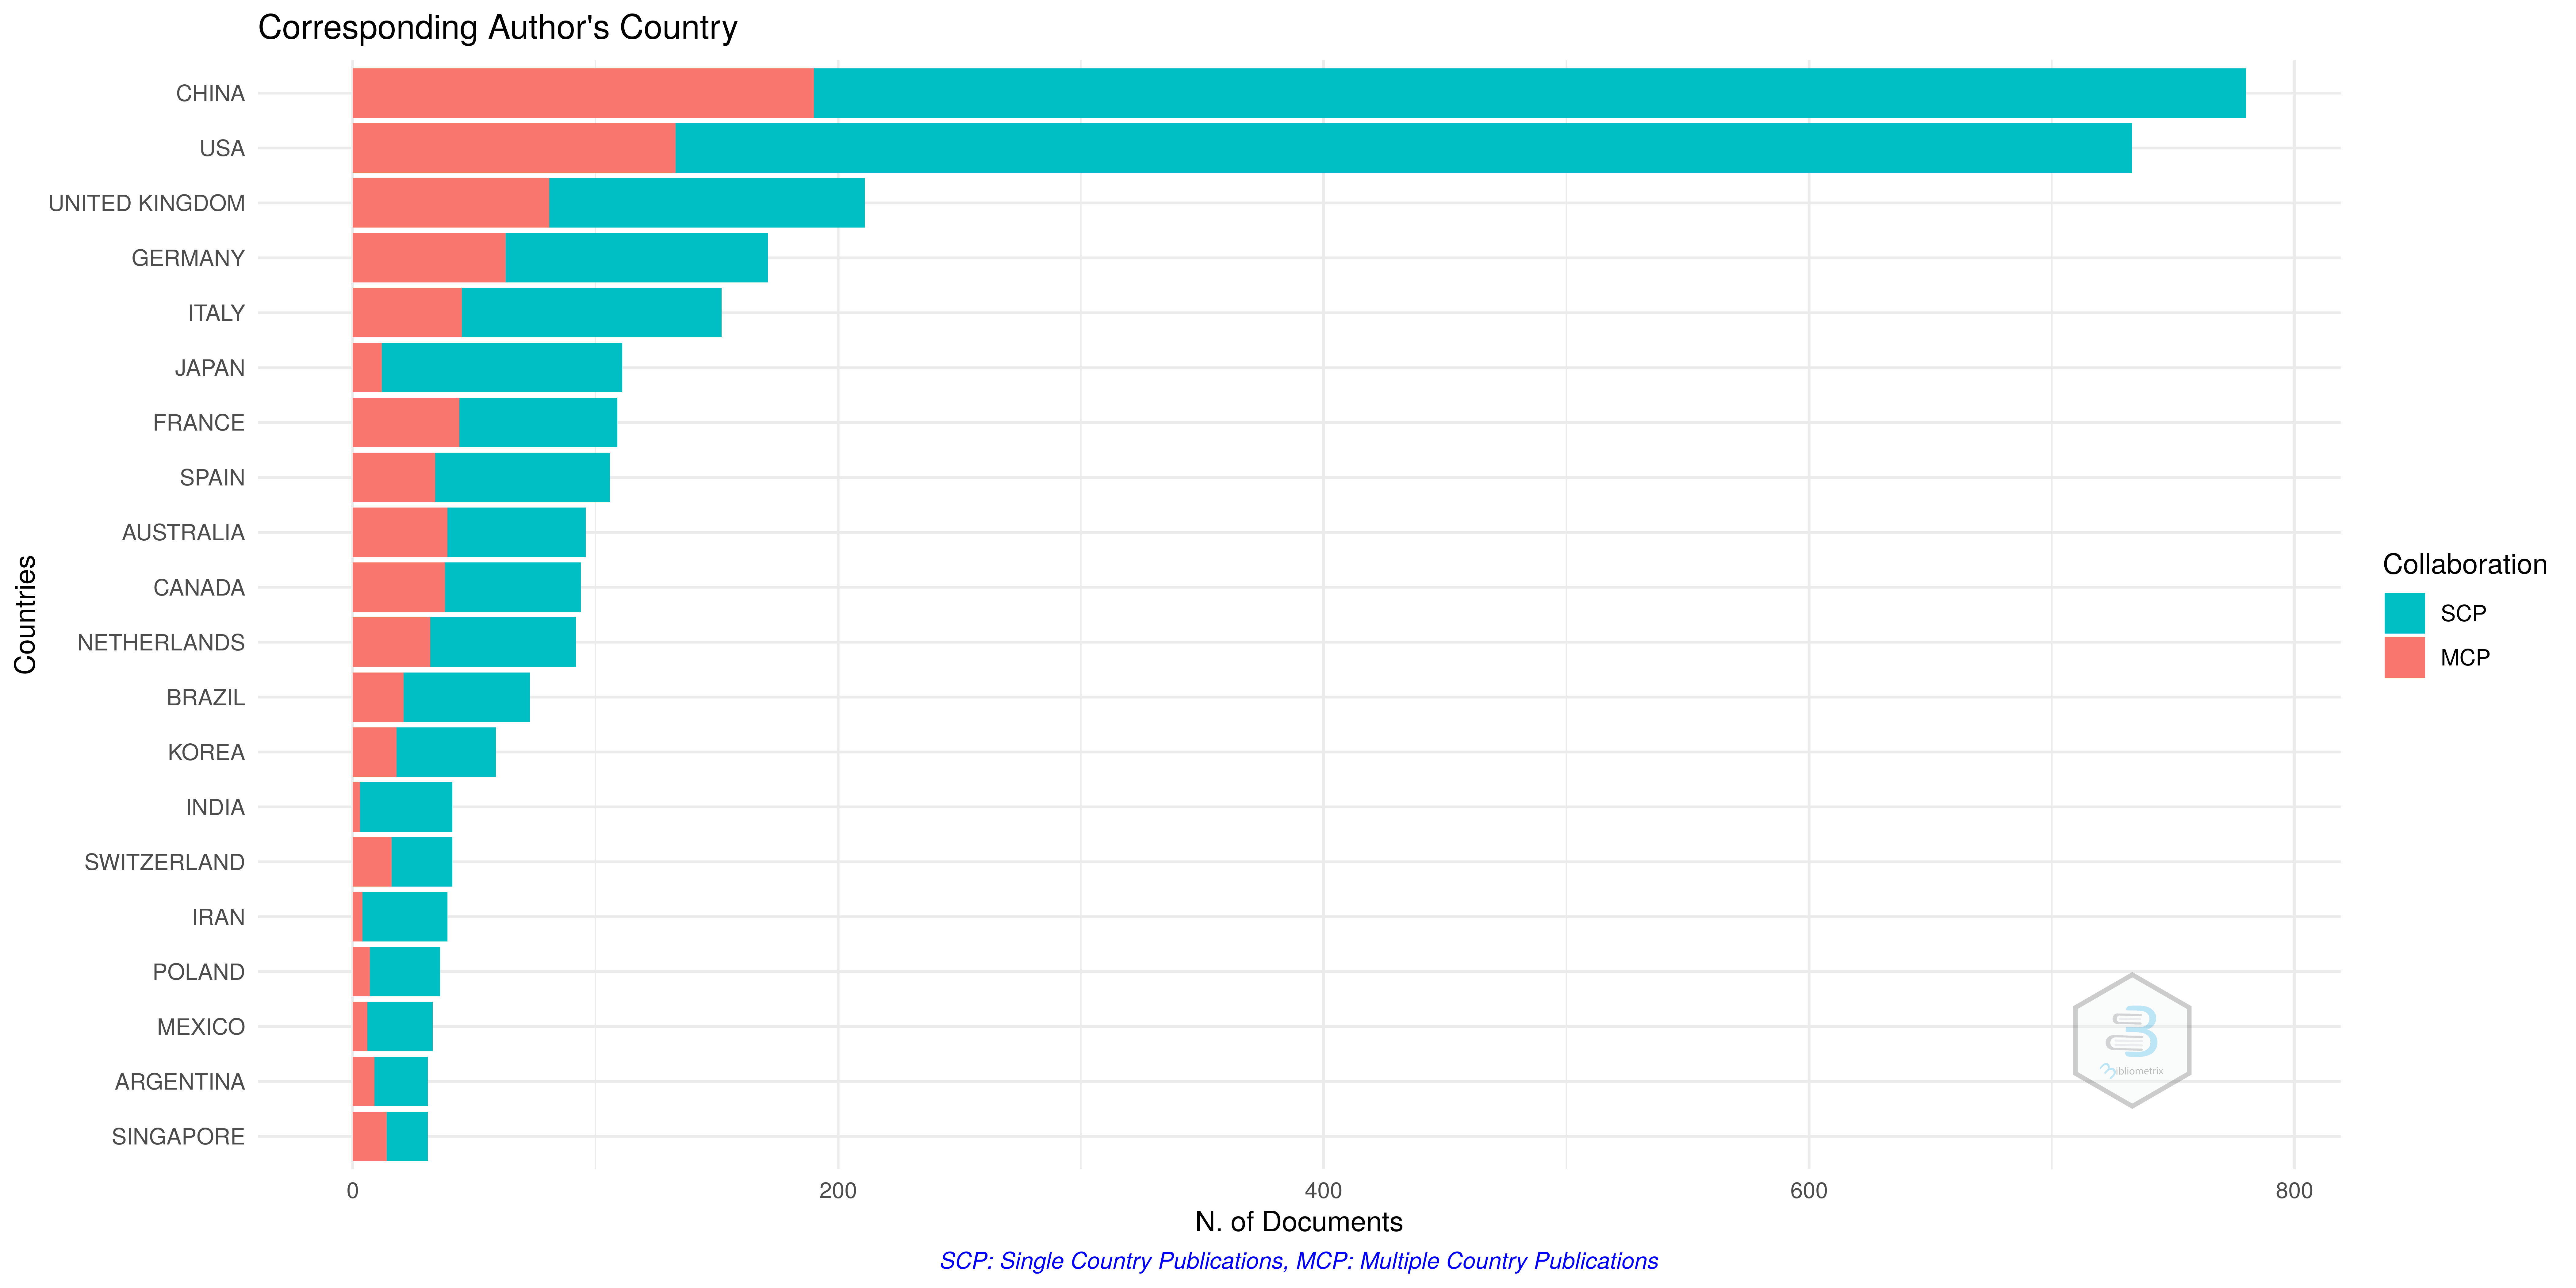
\includegraphics[angle=90,width=1\textwidth,height=0.93\textheight]{experiments/jhcf/PesqBibliogr/SimulacaoMultiagente/WoS-20220203/Metricas/Authors/MASSA2-Corresponding-Authors-Country.png}
    \caption{Variação da produção dos autores de maior impacto, do \dataset\ MASSA2@jhcf.}
    \label{fig:MASSA2-Corresponding-Authors-Country}
\end{figure}

\subsection{Métricas para Fontes de Informação}

As métricas para fontes de informação permitem avaliar a qualidade das revistas, conferências, em relação ao impacto de publicações em determinado tema. Valem a maioria das medidas já vistas para autores.

\subsubsection{Fontes mais relevantes, conforme número de artigos publicados sobre o tema}

\begin{figure}
    \centering
    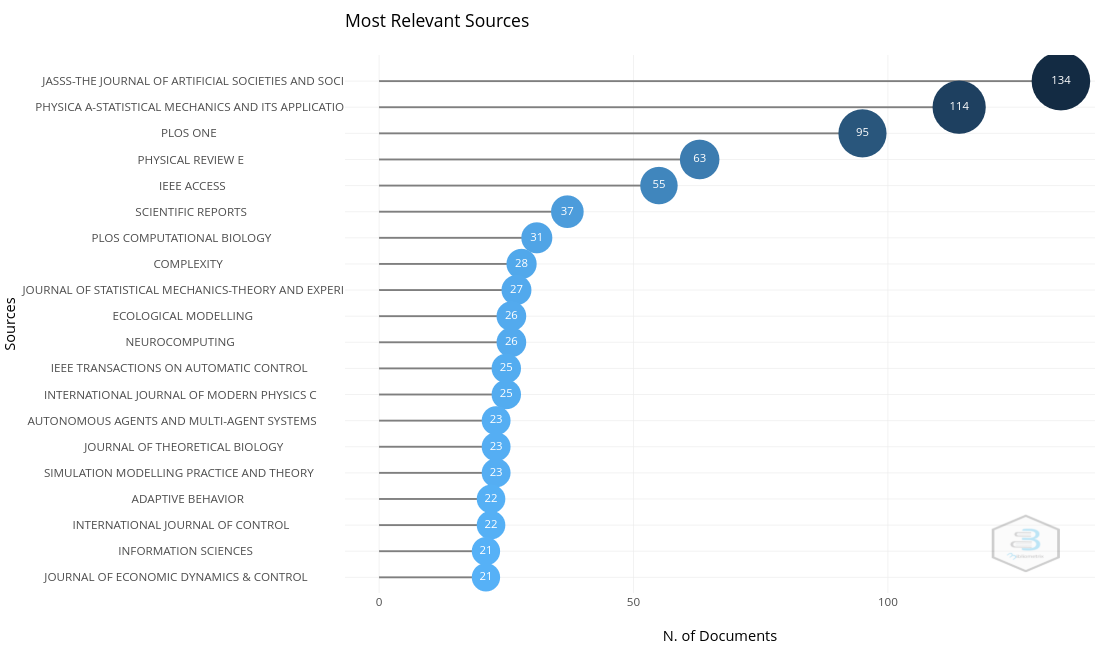
\includegraphics[width=1\textwidth]{experiments/jhcf/PesqBibliogr/SimulacaoMultiagente/WoS-20220203/Metricas/Sources/MASSA2-Most-Relevant-Sources.png}
    \caption{Revistas mais relevantes no  \dataset\ MASSA2@jhcf.}
    \label{fig:MASSA2-Most-Relevant-Sources}
\end{figure}

\subsubsection{Fontes mais relevantes, conforme o número de citações globais}

\begin{figure}
    \centering
    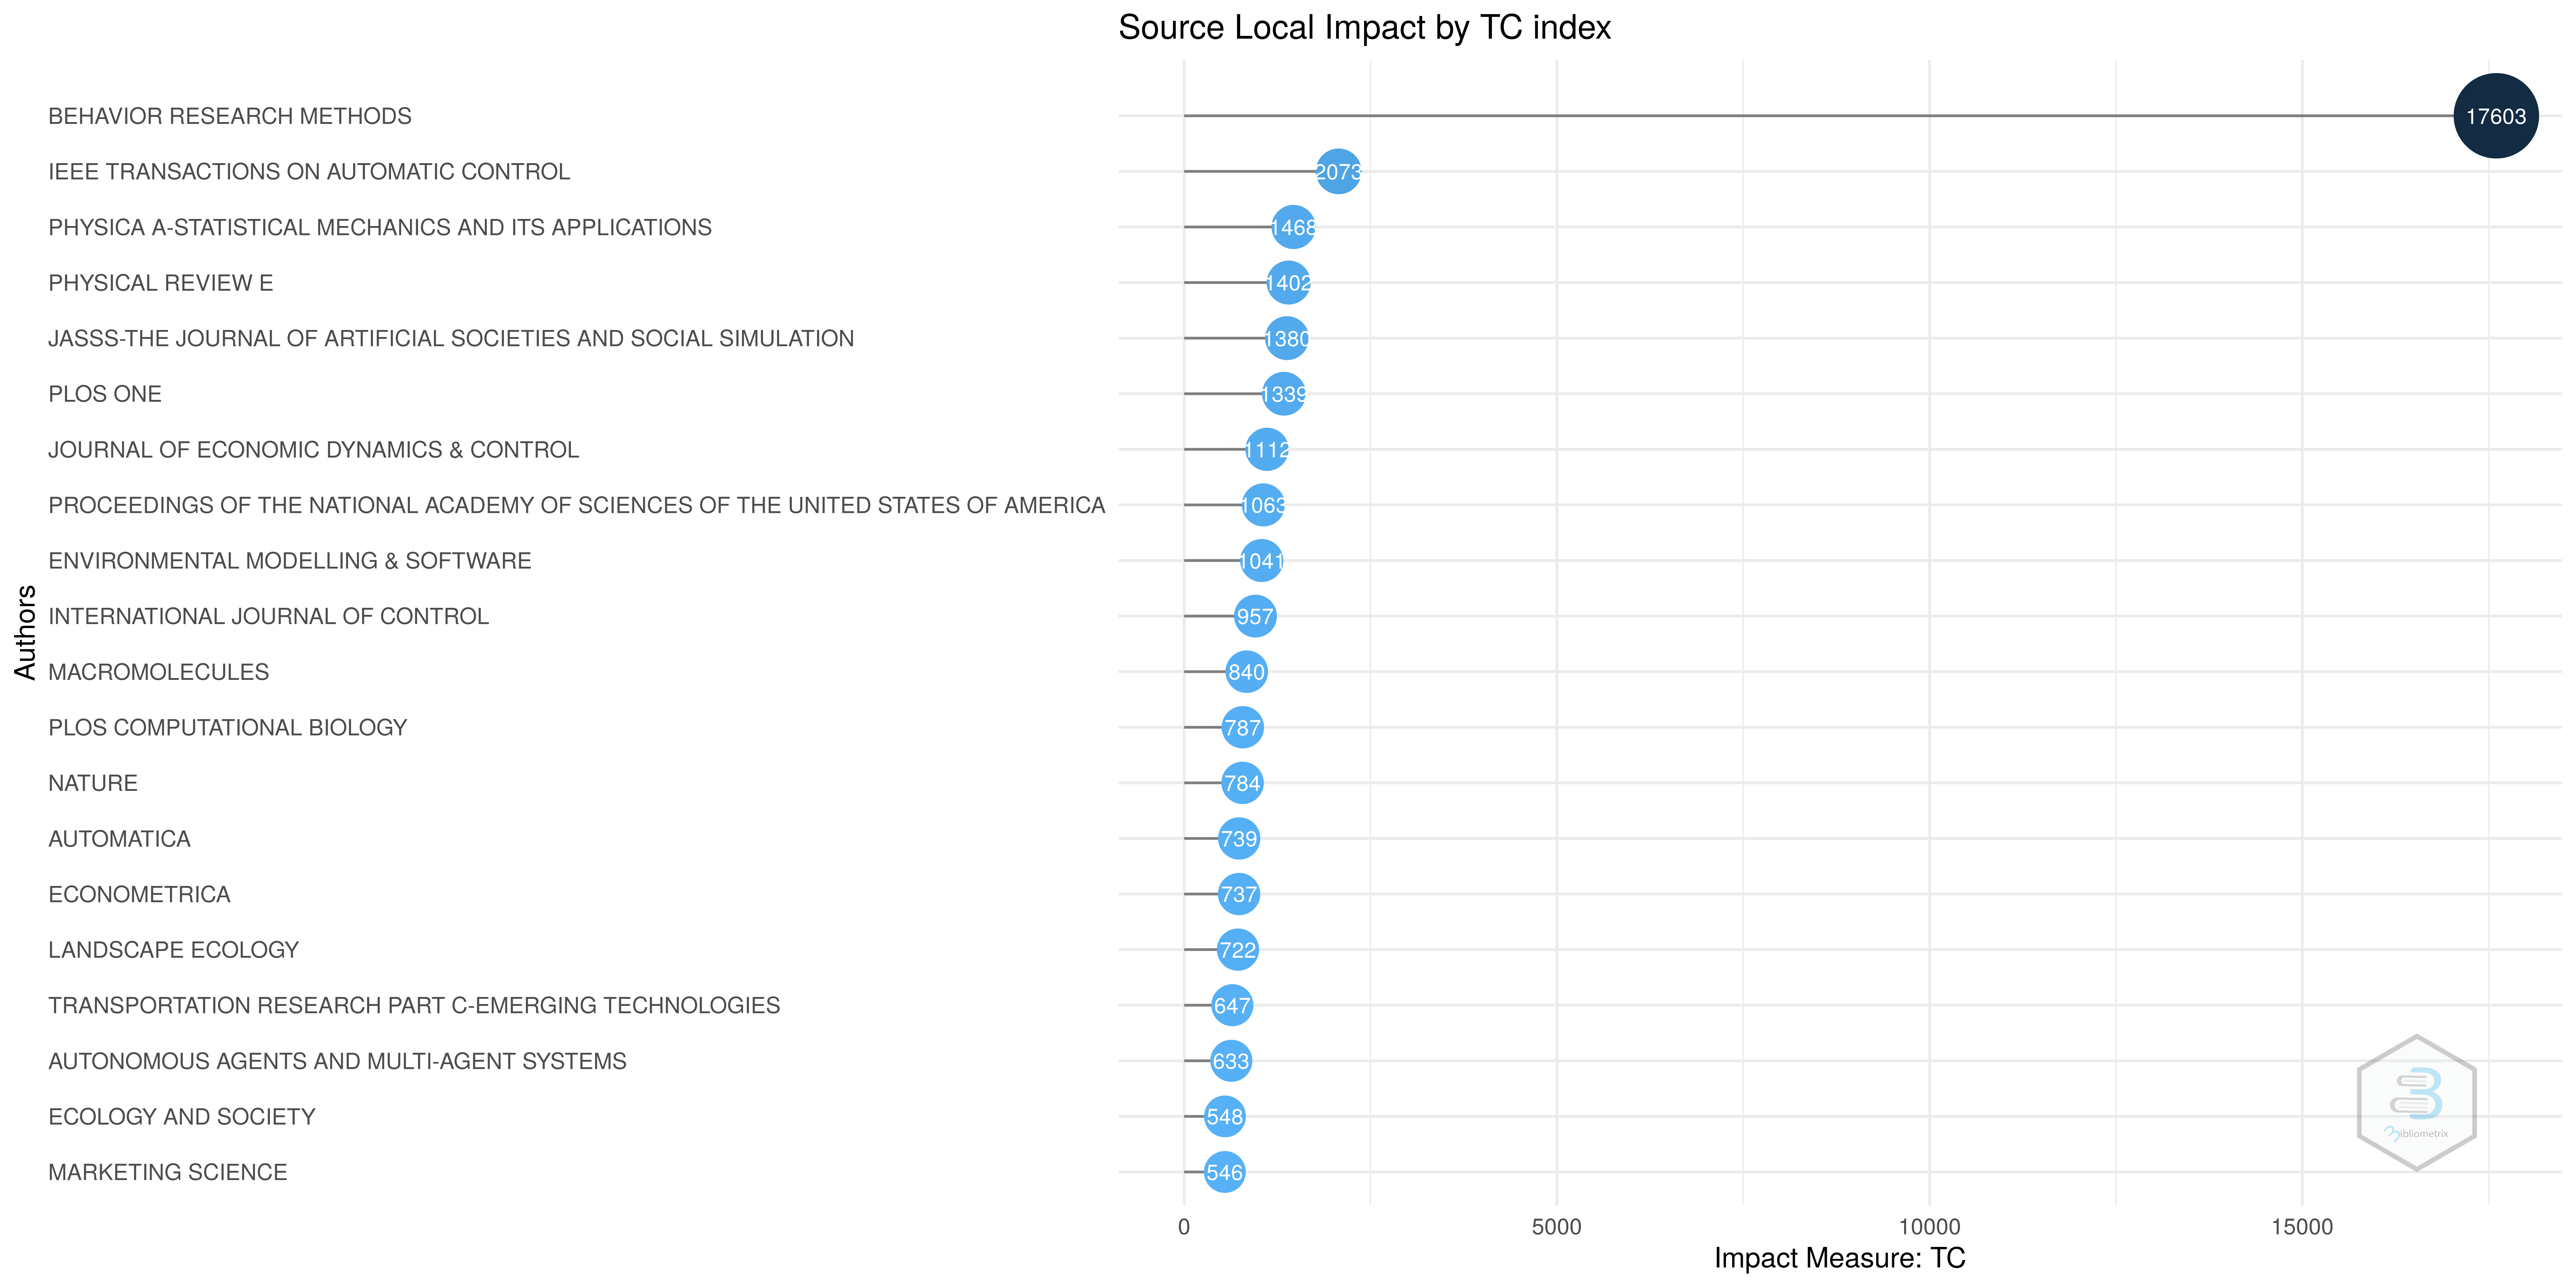
\includegraphics[width=1\textwidth]{experiments/jhcf/PesqBibliogr/SimulacaoMultiagente/WoS-20220203/Metricas/Sources/MASSA2-Total-Citation-Source-Local-Impact.png.png}
    \caption{Revistas mais relevantes no  \dataset\ MASSA2@jhcf, conforme a soma de citações aos artigos publicados.}
    \label{fig:MASSA2-Total-Citation-Source-Local-Impact.png}
\end{figure}

\subsubsection{Fontes mais relevantes, conforme o número de citações na lista de referências locais}

\begin{figure}
    \centering
    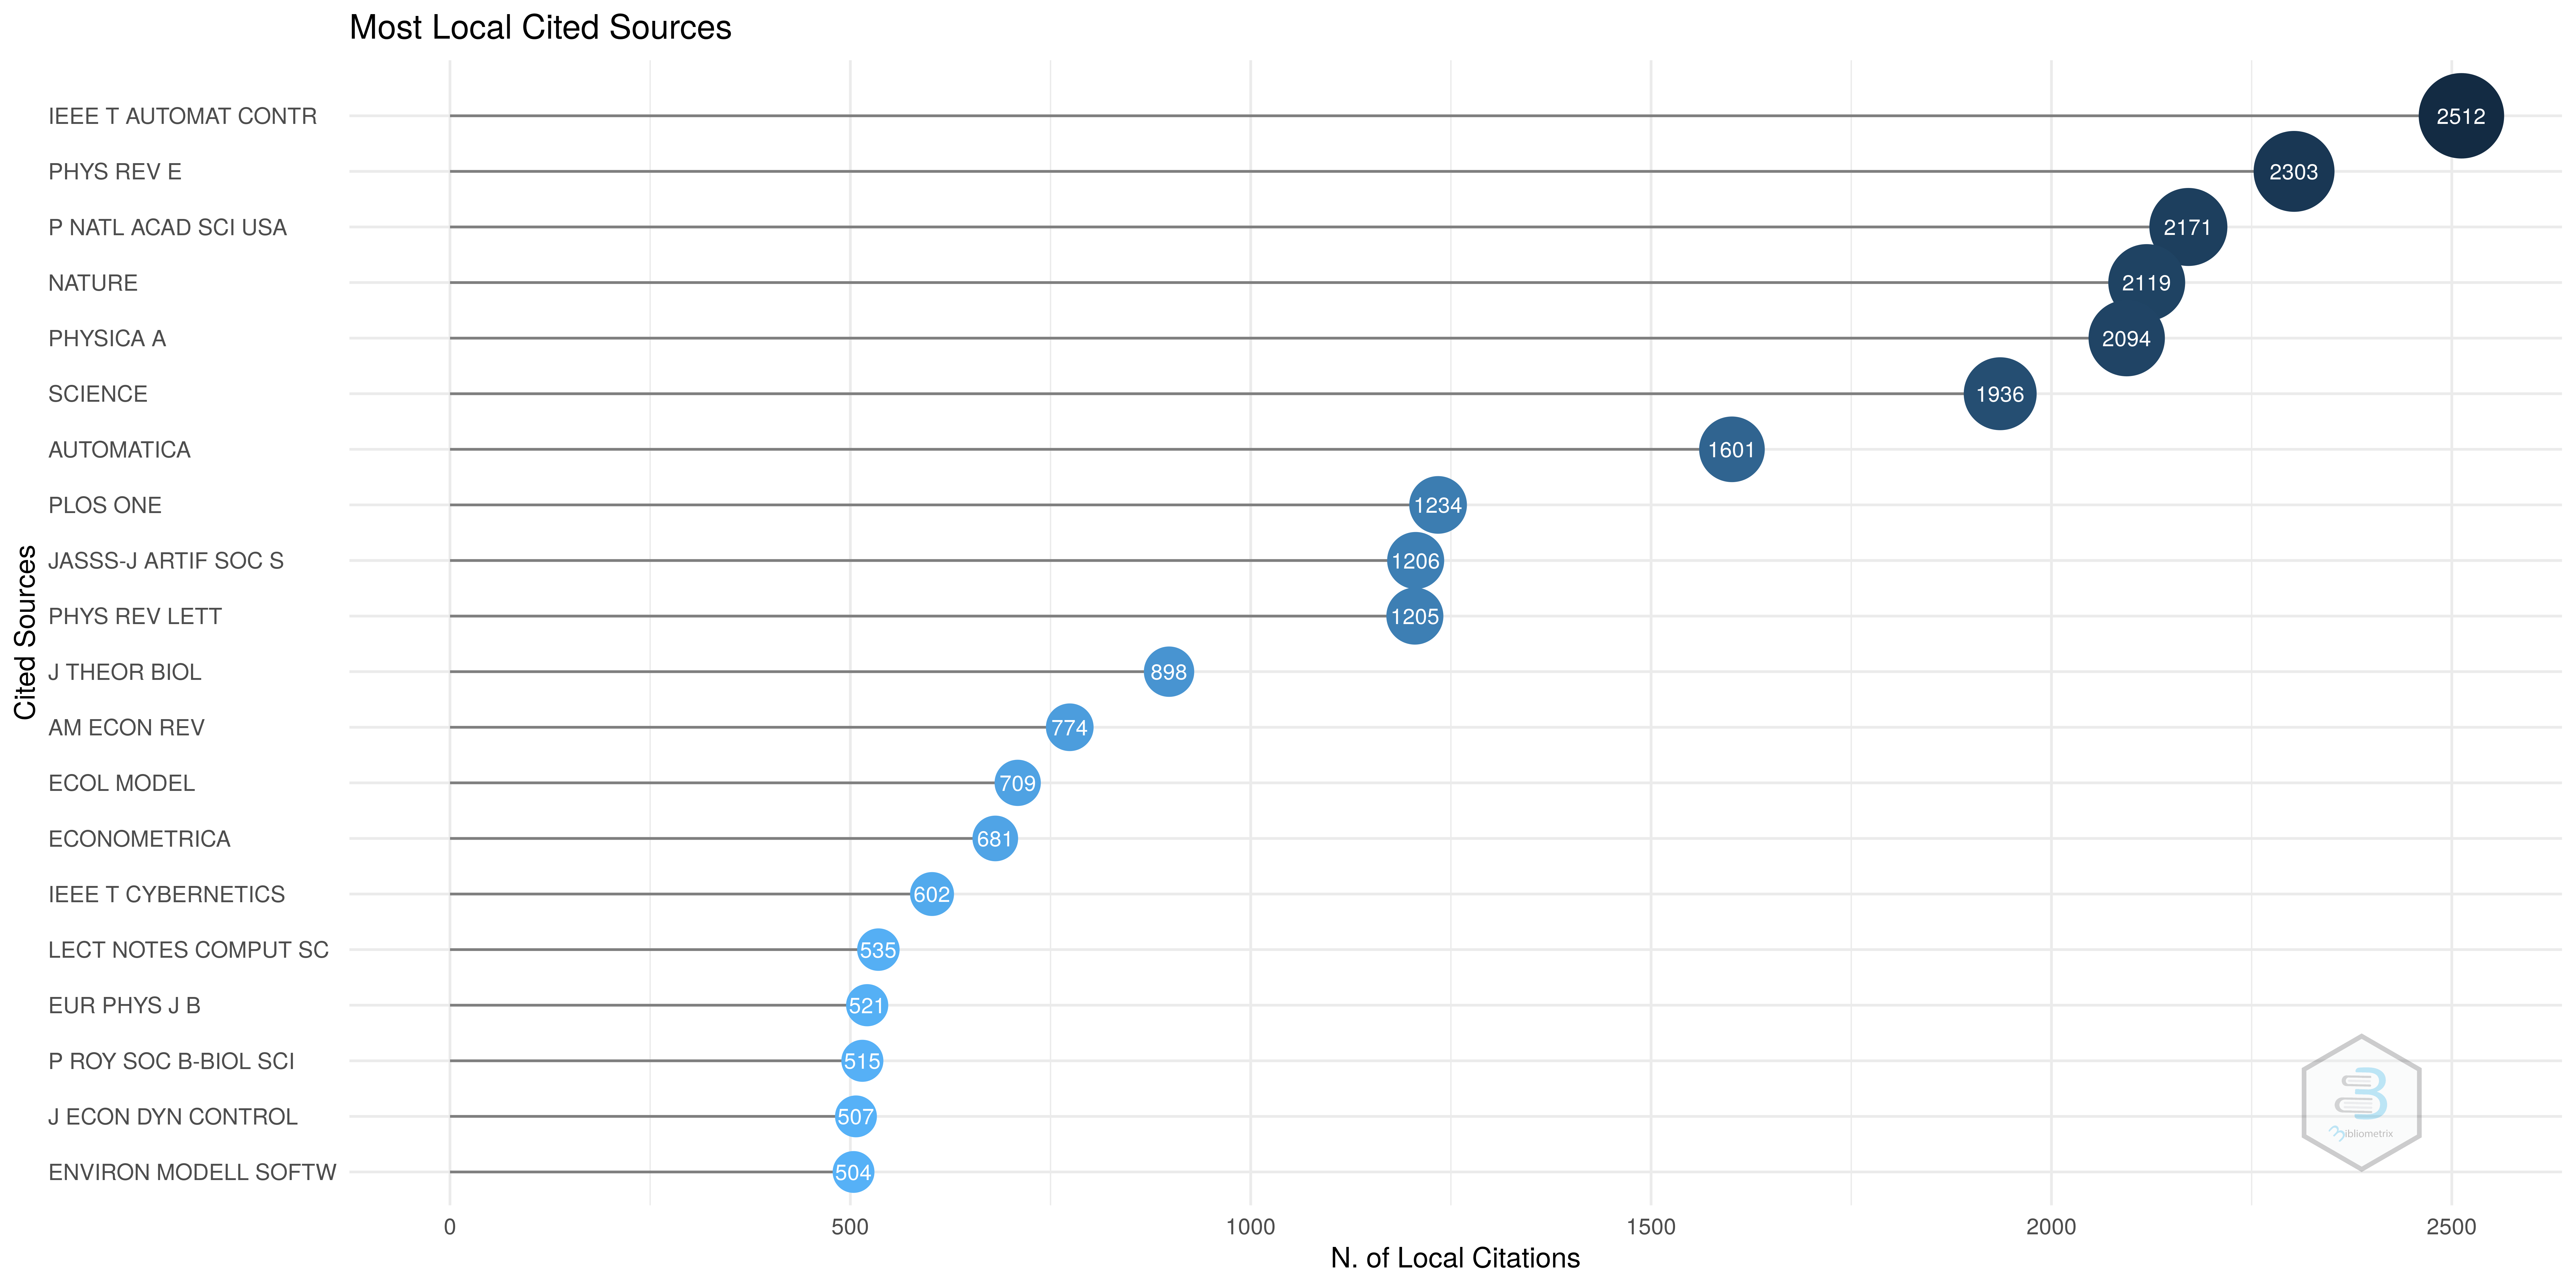
\includegraphics[width=1\textwidth]{experiments/jhcf/PesqBibliogr/SimulacaoMultiagente/WoS-20220203/Metricas/Sources/MASSA2-Most-Local-Cited-Sources(from-Reference-Lists).png}
    \caption{Revistas mais relevantes no  \dataset\ MASSA2@jhcf, conforme a soma de citações aos artigos no \dataset.}
    \label{fig:MASSA2-Most-Local-Cited-Sources(from-Reference-Lists).png}
\end{figure}

\subsubsection{Lei de Bradford}

\begin{figure}
    \centering
    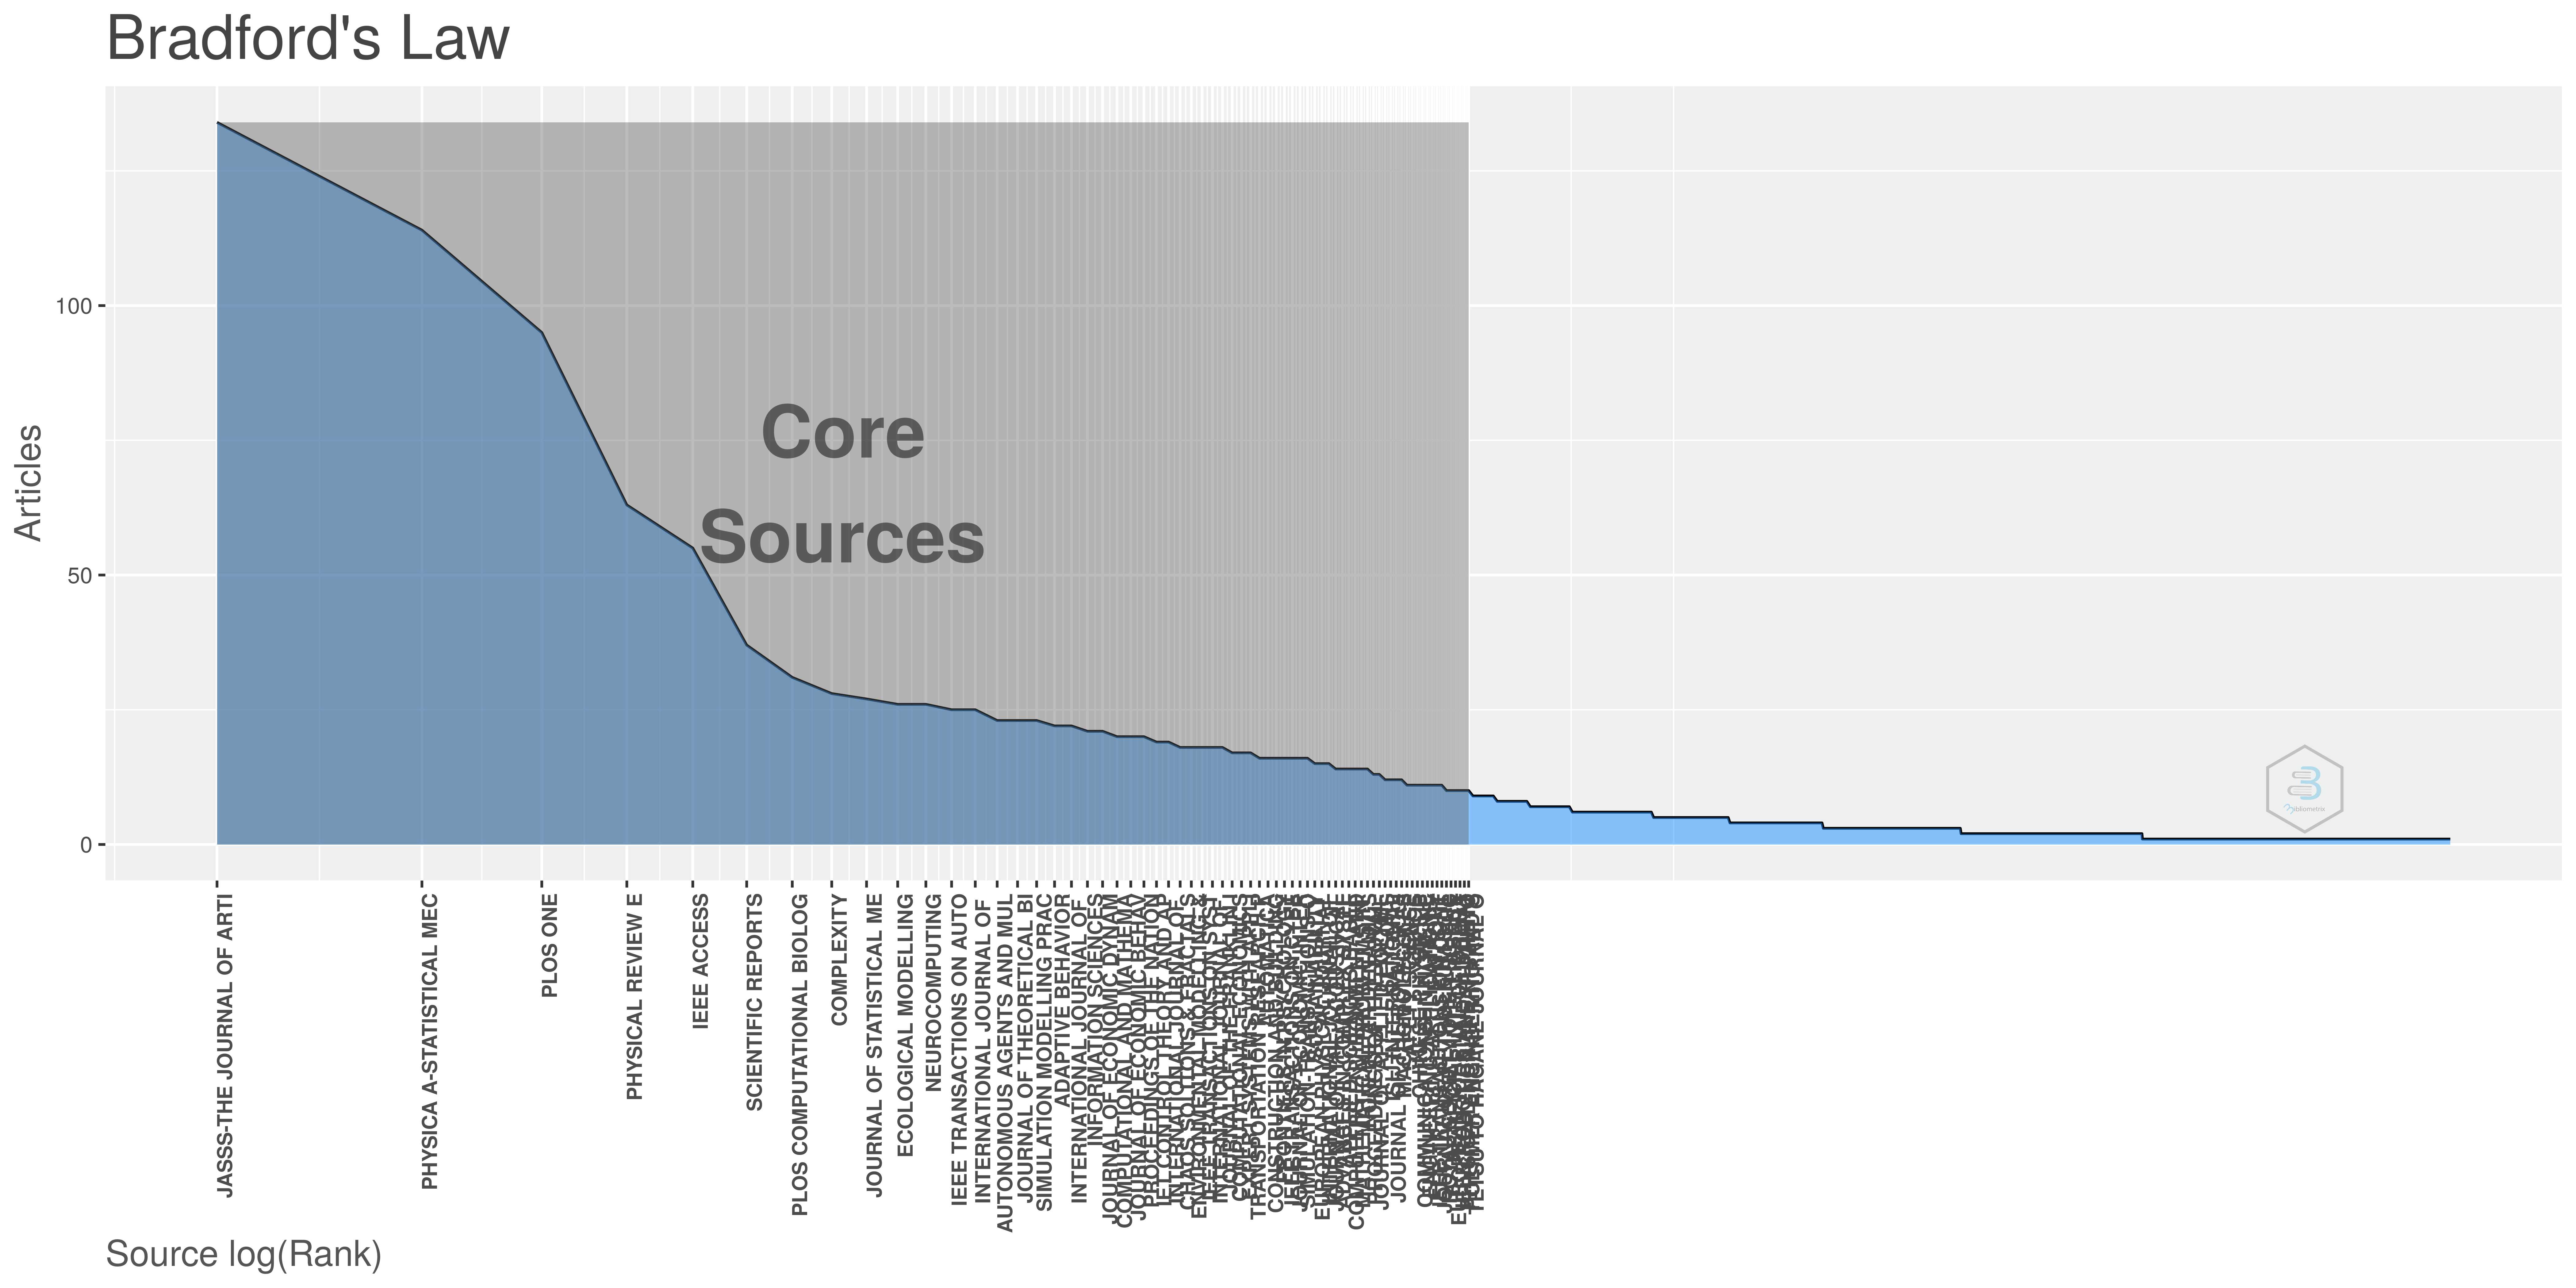
\includegraphics[width=1\textwidth]{experiments/jhcf/PesqBibliogr/SimulacaoMultiagente/WoS-20220203/Metricas/Sources/MASSA2-Bradfords-Law.png}
    \caption{Revistas mais relevantes no  \dataset\ MASSA2@jhcf, conforme a Lei de Bradford.}
    \label{fig:MASSA2-Bradfords-Law.png}
\end{figure}

\subsubsection{Medidas de Impacto das fontes}

\paragraph{Índice H}

\begin{figure}
    \centering
    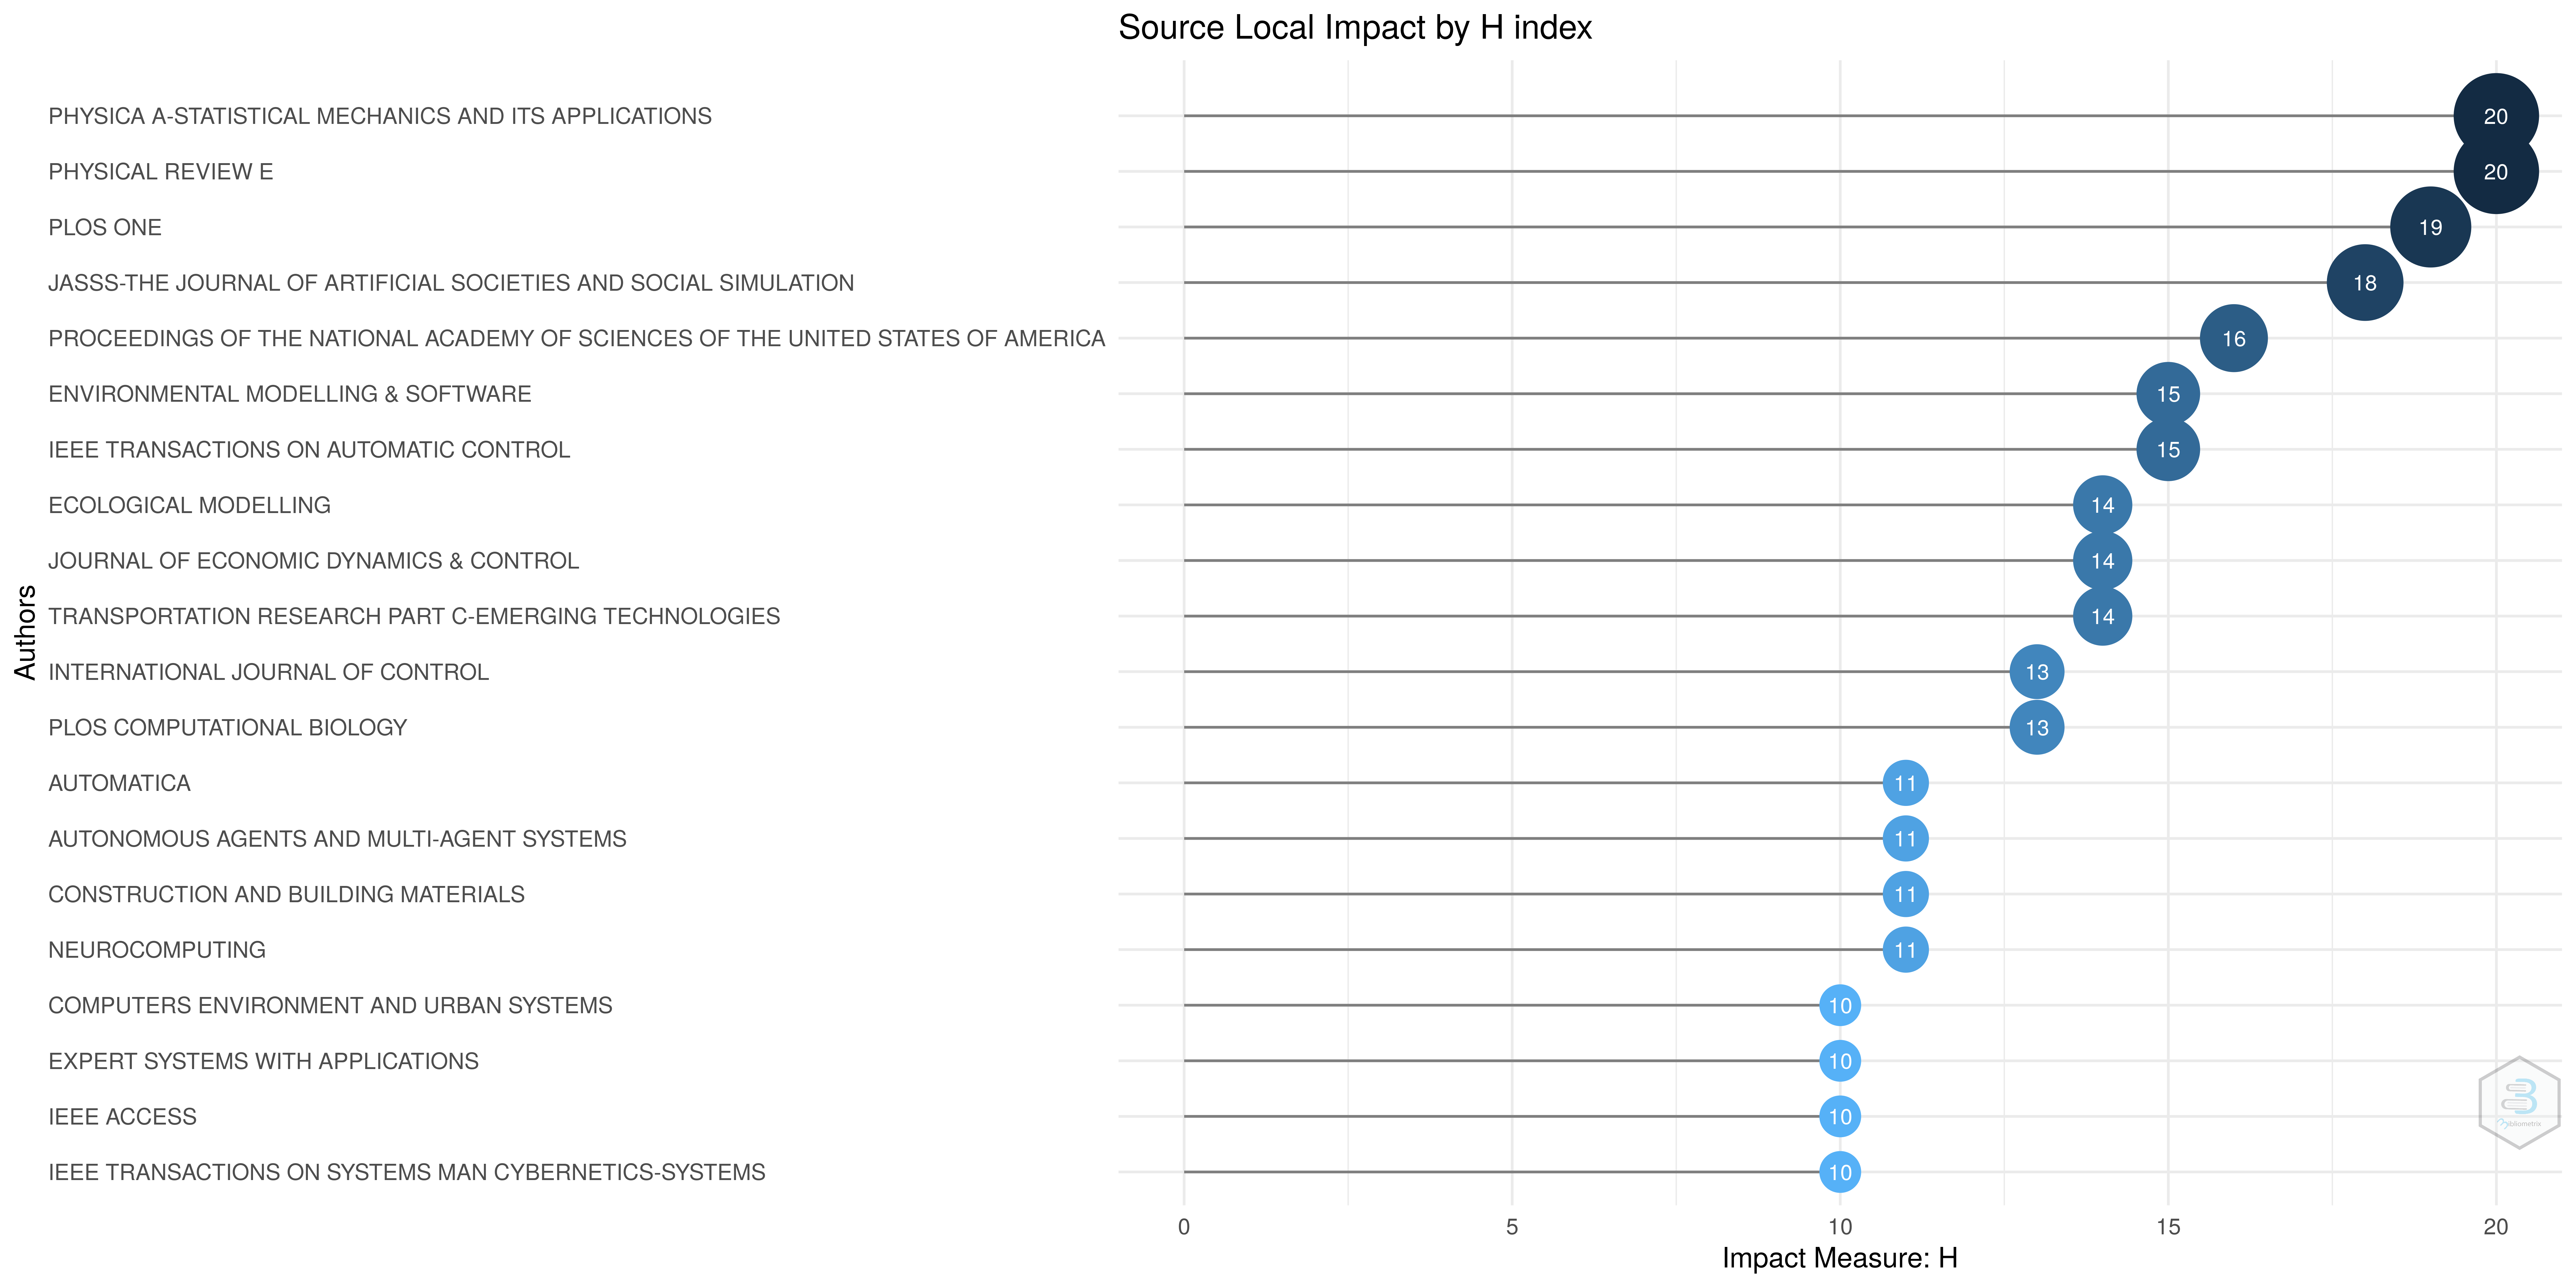
\includegraphics[width=1\textwidth]{experiments/jhcf/PesqBibliogr/SimulacaoMultiagente/WoS-20220203/Metricas/Sources/MASSA2-H-Index-Source-Local-Impact.png}
    \caption{Revistas de maior impacto no  \dataset\ MASSA2@jhcf,  conforme o índice H.}
    \label{fig:MASSA2-H-Index-Source-Local-Impact.png}
\end{figure}


\paragraph{Índice G}

\begin{figure}
    \centering
    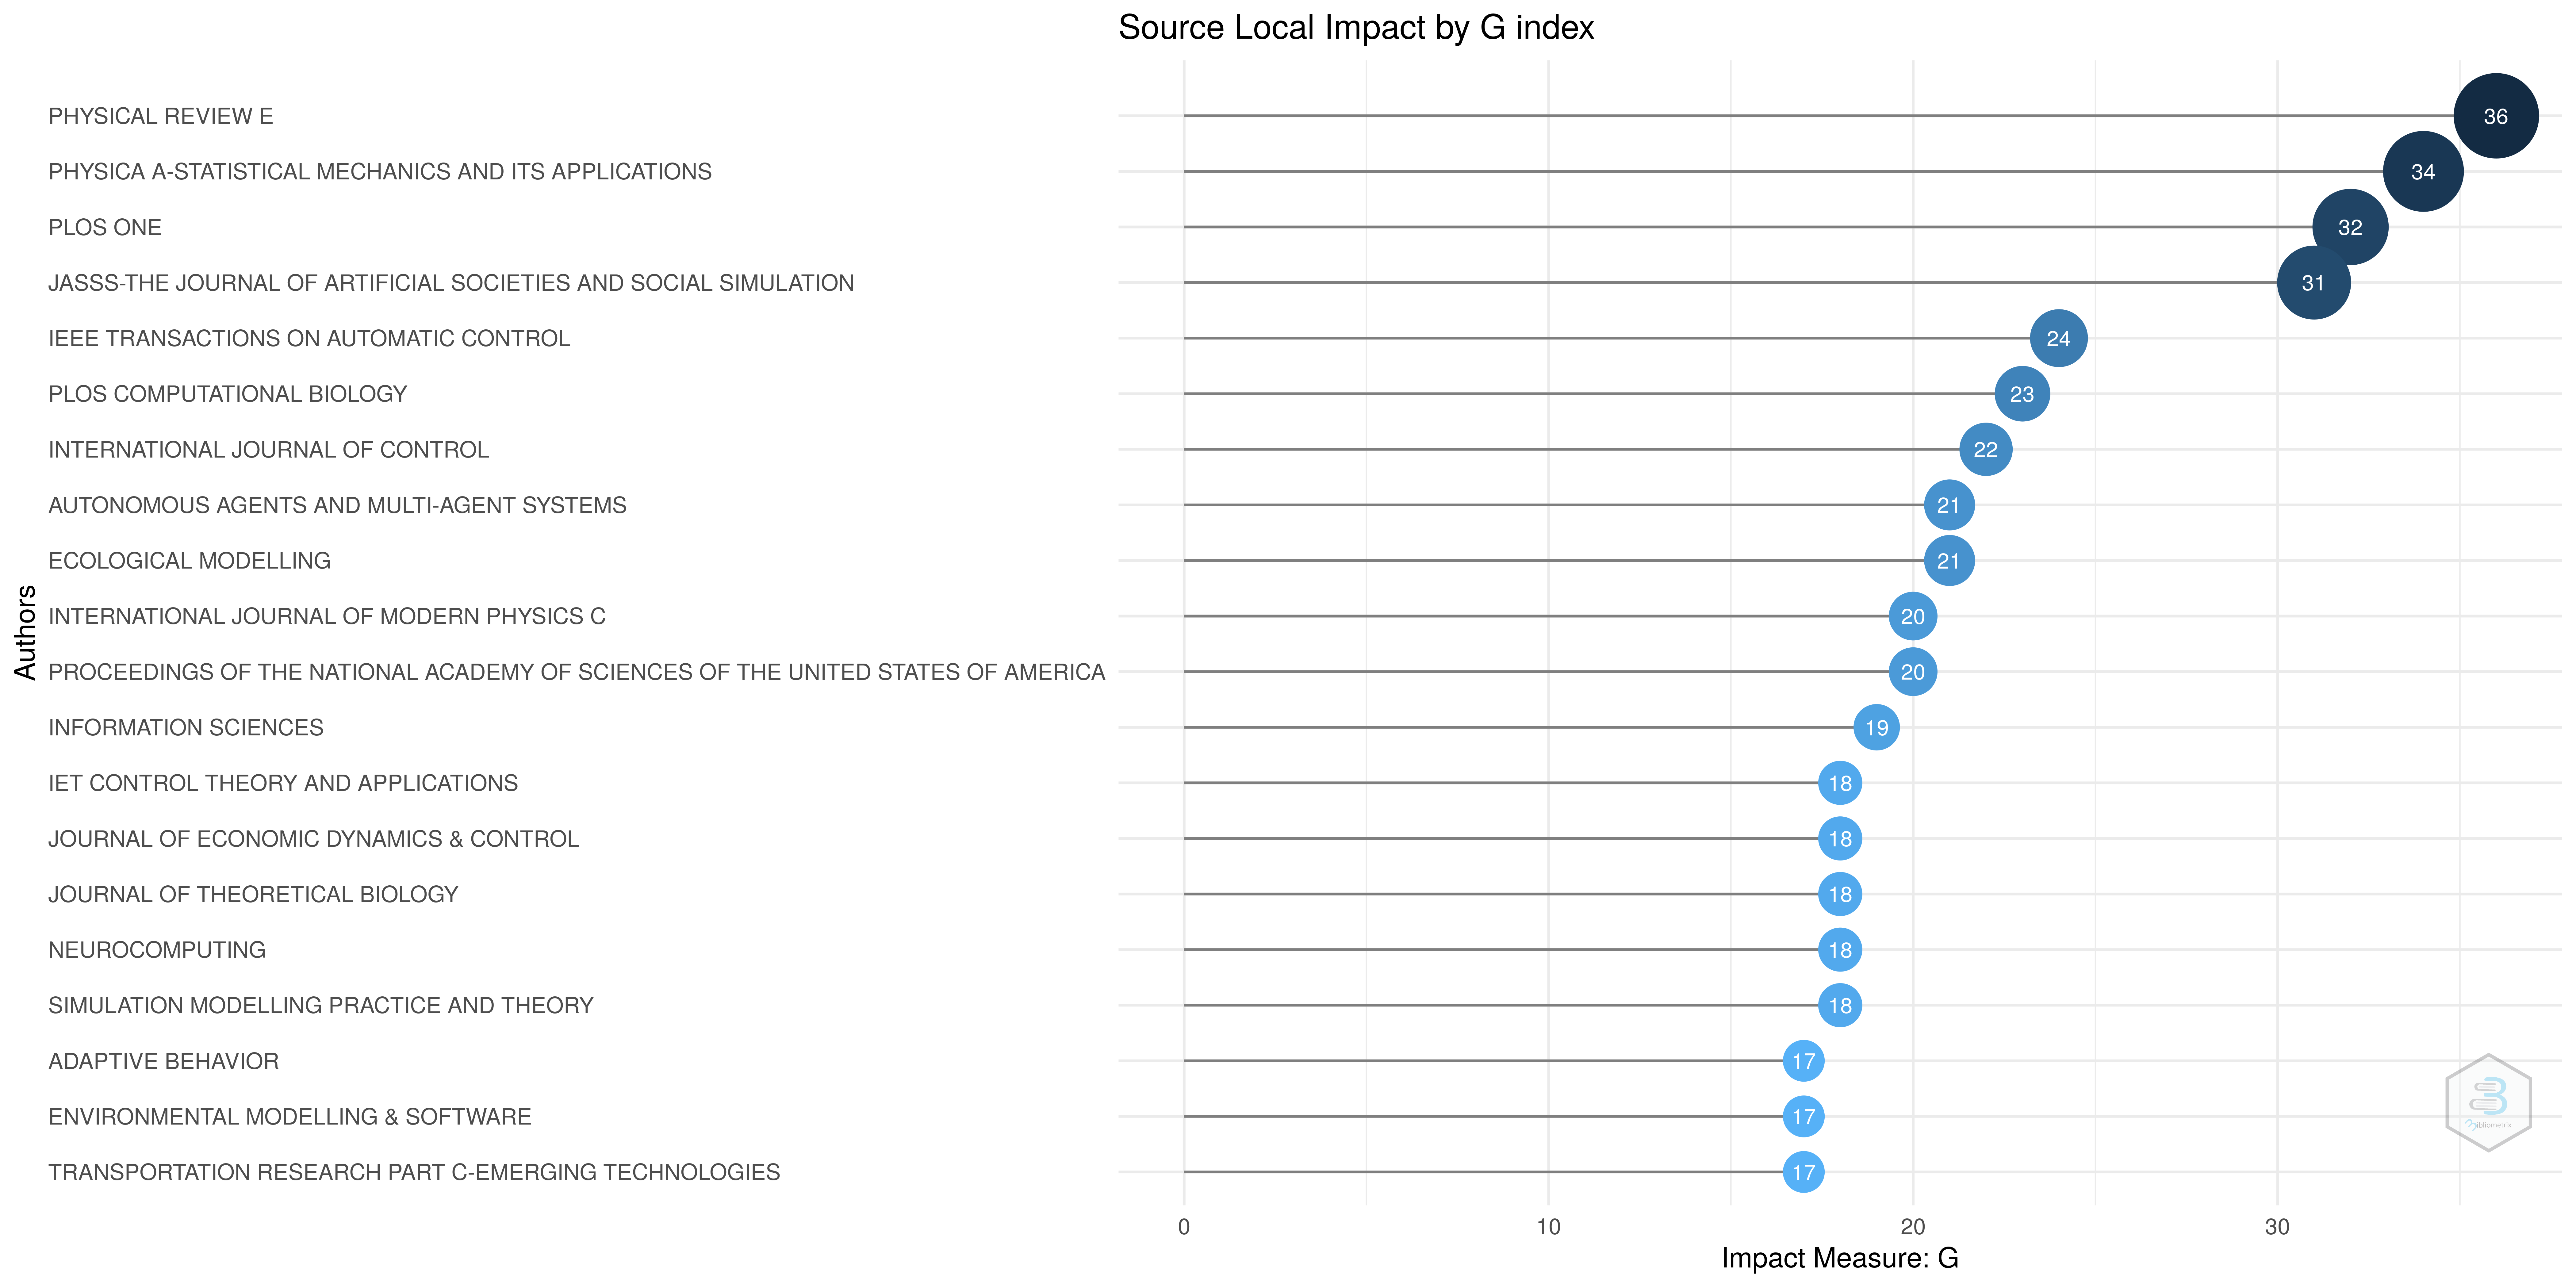
\includegraphics[width=1\textwidth]{experiments/jhcf/PesqBibliogr/SimulacaoMultiagente/WoS-20220203/Metricas/Sources/MASSA2-G-Index-Source-Local-Impact.png}
    \caption{Revistas de maior impacto no  \dataset\ MASSA2@jhcf,  conforme o índice G.}
    \label{fig:MASSA2-G-Index-Source-Local-Impact.png}
\end{figure}

\paragraph{Índice M}

\begin{figure}
    \centering
    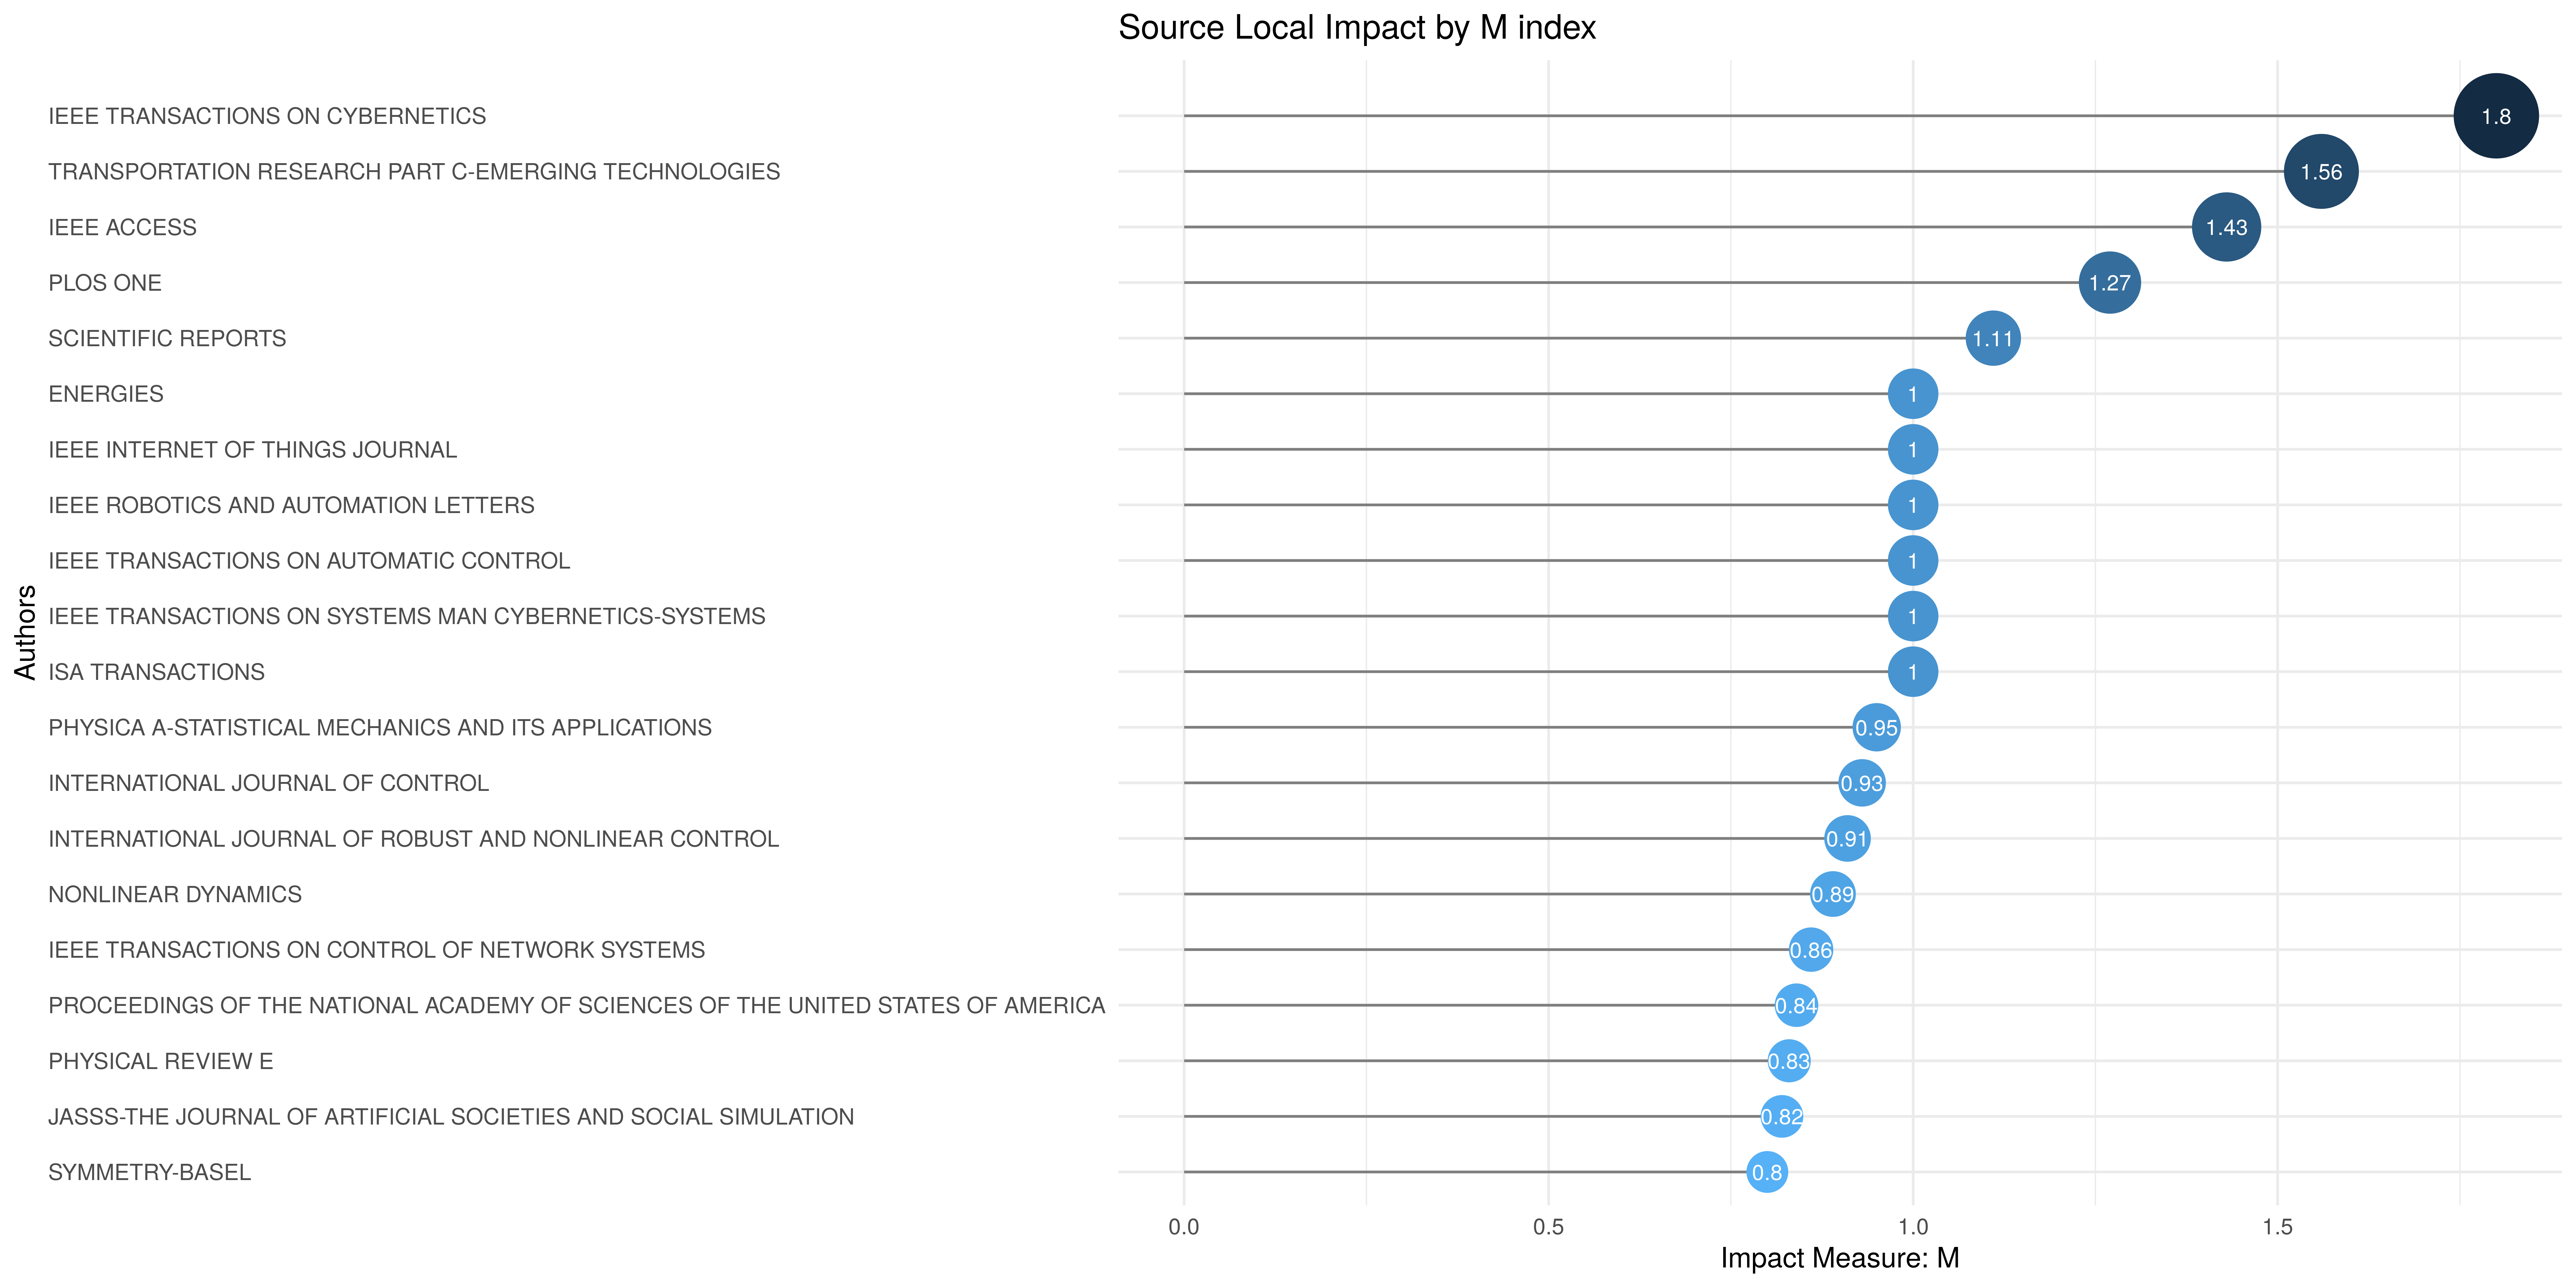
\includegraphics[width=1\textwidth]{experiments/jhcf/PesqBibliogr/SimulacaoMultiagente/WoS-20220203/Metricas/Sources/MASSA2-M-Index-Source-Local-Impact.png}
    \caption{Revistas de maior impacto no  \dataset\ MASSA2@jhcf,  conforme o índice M.}
    \label{fig:MASSA2-M-Index-Source-Local-Impact.png}
\end{figure}

\subsubsection{Dinâmica de publicação nas fontes}

\begin{figure}
    \centering
    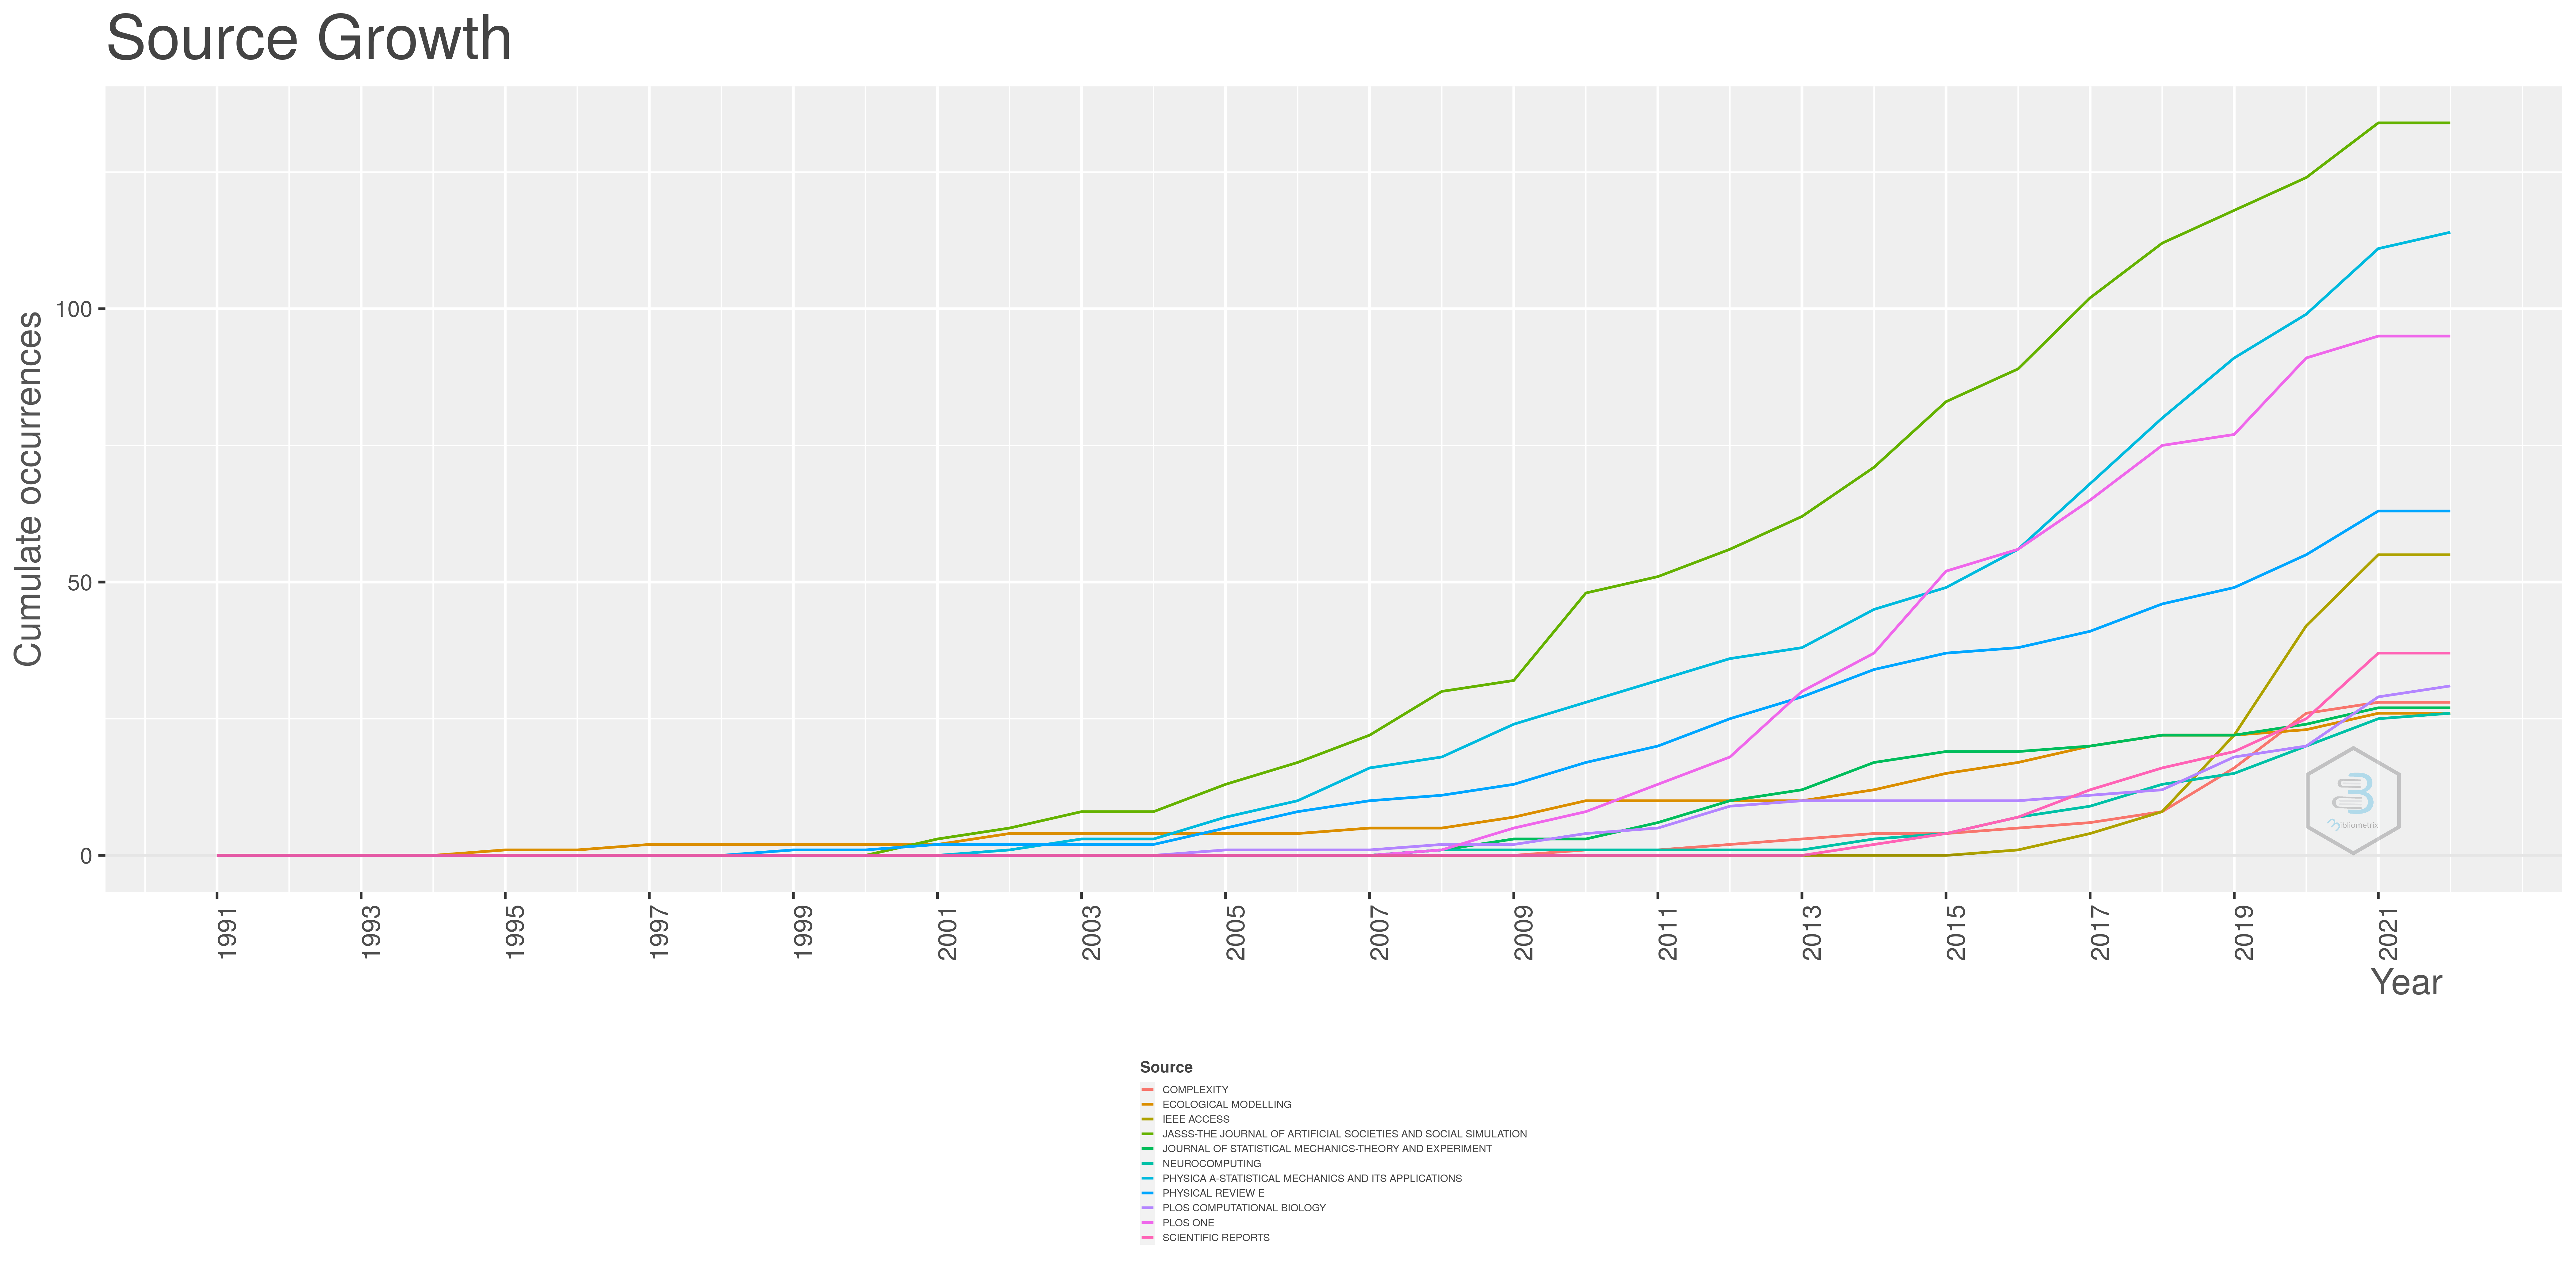
\includegraphics[width=1\textwidth]{experiments/jhcf/PesqBibliogr/SimulacaoMultiagente/WoS-20220203/Metricas/Sources/MASSA2-Source-Dynamics.png}
    \caption{Revistas com maior volume de publicações no tema no  \dataset\ MASSA2@jhcf, ao longo do tempo.}
    \label{fig:MASSA2-Source-Dynamics.png}
\end{figure}

\subsection{Mapas de Acoplamento}

\begin{figure}
    \centering
    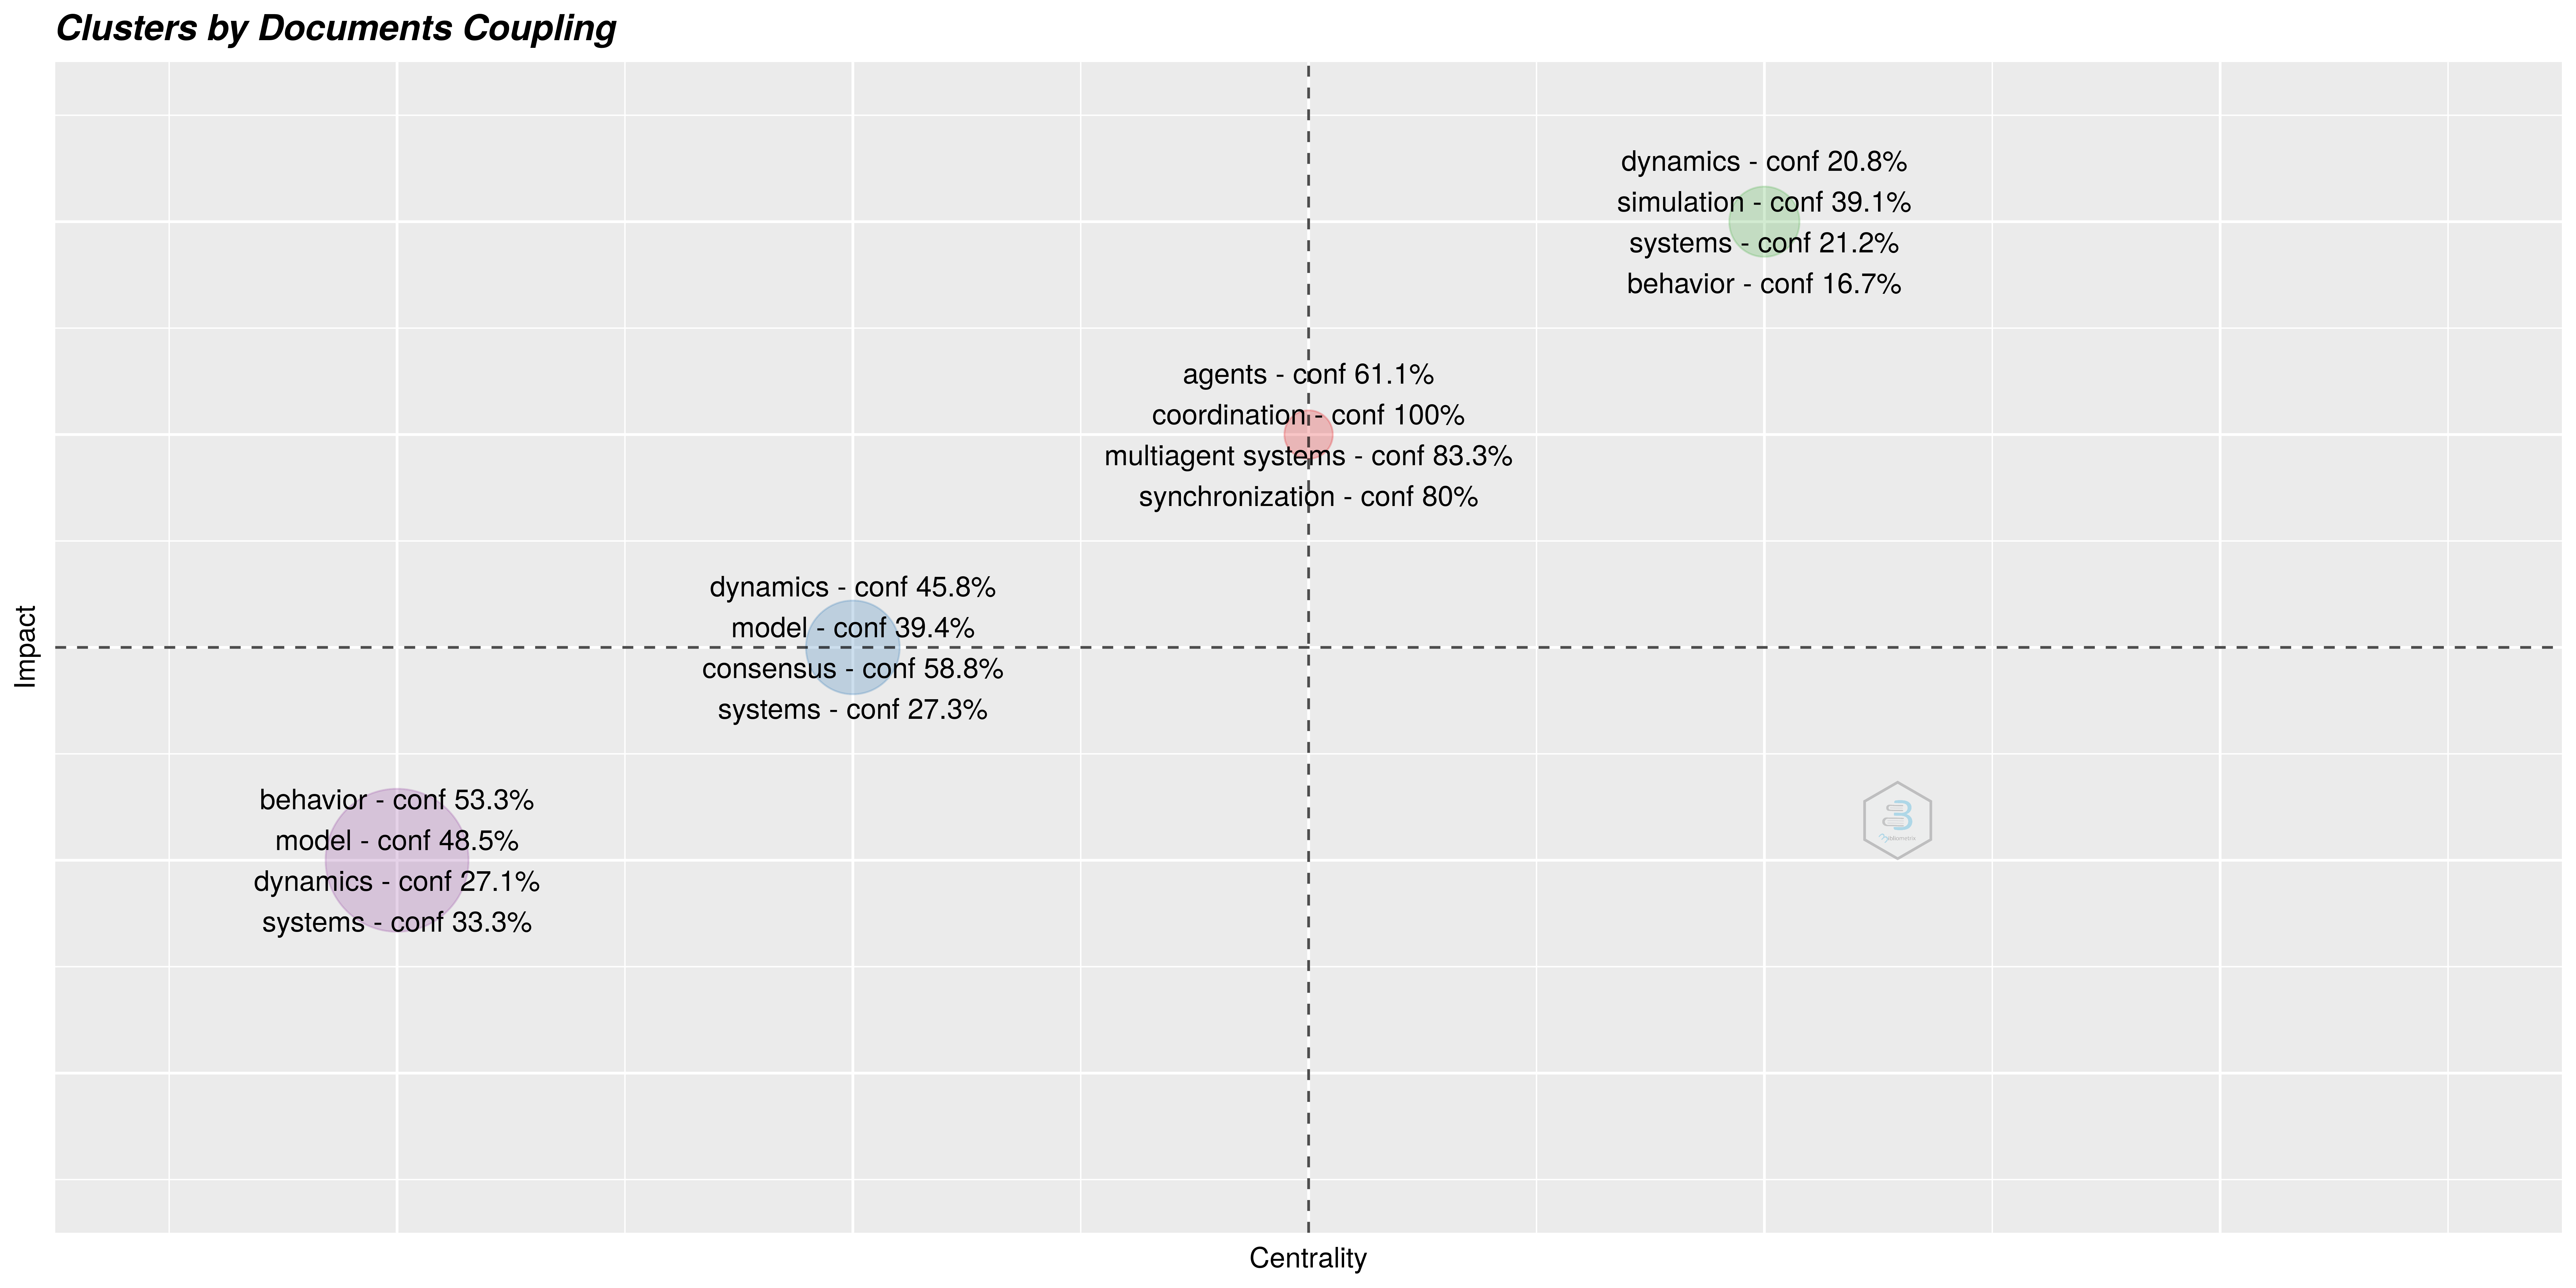
\includegraphics[width=1\textwidth]{experiments/jhcf/PesqBibliogr/SimulacaoMultiagente/WoS-20220203/Clustering/MASSA2-CouplingMap-4Labels-Per-Cluster.png}
    \caption{Palavras-chave mais evidentes que surgem nos clusters formados pelo Acoplamento bibliográfico entre documentos, no  \dataset\ MASSA2@jhcf.}
    \label{fig:MASSA2-CouplingMap-4Labels-Per-Cluster}
\end{figure}


\subsection{Estrutura Conceitual do Conhecimento}

O Conhecimento científico é um fenômeno complexo que emerge a partir da agregação memética de termos e palavras, que representam conceitos e ideias, que se organizam em tópicos, temas, e que evoluem ao longo do tempo (ver \url{https://en.wikipedia.org/wiki/Memetics}).

A estrutura conceitual do conhecimento pode ser produzida pela análise de relacionamento estabelecidos entre esses termos. O bibliometrix apresenta um conjunto de técnicas para evidenciar essa estrutura conceitual, e que se organizam em dois grupos:
\begin{description}
    \item [Métricas em rede] que usam grafos para representar relacionamentos entre termos, evidenciando, por meio de métricas de análise de redes sociais, como o conhecimento conceitualmente se organiza.
    \item [Análise Fatorial] Que emprega métricas de redução da dimensionalidade, para explorar, usualmente em mapas bidimensionais, como os termos e palavras se relacionam. 
\end{description}

\subsubsection{Métricas aplicadas a grafos (redes)}

\paragraph{Redes de Coocorrências}

As redes de coocorrências apresentam importantes padrões que se formam nas publicações, e podem revelar a estrutura conceitual de uma área do conhecimento.

No Biblioshiny quatro tipos de redes coocorrências podem ser geradas:
\begin{itemize}
    \item Baseadas na coocorrência de termos, revelando quais são os termos mais comumente citados 
\end{itemize}

\begin{figure}
    \centering
    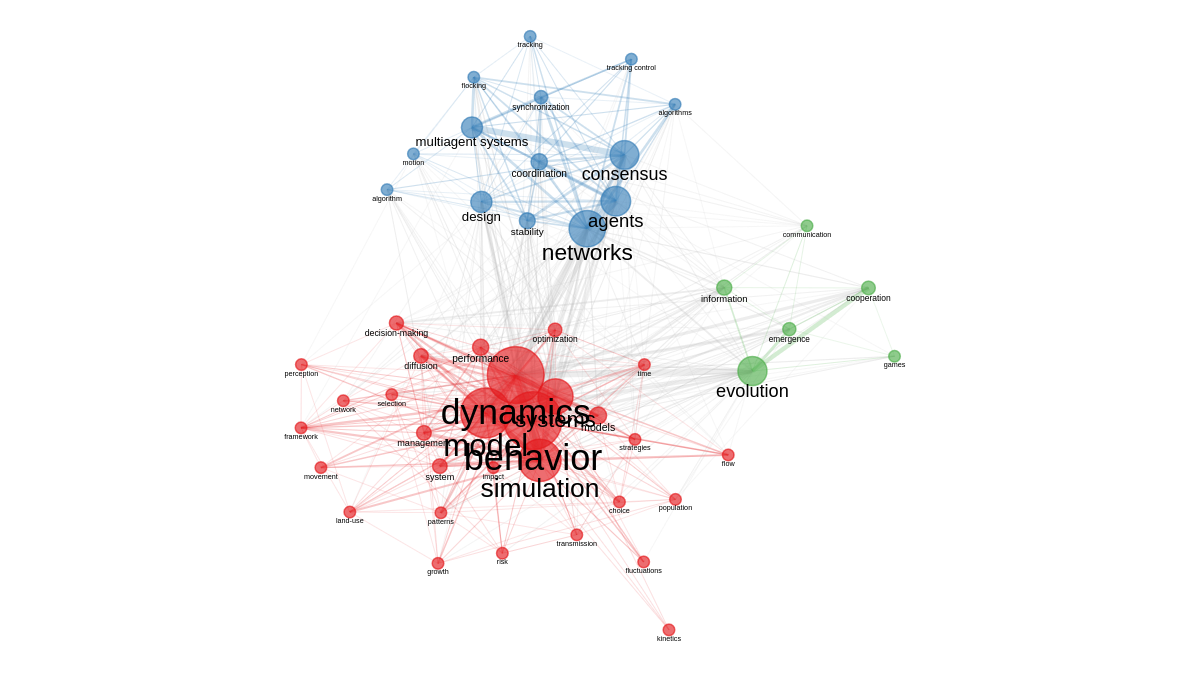
\includegraphics[width=1\textwidth]{experiments/jhcf/PesqBibliogr/SimulacaoMultiagente/WoS-20220203/Estrutura/Conceitual/MASSA2-Co-occurrence-Network-50nodes-louvainclustering.png.png}
    \caption{50 palavras-chave mais evidentes, clusterizadas pela coocorrência em documentos, no  \dataset\ MASSA2@jhcf.}
    \label{fig:MASSA2-Co-occurrence-Network-50nodes-louvainclustering.png}
\end{figure}

\begin{figure}
    \centering
    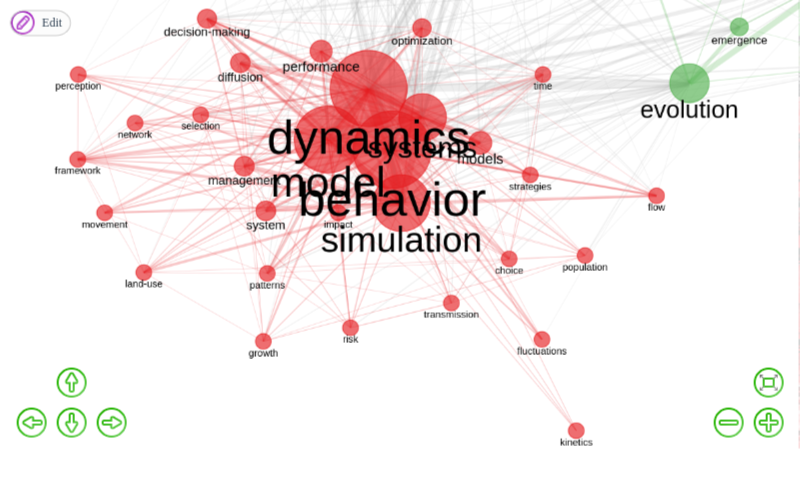
\includegraphics[width=1\textwidth]{experiments/jhcf/PesqBibliogr/SimulacaoMultiagente/WoS-20220203/Estrutura/Conceitual/MASSA2-Cluster1-Co-occurrence-Network-50nodes-louvainclustering.png.png}
    \caption{Detalhamento do cluster 1, na rede das 50 palavras-chave mais evidentes, clusterizadas pela coocorrência em documentos, no  \dataset\ MASSA2@jhcf.}
    \label{fig:MASSA2-Cluster1-Co-occurrence-Network-50nodes-louvainclustering.png}
\end{figure}

\begin{figure}
    \centering
    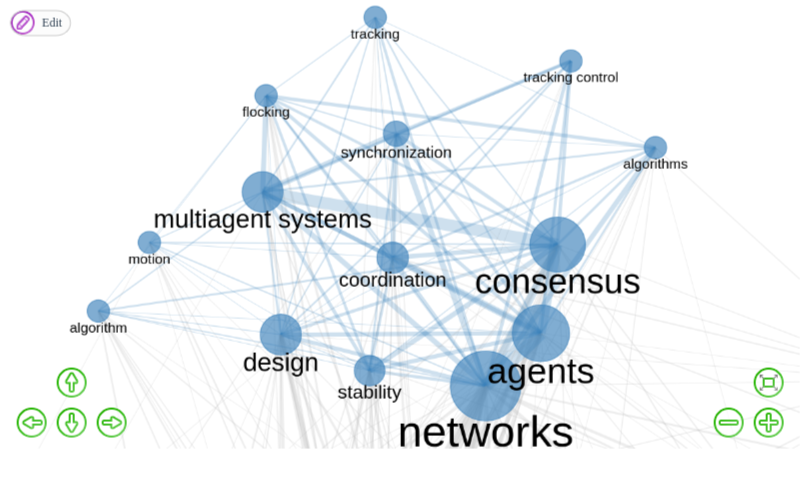
\includegraphics[width=1\textwidth]{experiments/jhcf/PesqBibliogr/SimulacaoMultiagente/WoS-20220203/Estrutura/Conceitual/MASSA2-Cluster2-Co-occurrence-Network-50nodes-louvainclustering.png.png.png}
    \caption{Detalhamento do cluster 2, na rede das 50 palavras-chave mais evidentes, clusterizadas pela coocorrência em documentos, no  \dataset\ MASSA2@jhcf.}
    \label{fig:MASSA2-Cluster2-Co-occurrence-Network-50nodes-louvainclustering.png.png}
\end{figure}

\begin{figure}
    \centering
    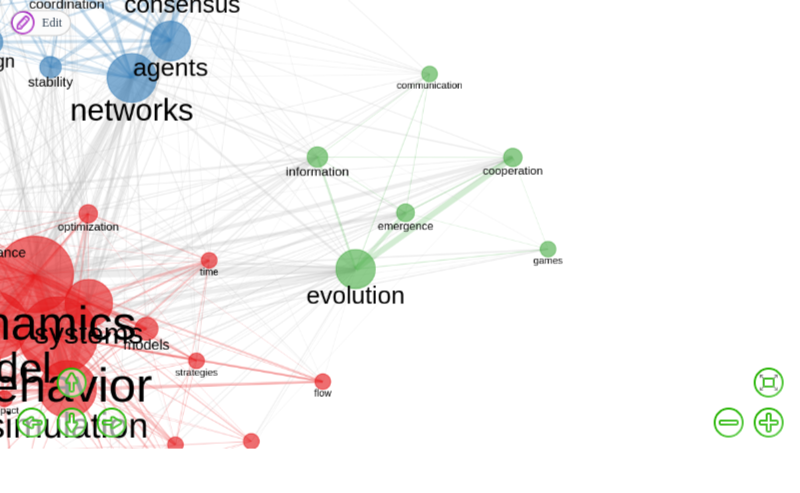
\includegraphics[width=1\textwidth]{experiments/jhcf/PesqBibliogr/SimulacaoMultiagente/WoS-20220203/Estrutura/Conceitual/MASSA2-Cluster3-Co-occurrence-Network-50nodes-louvainclustering.png.png.png}
    \caption{Detalhamento do cluster 3, na rede das 50 palavras-chave mais evidentes, clusterizadas pela coocorrência em documentos, no  \dataset\ MASSA2@jhcf.}
    \label{fig:MASSA2-Cluster3-Co-occurrence-Network-50nodes-louvainclustering.png.png}
\end{figure}

\paragraph{Mapas Temáticos}

\begin{figure}
    \centering
    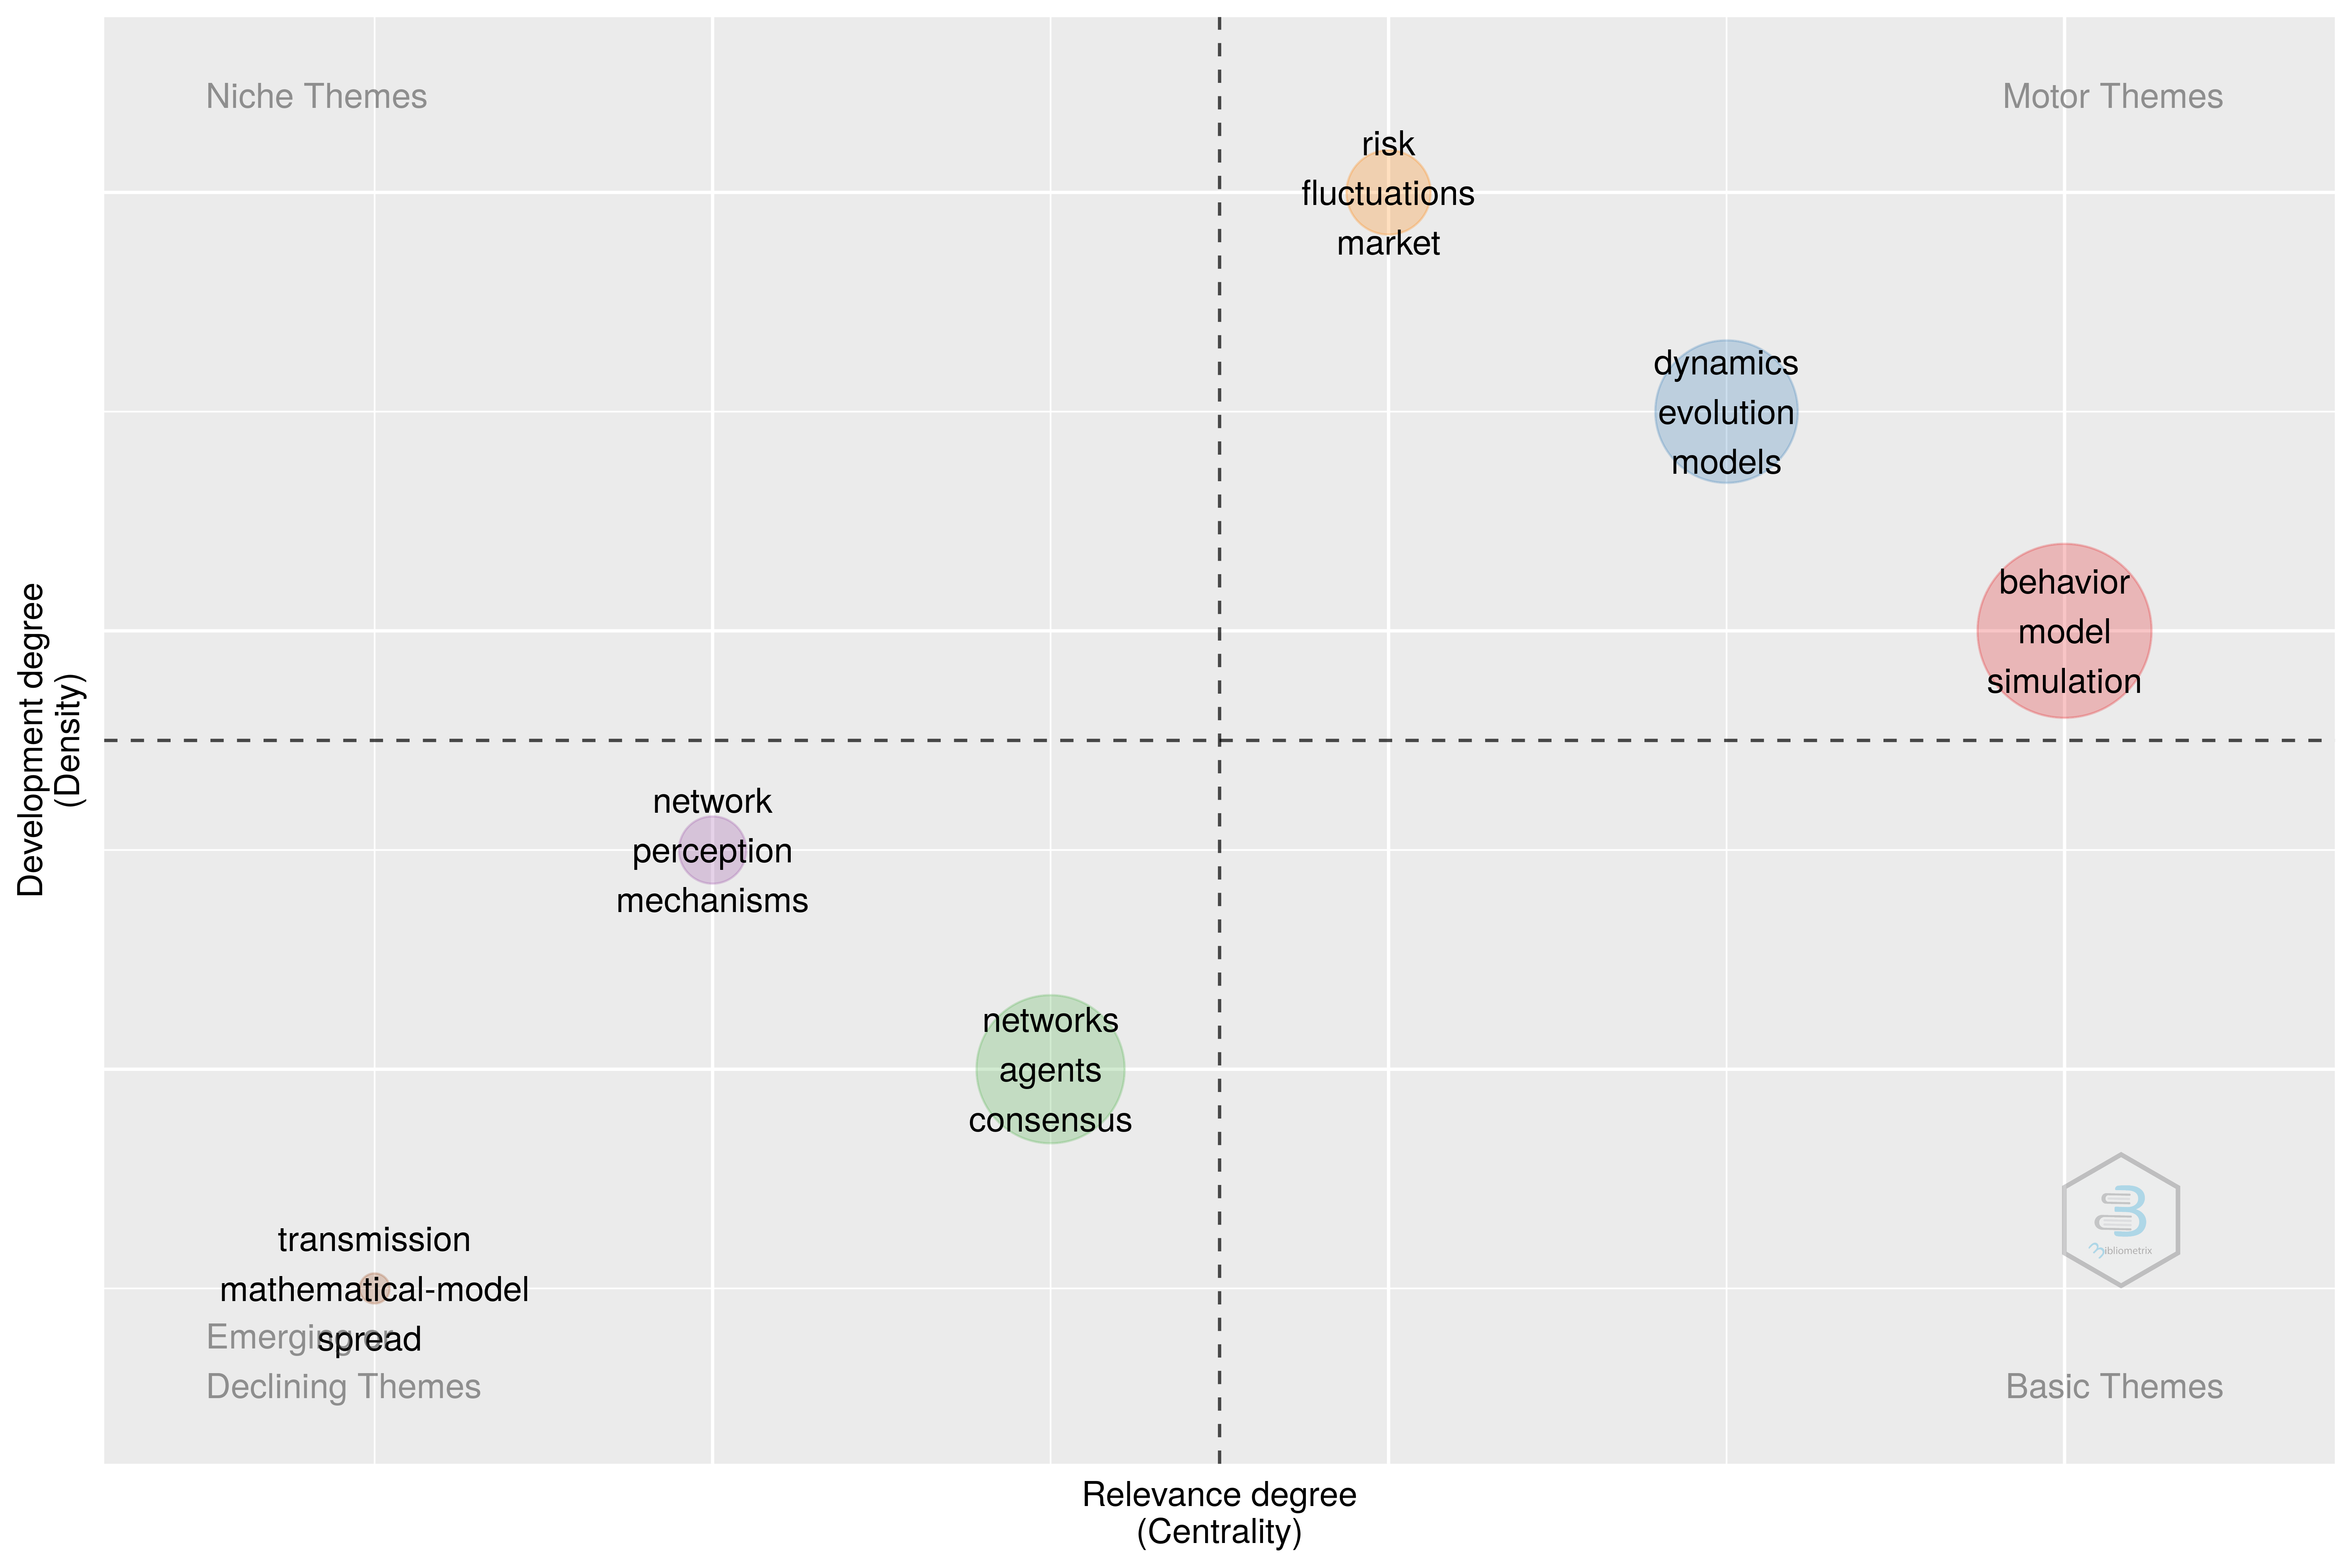
\includegraphics[width=1\textwidth]{experiments/jhcf/PesqBibliogr/SimulacaoMultiagente/WoS-20220203/Estrutura/Conceitual/MASSA2-ThematicMap.png}
    \caption{Mapa temático do  \dataset\ MASSA2@jhcf.}
    \label{fig:MASSA2-ThematicMap}
\end{figure}

\paragraph{Evolução Temática}

\begin{figure}
    \centering
    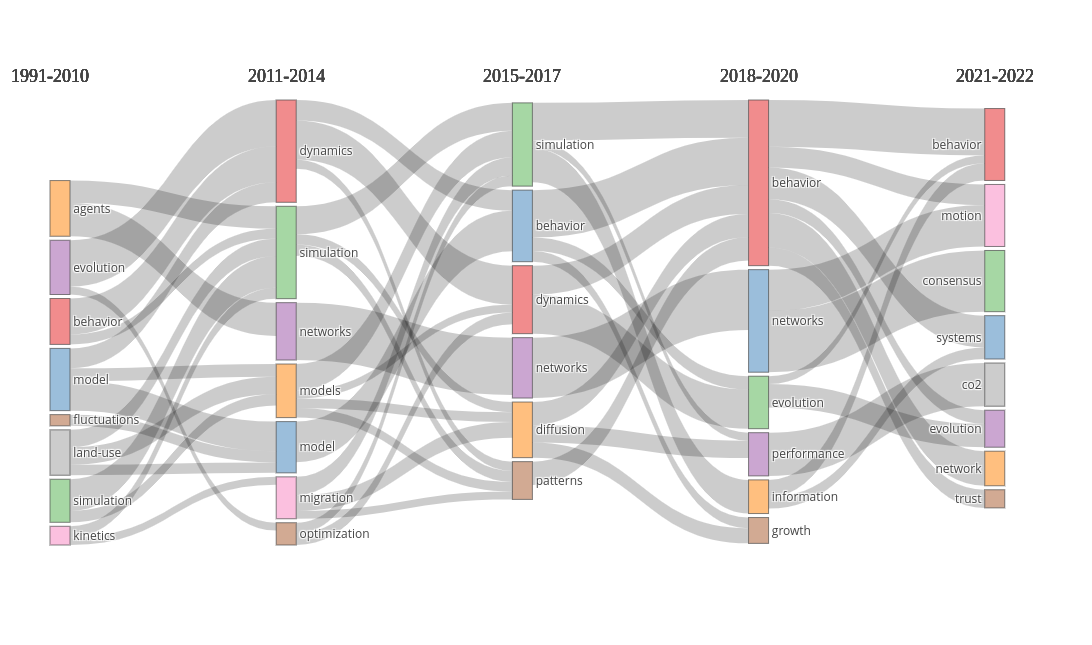
\includegraphics[width=1\textwidth]{experiments/jhcf/PesqBibliogr/SimulacaoMultiagente/WoS-20220203/Estrutura/Conceitual/MASSA2-Thematic-Evolution.png}
    \caption{Evolução temática do  \dataset\ MASSA2@jhcf.}
    \label{fig:MASSA2-ThematicMap}
\end{figure}

\subsubsection{Métricas de redução da dimensionalidade (Análise Fatorial)}

\begin{figure}
    \centering
    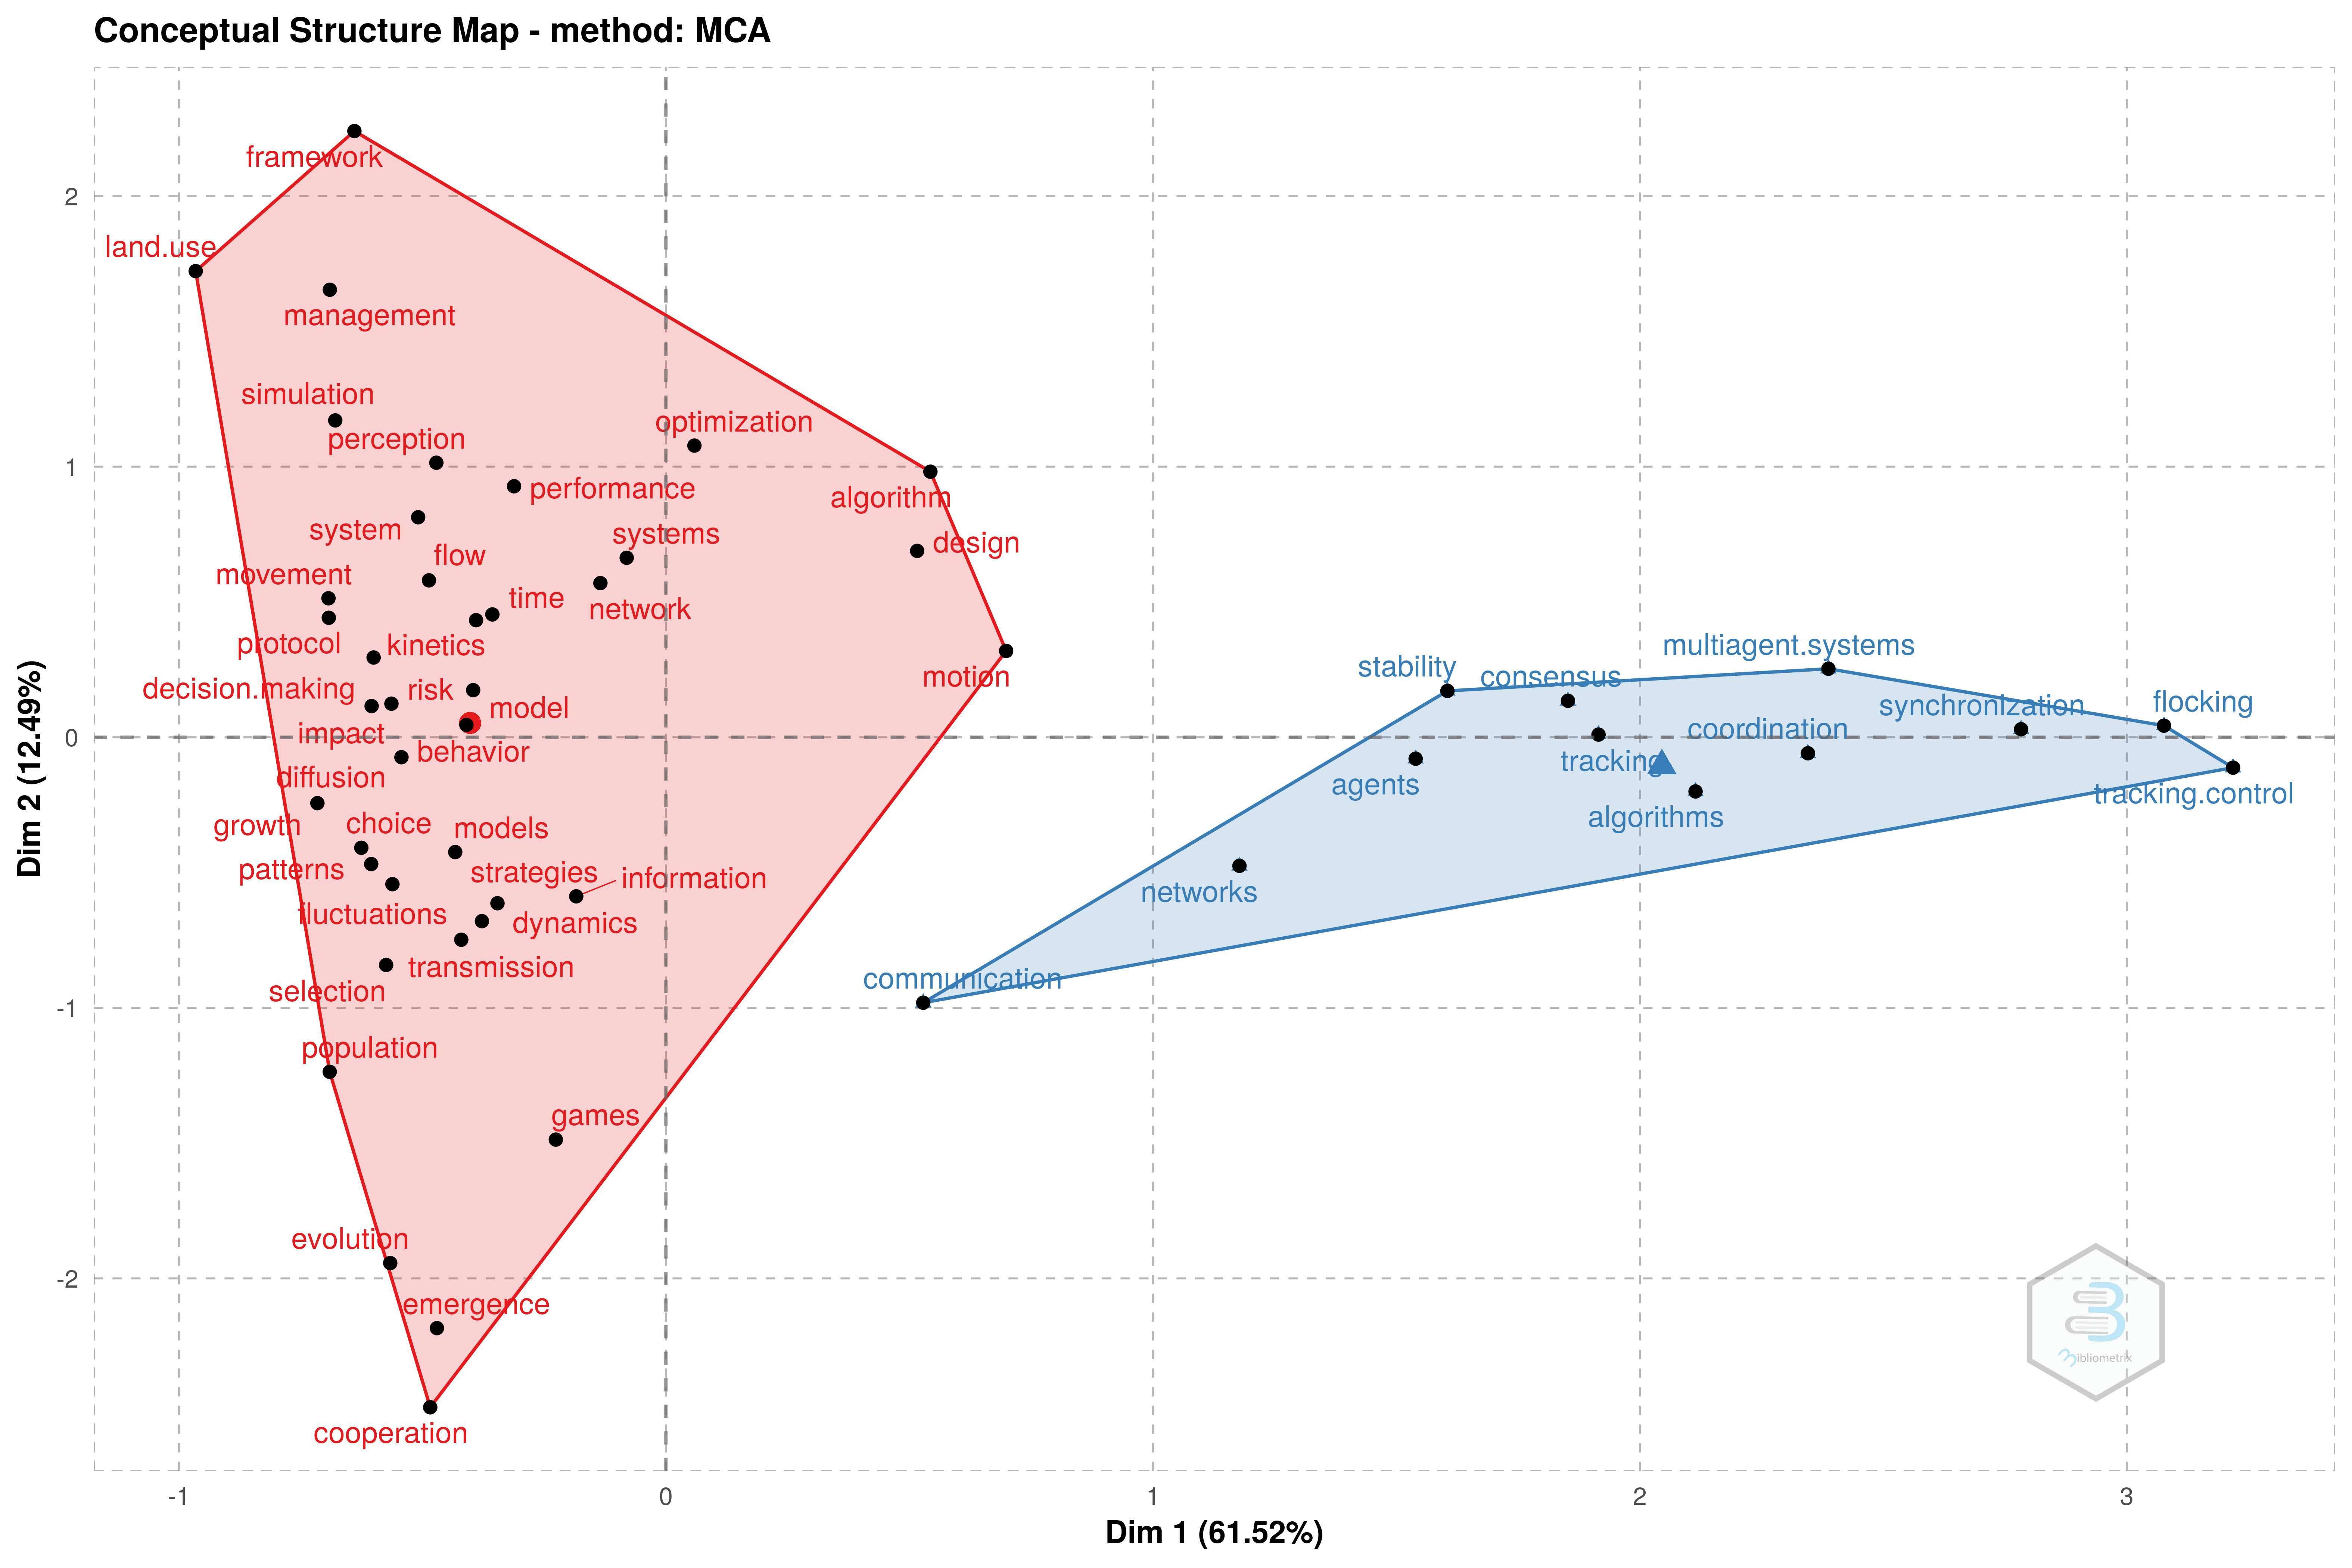
\includegraphics[width=1\textwidth]{experiments/jhcf/PesqBibliogr/SimulacaoMultiagente/WoS-20220203/Estrutura/Conceitual/MASSA2-FactorialAnalysis-MCA-FactorialMap.png}
    \caption{Dimensões de variabilidade mais relevantes, nas palavras-chave do  \dataset\ MASSA2@jhcf.}
    \label{fig:MASSA2-FactorialAnalysis-MCA-FactorialMap}
\end{figure}

\begin{figure}
    \centering
    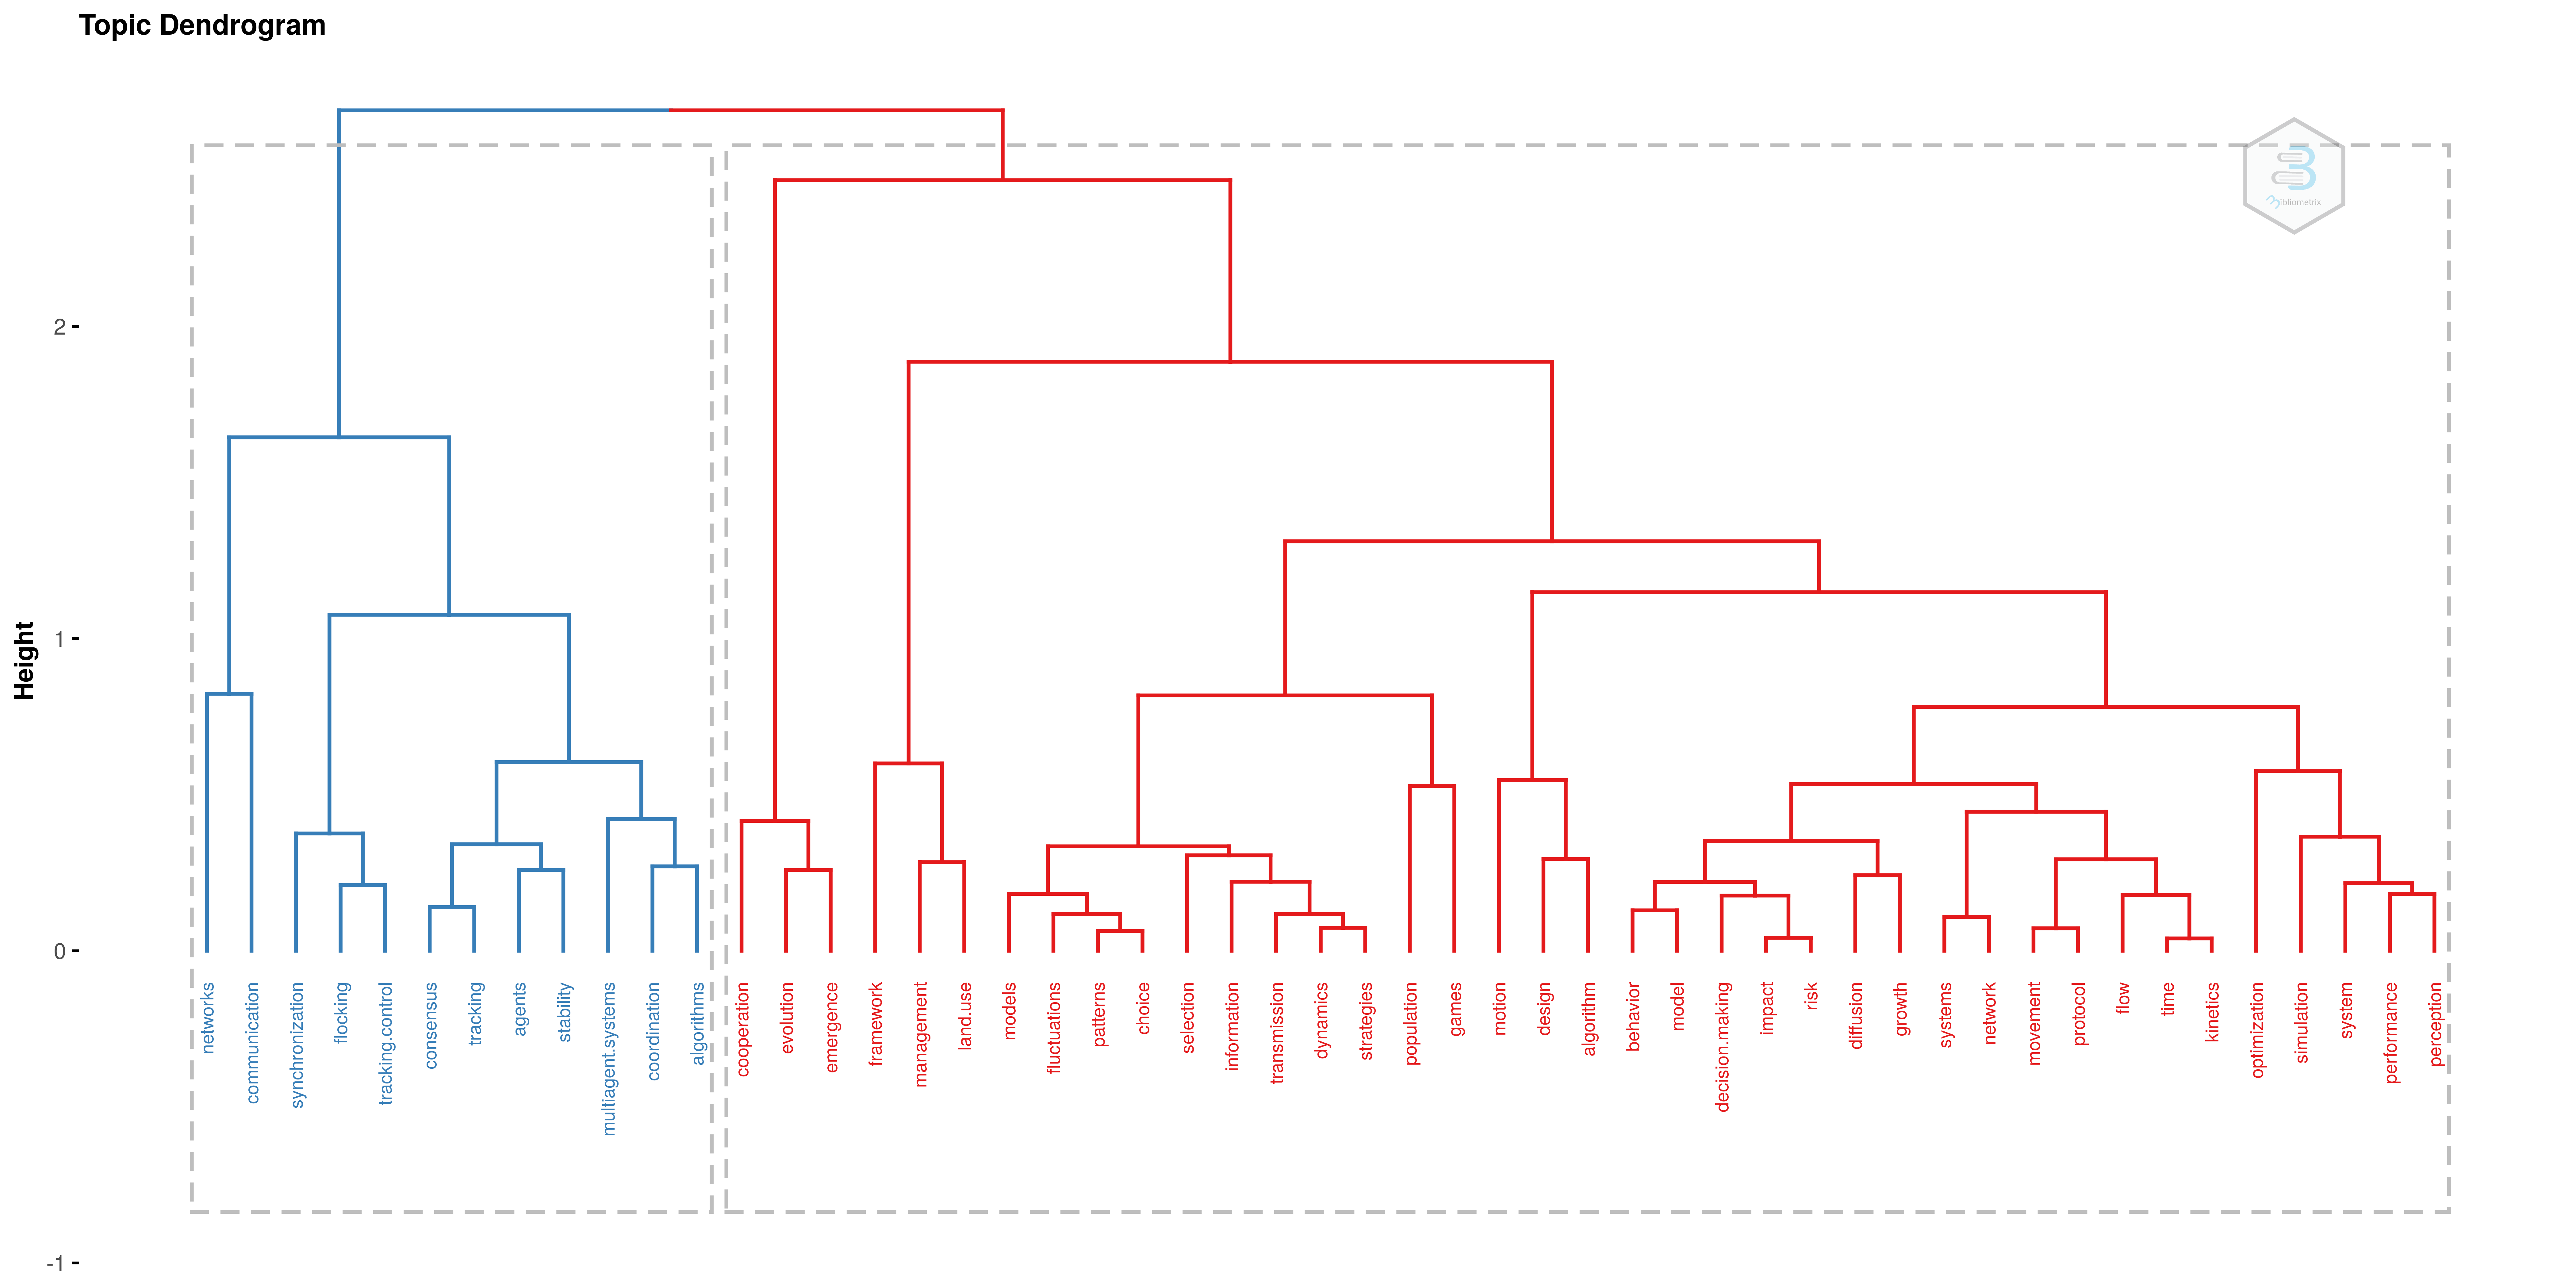
\includegraphics[width=1\textwidth]{experiments/jhcf/PesqBibliogr/SimulacaoMultiagente/WoS-20220203/Estrutura/Conceitual/MASSA2-FactorialAnalysis-MCA-Dendrogram.png}
    \caption{Dendograma das dimensões de variabilidade mais relevantes, nas palavras-chave do  \dataset\ MASSA2@jhcf.}
    \label{fig:MASSA2-FactorialAnalysis-MCA-Dendrogram}
\end{figure}

\begin{figure}
    \centering
    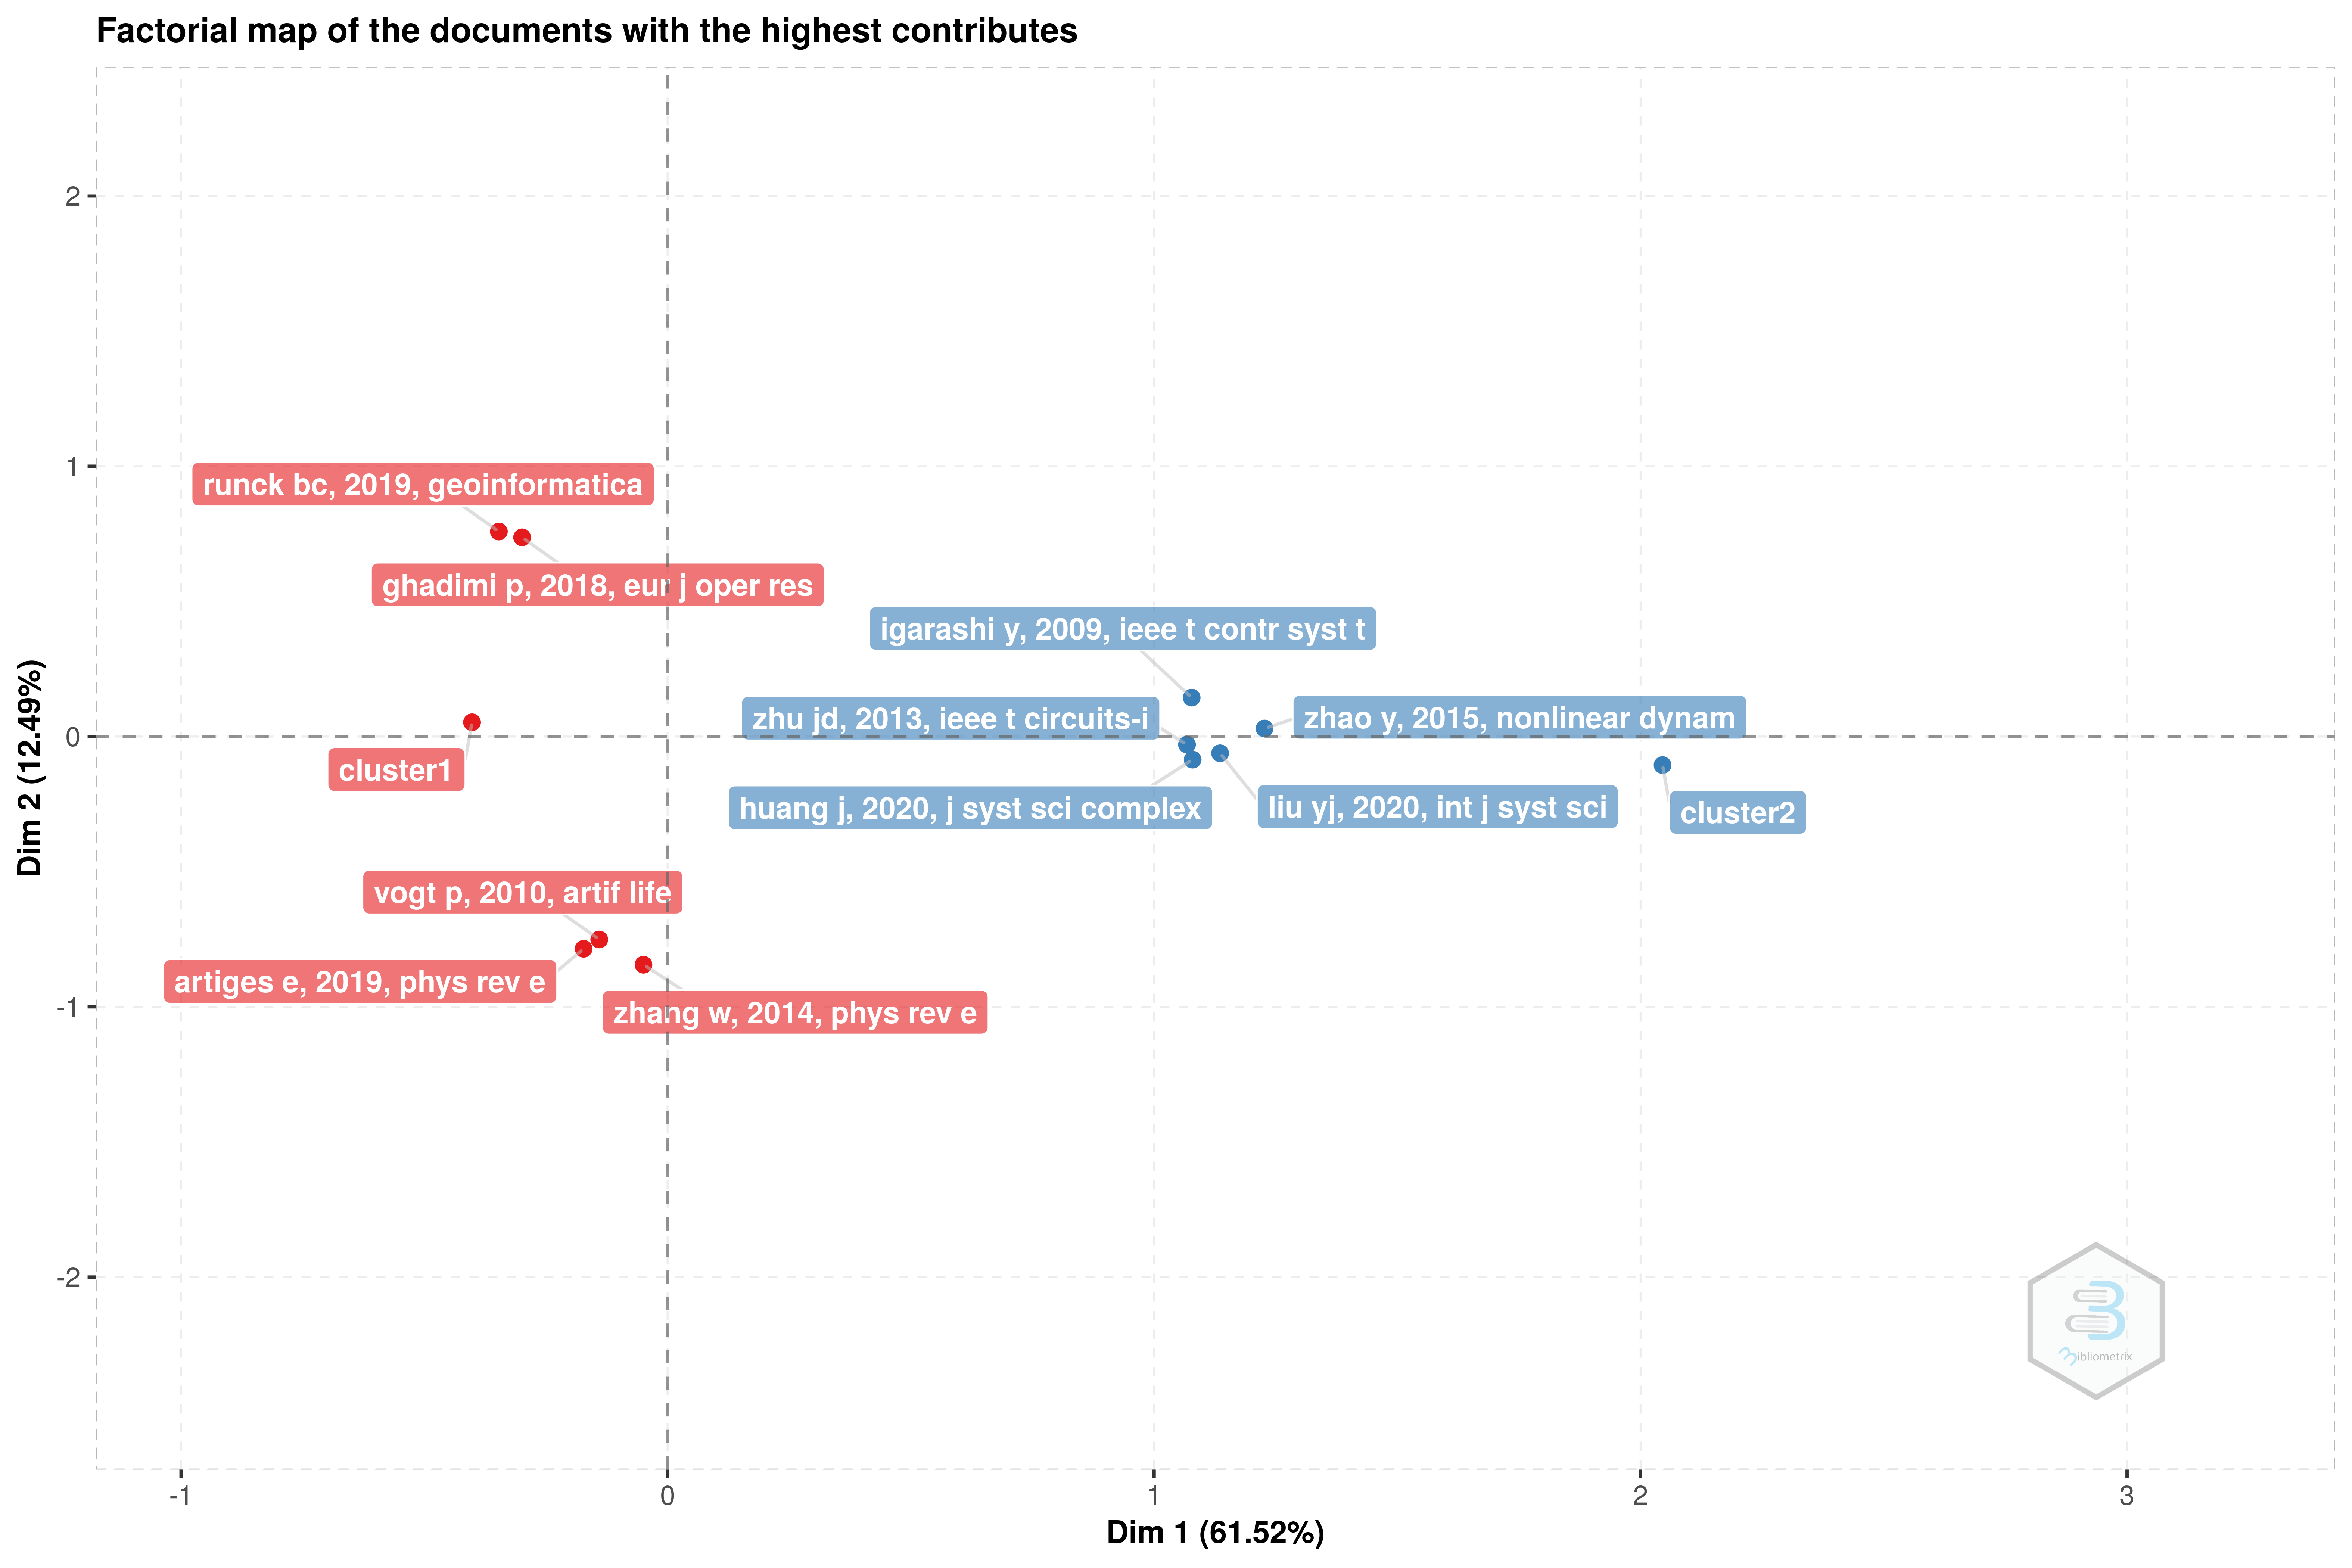
\includegraphics[width=1\textwidth]{experiments/jhcf/PesqBibliogr/SimulacaoMultiagente/WoS-20220203/Estrutura/Conceitual/MASSA2-FactorialAnalysis-MCA-MostContribDocuments.png}
    \caption{Documentos que mais contribuíram para determinar das dimensões de variabilidade mais relevantes, nas palavras-chave do  \dataset\ MASSA2@jhcf.}
    \label{fig:MASSA2-FactorialAnalysis-MCA-MostContribDocuments}
\end{figure}

\subsection{Estrutura Intelectual  do Conhecimento}

Conhecimento científico é produzido por processos intelectuais onde autores de trabalho escolhem deliberadamente referenciar trabalhos de outros, por meio de documentos publicados, que são encaminhados para publicações em fontes de informação de sua escolha, e que evoluem ao longo do tempo.

O Bibliometrix permite exploração da estrutura intelectual do conhecimento, usando basicamente duas abordagens:
\begin{itemize}
    \item Redes de Co-Citação, abordagem bastante comum;
    \item Historiografia, abordagem pouco usual.
\end{itemize}

\subsubsection{Redes de Co-Citação}

\begin{figure}
    \centering
    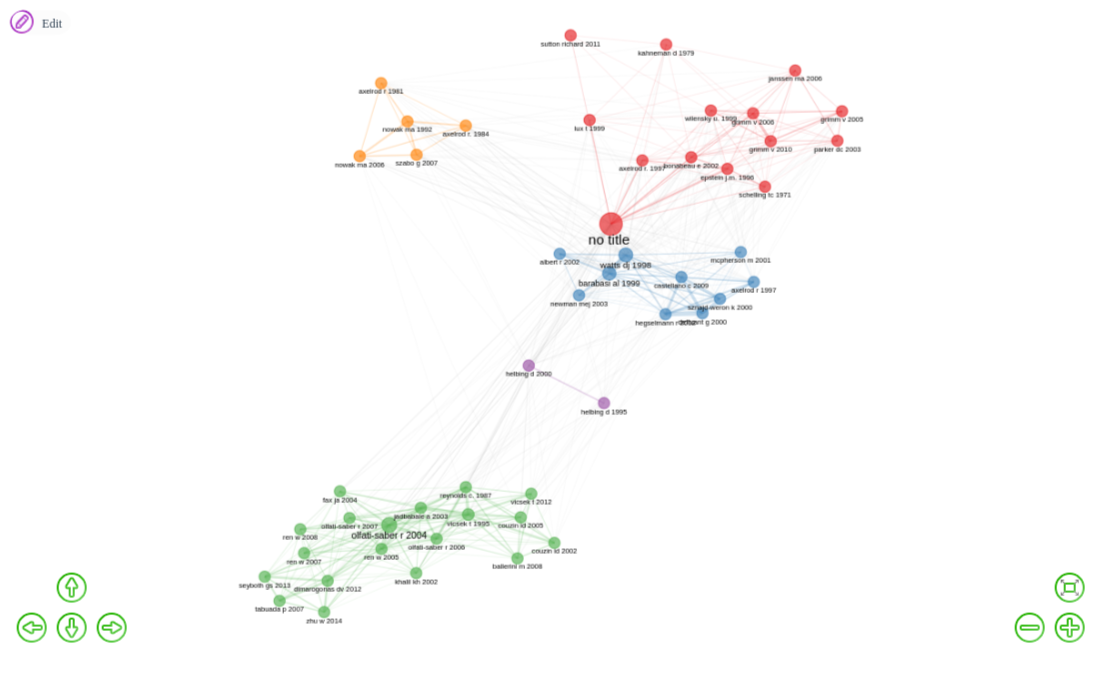
\includegraphics[width=1\textwidth]{experiments/jhcf/PesqBibliogr/SimulacaoMultiagente/WoS-20220203/Estrutura/Intelectual/MASSA2-CoCitation-Network-50-Papers.png}
    \caption{Rede de cocitação entre as 50 referências mais presentes no  \dataset\ MASSA2@jhcf.}
    \label{fig:MASSA2-CoCitation-Network}
\end{figure}

\subsubsection{Historiografia}

\begin{figure}
    \centering
    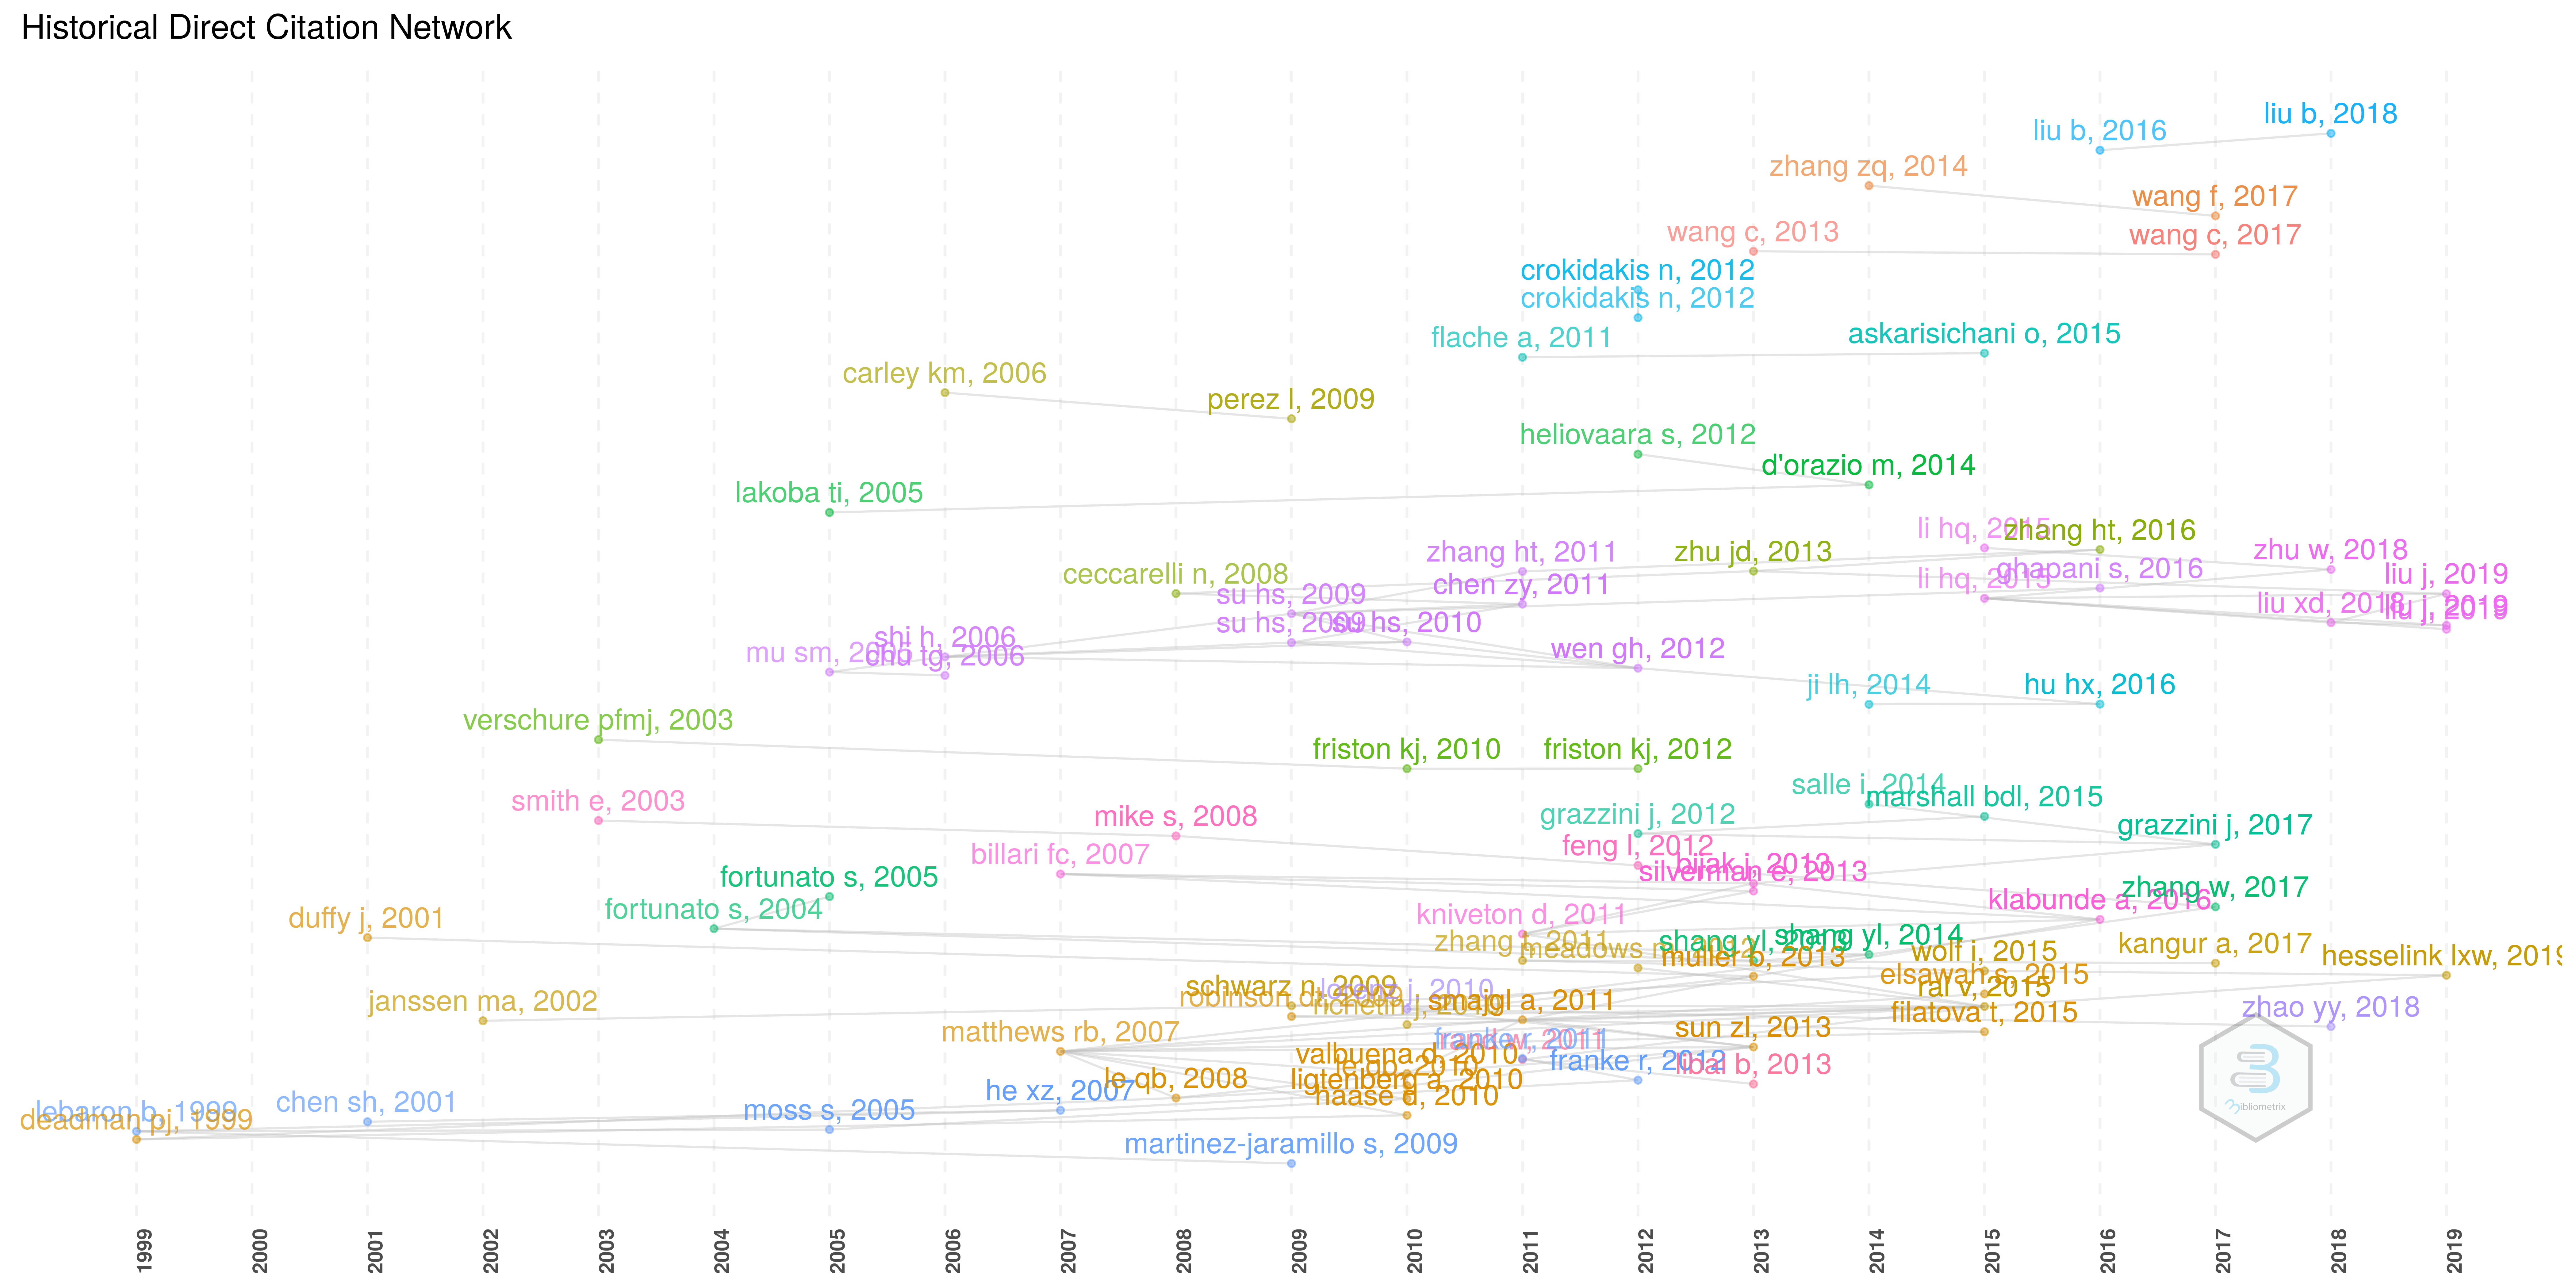
\includegraphics[width=1\textwidth]{experiments/jhcf/PesqBibliogr/SimulacaoMultiagente/WoS-20220203/Estrutura/Intelectual/MASSA2-HistoricalDirectCitationNetwork-100docs.png}
    \caption{Mapa histórico das citações diretas entre os documentos mais evidentes no  \dataset\ MASSA2@jhcf.}
    \label{fig:MASSA2-HistoricalDirectCitationNetwork-100docs}
\end{figure}

\subsection{Estrutura Social  do Conhecimento}

Conhecimento científico é produzido socialmente, por meio de autores trabalhando em conjunto, e uma estrutura de filiações a organizações permanentes ou periódicas, que realizam ou promovem pesquisas, nelas incluídos os centros de pesquisa, universidades, departamentos, institutos, faculdades, eventos, revistas, conferências, e que evoluem ao longo do tempo. A análise da estrutura social do conhecimento evidencia esses relacionamentos, que iniciam no plano pessoal, e evoluem para outros escopos.

\subsubsection{Rede de Colaboração}

\begin{figure}
    \centering
    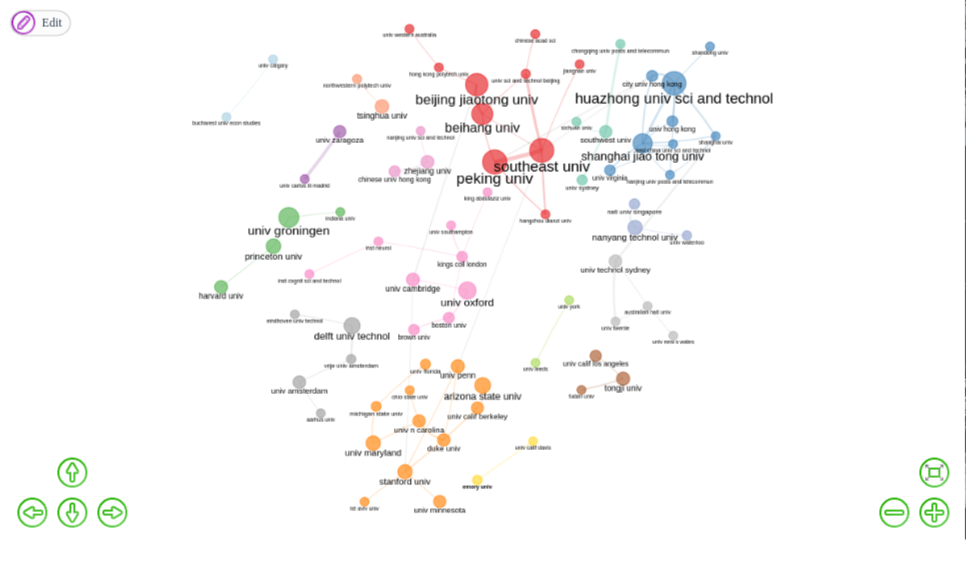
\includegraphics[width=1\textwidth]{experiments/jhcf/PesqBibliogr/SimulacaoMultiagente/WoS-20220203/Estrutura/Social/MASSA2-Collaboration-Network-150instit.png}
    \caption{Rede de colaboração entre as 150 instituições mais evidentes, no  \dataset\ MASSA2@jhcf.}
    \label{fig:MASSA2-Collaboration-Network-150instit}
\end{figure}

\begin{figure}
    \centering
    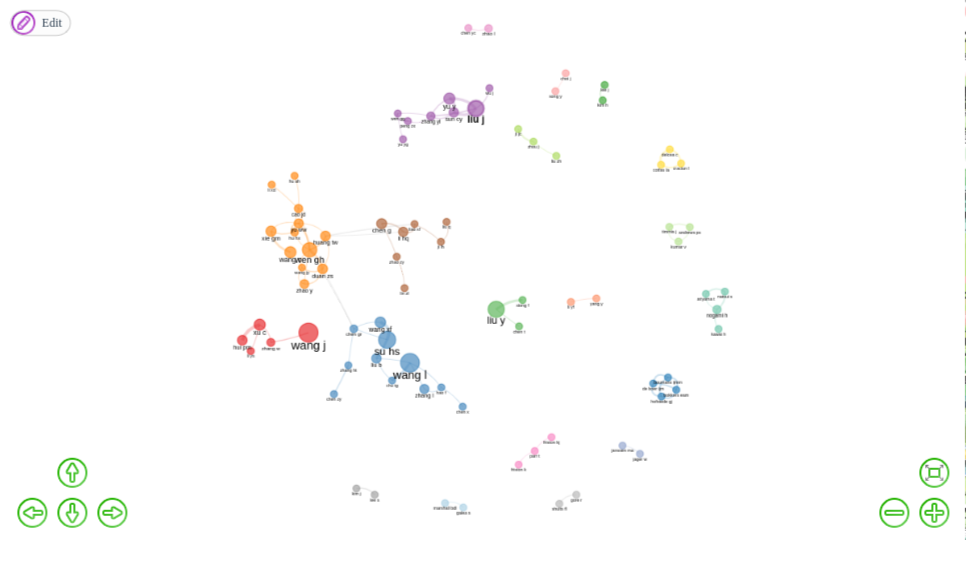
\includegraphics[width=1\textwidth]{experiments/jhcf/PesqBibliogr/SimulacaoMultiagente/WoS-20220203/Estrutura/Social/MASSA2-Collaboration-Network-150authors.png}
    \caption{Rede de colaboração entre os 150 autores mais evidentes, no  \dataset\ MASSA2@jhcf.}
    \label{fig:MASSA2-Collaboration-Network-150authors}
\end{figure}

\begin{figure}
    \centering
    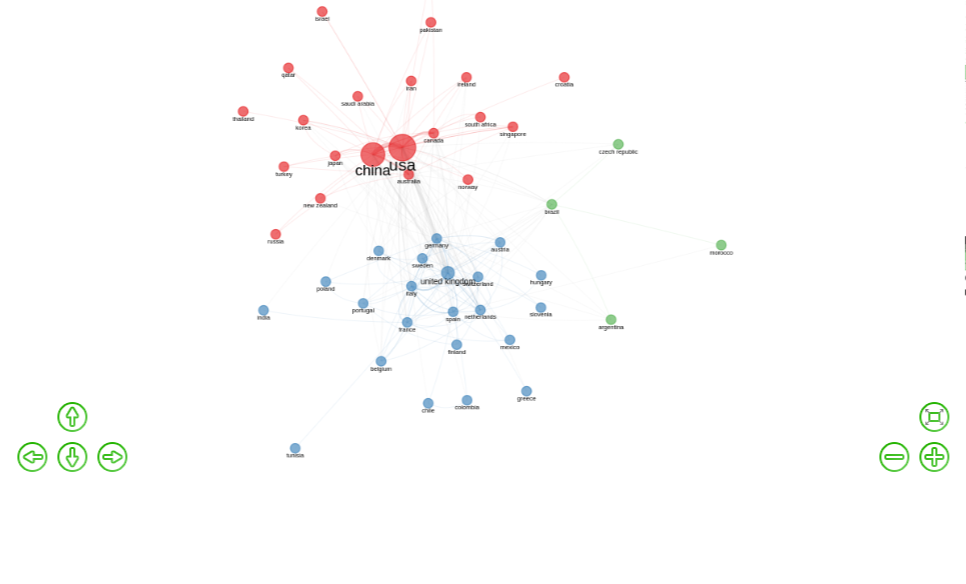
\includegraphics[width=1\textwidth]{experiments/jhcf/PesqBibliogr/SimulacaoMultiagente/WoS-20220203/Estrutura/Social/MASSA2-Collaboration-Network-50country.png}
    \caption{Rede de colaboração entre os 150 países, no  \dataset\ MASSA2@jhcf.}
    \label{fig:MASSA2-Collaboration-Network-50country}
\end{figure}

%\subsubsection{Mapa da Colaboração Mundial}

\section{Análises\label{MASSA2:Analises}}

A pesquisa mundial no tema da simulação multiagente de fenômenos sociais é pontuada por dois grandes temas, ilustrados de forma bastante clara no mapa de estrutura conceitual da figura \ref{fig:MASSA2-FactorialAnalysis-MCA-FactorialMap}, na página \pageref{fig:MASSA2-FactorialAnalysis-MCA-FactorialMap}:
\begin{itemize}
    \item 
(Em azul no mapa) um grupo de pesquisadores que estuda questões ligadas a sistemas de controle, em busca de compreender fenômenos de sincronização, consenso, rastreabilidade, coordenação, rastreamento de agentes artificiais, voando ou navegando em bando e se comunicando em redes com topologia variável. Parecem estar em busca de uma inteligência artificial distribuída e robotizada;
\item (em vermelho no mapa) um grupo mais difuso de pesquisadores, que busca compreender a emergência de fenômenos de natureza bem mais variada, inclusive os que ocorrem em grupos sociais humanos. Esses fenômenos pode ser de cooperação, evolução, participação em jogos, crescimento, difusão de inovações, escolhas, tomadas de decisão, percepção, gerenciamento e uso da terra (no sentido geográfico), formação de preços de ativos financeiros etc. Parecem estar em busca das aplicações das leis gerais dos sistemas complexos adaptativos, bem como na investigação de novos fenômenos que expliquem a dinâmica das sociedades humanas e biológicas.
\end{itemize}

\section{Conclusões}

Este trabalho está incompleto, mas apresenta o arcabouço geral de informações que possibilitam responder às  questões formuladas no início da pesquisa, em \ref{MASSA@jhcf:questoes}, para a qual serão apresentadas breves respostas preliminares:

\subsection{Base de conhecimentos}

Qual a base de conhecimentos científicos produzida em torno do tema simulação multiagente voltada à compreensão de fenômenos sociais, com ênfase em métodos experimentais?
 
Resposta: Ver, em \ref{MASSA2:Analises}, que ela se estrutura em dois grupos principais: um voltado para a inteligência artificial distribuída, baseada em agentes artificiais, como drones, possivelmente com aplicações no campo militar.
O outro grupo é mais abrangente, voltado para a compreensão de fenômenos na sociedade humana, e fundamentado
nos fenômenos emergentes.
Tomando-se também por base os mapas \ref{fig:MASSA2-Co-occurrence-Network-50nodes-louvainclustering.png} e seus detalhamentos em \ref{fig:MASSA2-Cluster1-Co-occurrence-Network-50nodes-louvainclustering.png}, \ref{fig:MASSA2-Cluster2-Co-occurrence-Network-50nodes-louvainclustering.png.png}, percebe-se que esse ultimo grupo pode ser subdidivido em dois: um de ordem mais teórica, representado pelo cluster em \ref{fig:MASSA2-Cluster3-Co-occurrence-Network-50nodes-louvainclustering.png.png}, fundamentado na evolução, possivelmente compreendida como um fenômeno emergente, e um mais aplicado, pesadamente lastreado em simulação, construção de modelos para várias áreas de aplicação.

Nota-se, com base na análise da espectroscopia mais recente das referências bibliográficas do \dataset, sumarizada em \ref{fig:MASSA2-ReferenceSpectroscopy:1971:2019} entre os anos de 1971 e 2019, que a área parece atingir sua maturidade por volta do ano de 2011.

\subsection{Fenômenos sociais}
   
Como a simulação multiagente tem sido usada para compreender fenômenos sociais, com ênfase em métodos experimentais? 

Resposta: Ver \ref{MASSA2:Analises}.

\subsection{Termos e conceitos centrais}

Quais os principais termos e conceitos ligados à frente de pesquisa no tema simulação multiagente de fenômenos sociais, com ênfase em métodos experimentais? 

Resposta: Ver e explorar os mapas das figuras \ref{fig:MASSA2-Co-occurrence-Network-50nodes-louvainclustering.png}, \ref{fig:MASSA2-ThematicMap}, entre outros.

\subsection{Estrutura Social da Comunidade}

Qual a estrutura social da comunidade, se é que existe, que pesquisa sobre o tema simulação multiagente de fenômenos sociais, com ênfase em métodos experimentais?

Resposta: Ver e analisar os mapas das figuras \ref{fig:MASSA2-Collaboration-Network-150authors}, \ref{fig:MASSA2-Collaboration-Network-150instit} e \ref{fig:MASSA2-Collaboration-Network-50country}.

A rede de cocitação 